% Options for packages loaded elsewhere
\PassOptionsToPackage{unicode}{hyperref}
\PassOptionsToPackage{hyphens}{url}
\PassOptionsToPackage{dvipsnames,svgnames,x11names}{xcolor}
%
\documentclass[
  letterpaper,
  DIV=11,
  numbers=noendperiod]{scrreprt}

\usepackage{amsmath,amssymb}
\usepackage{iftex}
\ifPDFTeX
  \usepackage[T1]{fontenc}
  \usepackage[utf8]{inputenc}
  \usepackage{textcomp} % provide euro and other symbols
\else % if luatex or xetex
  \usepackage{unicode-math}
  \defaultfontfeatures{Scale=MatchLowercase}
  \defaultfontfeatures[\rmfamily]{Ligatures=TeX,Scale=1}
\fi
\usepackage{lmodern}
\ifPDFTeX\else  
    % xetex/luatex font selection
\fi
% Use upquote if available, for straight quotes in verbatim environments
\IfFileExists{upquote.sty}{\usepackage{upquote}}{}
\IfFileExists{microtype.sty}{% use microtype if available
  \usepackage[]{microtype}
  \UseMicrotypeSet[protrusion]{basicmath} % disable protrusion for tt fonts
}{}
\makeatletter
\@ifundefined{KOMAClassName}{% if non-KOMA class
  \IfFileExists{parskip.sty}{%
    \usepackage{parskip}
  }{% else
    \setlength{\parindent}{0pt}
    \setlength{\parskip}{6pt plus 2pt minus 1pt}}
}{% if KOMA class
  \KOMAoptions{parskip=half}}
\makeatother
\usepackage{xcolor}
\setlength{\emergencystretch}{3em} % prevent overfull lines
\setcounter{secnumdepth}{5}
% Make \paragraph and \subparagraph free-standing
\ifx\paragraph\undefined\else
  \let\oldparagraph\paragraph
  \renewcommand{\paragraph}[1]{\oldparagraph{#1}\mbox{}}
\fi
\ifx\subparagraph\undefined\else
  \let\oldsubparagraph\subparagraph
  \renewcommand{\subparagraph}[1]{\oldsubparagraph{#1}\mbox{}}
\fi

\usepackage{color}
\usepackage{fancyvrb}
\newcommand{\VerbBar}{|}
\newcommand{\VERB}{\Verb[commandchars=\\\{\}]}
\DefineVerbatimEnvironment{Highlighting}{Verbatim}{commandchars=\\\{\}}
% Add ',fontsize=\small' for more characters per line
\usepackage{framed}
\definecolor{shadecolor}{RGB}{241,243,245}
\newenvironment{Shaded}{\begin{snugshade}}{\end{snugshade}}
\newcommand{\AlertTok}[1]{\textcolor[rgb]{0.68,0.00,0.00}{#1}}
\newcommand{\AnnotationTok}[1]{\textcolor[rgb]{0.37,0.37,0.37}{#1}}
\newcommand{\AttributeTok}[1]{\textcolor[rgb]{0.40,0.45,0.13}{#1}}
\newcommand{\BaseNTok}[1]{\textcolor[rgb]{0.68,0.00,0.00}{#1}}
\newcommand{\BuiltInTok}[1]{\textcolor[rgb]{0.00,0.23,0.31}{#1}}
\newcommand{\CharTok}[1]{\textcolor[rgb]{0.13,0.47,0.30}{#1}}
\newcommand{\CommentTok}[1]{\textcolor[rgb]{0.37,0.37,0.37}{#1}}
\newcommand{\CommentVarTok}[1]{\textcolor[rgb]{0.37,0.37,0.37}{\textit{#1}}}
\newcommand{\ConstantTok}[1]{\textcolor[rgb]{0.56,0.35,0.01}{#1}}
\newcommand{\ControlFlowTok}[1]{\textcolor[rgb]{0.00,0.23,0.31}{#1}}
\newcommand{\DataTypeTok}[1]{\textcolor[rgb]{0.68,0.00,0.00}{#1}}
\newcommand{\DecValTok}[1]{\textcolor[rgb]{0.68,0.00,0.00}{#1}}
\newcommand{\DocumentationTok}[1]{\textcolor[rgb]{0.37,0.37,0.37}{\textit{#1}}}
\newcommand{\ErrorTok}[1]{\textcolor[rgb]{0.68,0.00,0.00}{#1}}
\newcommand{\ExtensionTok}[1]{\textcolor[rgb]{0.00,0.23,0.31}{#1}}
\newcommand{\FloatTok}[1]{\textcolor[rgb]{0.68,0.00,0.00}{#1}}
\newcommand{\FunctionTok}[1]{\textcolor[rgb]{0.28,0.35,0.67}{#1}}
\newcommand{\ImportTok}[1]{\textcolor[rgb]{0.00,0.46,0.62}{#1}}
\newcommand{\InformationTok}[1]{\textcolor[rgb]{0.37,0.37,0.37}{#1}}
\newcommand{\KeywordTok}[1]{\textcolor[rgb]{0.00,0.23,0.31}{#1}}
\newcommand{\NormalTok}[1]{\textcolor[rgb]{0.00,0.23,0.31}{#1}}
\newcommand{\OperatorTok}[1]{\textcolor[rgb]{0.37,0.37,0.37}{#1}}
\newcommand{\OtherTok}[1]{\textcolor[rgb]{0.00,0.23,0.31}{#1}}
\newcommand{\PreprocessorTok}[1]{\textcolor[rgb]{0.68,0.00,0.00}{#1}}
\newcommand{\RegionMarkerTok}[1]{\textcolor[rgb]{0.00,0.23,0.31}{#1}}
\newcommand{\SpecialCharTok}[1]{\textcolor[rgb]{0.37,0.37,0.37}{#1}}
\newcommand{\SpecialStringTok}[1]{\textcolor[rgb]{0.13,0.47,0.30}{#1}}
\newcommand{\StringTok}[1]{\textcolor[rgb]{0.13,0.47,0.30}{#1}}
\newcommand{\VariableTok}[1]{\textcolor[rgb]{0.07,0.07,0.07}{#1}}
\newcommand{\VerbatimStringTok}[1]{\textcolor[rgb]{0.13,0.47,0.30}{#1}}
\newcommand{\WarningTok}[1]{\textcolor[rgb]{0.37,0.37,0.37}{\textit{#1}}}

\providecommand{\tightlist}{%
  \setlength{\itemsep}{0pt}\setlength{\parskip}{0pt}}\usepackage{longtable,booktabs,array}
\usepackage{calc} % for calculating minipage widths
% Correct order of tables after \paragraph or \subparagraph
\usepackage{etoolbox}
\makeatletter
\patchcmd\longtable{\par}{\if@noskipsec\mbox{}\fi\par}{}{}
\makeatother
% Allow footnotes in longtable head/foot
\IfFileExists{footnotehyper.sty}{\usepackage{footnotehyper}}{\usepackage{footnote}}
\makesavenoteenv{longtable}
\usepackage{graphicx}
\makeatletter
\def\maxwidth{\ifdim\Gin@nat@width>\linewidth\linewidth\else\Gin@nat@width\fi}
\def\maxheight{\ifdim\Gin@nat@height>\textheight\textheight\else\Gin@nat@height\fi}
\makeatother
% Scale images if necessary, so that they will not overflow the page
% margins by default, and it is still possible to overwrite the defaults
% using explicit options in \includegraphics[width, height, ...]{}
\setkeys{Gin}{width=\maxwidth,height=\maxheight,keepaspectratio}
% Set default figure placement to htbp
\makeatletter
\def\fps@figure{htbp}
\makeatother
\newlength{\cslhangindent}
\setlength{\cslhangindent}{1.5em}
\newlength{\csllabelwidth}
\setlength{\csllabelwidth}{3em}
\newlength{\cslentryspacingunit} % times entry-spacing
\setlength{\cslentryspacingunit}{\parskip}
\newenvironment{CSLReferences}[2] % #1 hanging-ident, #2 entry spacing
 {% don't indent paragraphs
  \setlength{\parindent}{0pt}
  % turn on hanging indent if param 1 is 1
  \ifodd #1
  \let\oldpar\par
  \def\par{\hangindent=\cslhangindent\oldpar}
  \fi
  % set entry spacing
  \setlength{\parskip}{#2\cslentryspacingunit}
 }%
 {}
\usepackage{calc}
\newcommand{\CSLBlock}[1]{#1\hfill\break}
\newcommand{\CSLLeftMargin}[1]{\parbox[t]{\csllabelwidth}{#1}}
\newcommand{\CSLRightInline}[1]{\parbox[t]{\linewidth - \csllabelwidth}{#1}\break}
\newcommand{\CSLIndent}[1]{\hspace{\cslhangindent}#1}

\KOMAoption{captions}{tableheading}
\makeatletter
\makeatother
\makeatletter
\@ifpackageloaded{bookmark}{}{\usepackage{bookmark}}
\makeatother
\makeatletter
\@ifpackageloaded{caption}{}{\usepackage{caption}}
\AtBeginDocument{%
\ifdefined\contentsname
  \renewcommand*\contentsname{Table of contents}
\else
  \newcommand\contentsname{Table of contents}
\fi
\ifdefined\listfigurename
  \renewcommand*\listfigurename{List of Figures}
\else
  \newcommand\listfigurename{List of Figures}
\fi
\ifdefined\listtablename
  \renewcommand*\listtablename{List of Tables}
\else
  \newcommand\listtablename{List of Tables}
\fi
\ifdefined\figurename
  \renewcommand*\figurename{Figure}
\else
  \newcommand\figurename{Figure}
\fi
\ifdefined\tablename
  \renewcommand*\tablename{Table}
\else
  \newcommand\tablename{Table}
\fi
}
\@ifpackageloaded{float}{}{\usepackage{float}}
\floatstyle{ruled}
\@ifundefined{c@chapter}{\newfloat{codelisting}{h}{lop}}{\newfloat{codelisting}{h}{lop}[chapter]}
\floatname{codelisting}{Listing}
\newcommand*\listoflistings{\listof{codelisting}{List of Listings}}
\usepackage{amsthm}
\theoremstyle{definition}
\newtheorem{exercise}{Exercise}[chapter]
\theoremstyle{definition}
\newtheorem{example}{Example}[chapter]
\theoremstyle{remark}
\AtBeginDocument{\renewcommand*{\proofname}{Proof}}
\newtheorem*{remark}{Remark}
\newtheorem*{solution}{Solution}
\makeatother
\makeatletter
\@ifpackageloaded{caption}{}{\usepackage{caption}}
\@ifpackageloaded{subcaption}{}{\usepackage{subcaption}}
\makeatother
\makeatletter
\@ifpackageloaded{tcolorbox}{}{\usepackage[skins,breakable]{tcolorbox}}
\makeatother
\makeatletter
\@ifundefined{shadecolor}{\definecolor{shadecolor}{rgb}{.97, .97, .97}}
\makeatother
\makeatletter
\makeatother
\makeatletter
\makeatother
\ifLuaTeX
  \usepackage{selnolig}  % disable illegal ligatures
\fi
\IfFileExists{bookmark.sty}{\usepackage{bookmark}}{\usepackage{hyperref}}
\IfFileExists{xurl.sty}{\usepackage{xurl}}{} % add URL line breaks if available
\urlstyle{same} % disable monospaced font for URLs
\hypersetup{
  pdftitle={Introduction to Computational Finance and Financial Econometrics with R},
  pdfauthor={Eric Zivot},
  colorlinks=true,
  linkcolor={blue},
  filecolor={Maroon},
  citecolor={Blue},
  urlcolor={Blue},
  pdfcreator={LaTeX via pandoc}}

\title{Introduction to Computational Finance and Financial Econometrics
with R}
\author{Eric Zivot}
\date{2026-08-31}

\begin{document}
\maketitle
\ifdefined\Shaded\renewenvironment{Shaded}{\begin{tcolorbox}[breakable, boxrule=0pt, enhanced, interior hidden, borderline west={3pt}{0pt}{shadecolor}, frame hidden, sharp corners]}{\end{tcolorbox}}\fi

\renewcommand*\contentsname{Table of contents}
{
\hypersetup{linkcolor=}
\setcounter{tocdepth}{2}
\tableofcontents
}
\bookmarksetup{startatroot}

\hypertarget{preface}{%
\chapter*{Preface}\label{preface}}
\addcontentsline{toc}{chapter}{Preface}

\markboth{Preface}{Preface}

I am a Professor of Economics at the University of Washington (UW) where
I teach the class \emph{Introductional to Computational Finance and
Financial Econometrics} (ECON 424). This course started as an
experiment. In the winter quarter of 1998 I was on leave visiting the
economics department at the University of California Los Angeles (UCLA).
To help pay for my leave I, I arranged to teach a standard undergraduate
econometrics course. My research at the time was moving toward financial
econometrics and I thought it would be fun to teach an econometrics
course with most of the examples motivated by financial applications. I
thought that combining econometrics and statistics topics with financial
applications would be a very effective and popular way of getting
students interested in learning and applying econometrics. My intuition
was right. My students at UCLA loved the version of the course I
offered. After returning to the University of Washington, I created the
upper division undergraduate course \emph{Introduction to Computational
and Financial Econometrics}. The course was an immediate hit. This book
evolved from my lecture notes for the course.

\emph{Who is the book written for? What background is required?}

My ECON 424 course is taken mainly by senior economics majors who are
pursuing the more quantitative Bachelor of Science Degree in Economics
at UW. These students typically have at least one year of calculus,
intermediate microeconomics with some calculus (so they are exposed to
optimization under constraints using Lagrange multipliers), and an
introductory course in probability and statistics for economics majors.
Some students have taken a course in linear algebra, some have taken an
introductory econometrics course, and some have taken a financial
economics course. I find that the typical introductory probability and
statistics course is at a lower level than is needed for much of the
material in my course. Ideally, students should have an intermediate
probability and statistics course that uses calculus\footnote{Insert
  reference to recent MIT Press book here}. As a result, I spend a week
at the beginning of the course doing a review of random variables and
probability that uses basic calculus. A key part of the review is the
manipulation of random variables, computing expectations of functions of
random variables, etc., so that the students have the necessary tools to
work with simple probabilistic models for asset returns. After the
review of probability theory I introduce some basic time series concepts
(e.g., stochastic processes and stationarity), as these concepts are
often not taught in introductory probability and statistics classes, and
I also do a quick review of basic matrix algebra that I use throughout
the course. The use of matrix algebra is important for two reasons.
First, most introductory textbook treatments of portfolio theory show
calculations for the simple case of two assets and then talk about how
the calculations extend to the general case of many assets but do not
show how this is done. Hence, students are not capable of implementing
the theory for real world portfolios. I emphasize that with knowledge of
just a little bit of matrix algebra - essentially matrix addition,
multiplication, inversion, and some matrix differential calculus - the
general analysis of portfolio theory can be easily learned and
implemented. Second, R is a vectorized and matrix programming language
and so basic knowledge of matrix algebra allows students to easily
understand and implement the R code for portfolio analysis.

\emph{Main topics covered in the book}

After the review material, I jump into descriptive statistical analysis
of historical financial time series data. I emphasize that my approach
to building models for asset returns is based on first looking at the
historical data and studying its properties. I start by telling students
to pretend that observed returns on assets are realizations from some
unknown covariance stationary stochastic process. I review common
graphical and numerical descriptive statistics (e.g., histograms,
QQ-plots, sample mean, variance, correlation, etc.). The goal of
descriptive statistical analysis is to compile a collection of
``stylized facts'' that can be used as building blocks for probabilistic
models for asset returns. For example, I show that monthly asset returns
are typically uncorrelated over time, have empirical distributions
(histograms) that look like normal bell curves, have means close to
zero, are positively correlated with other assets, etc. I also emphasize
that some ``stylized facts'' of asset returns appear to stay the same
for different investment horizons (daily, weekly, and monthly returns
are uncorrelated) and some do not (e.g., daily and weekly returns have
fatter tails than the normal and show evidence of nonlinear time
dependence in higher moments)

\emph{Why us R?}

My early versions of \emph{Introduction to Computational and Financial
Econometrics} used Microsoft Excel as the main software tool as R was
not yet around then. My decision to use Excel was for the students'
benefit. Students having experience with Excel was, and still is, in
high demand by employers in the finance industry. It is often said,
``the financial world runs out of an Excel spreadsheet''. However, Excel
is not a good tool for doing statistics. Even though you \emph{can} do
statistical analysis in Excel, does not mean that you \emph{should} do
statistical analysis in Excel. I searched for Excel add-ins to make
doing statistical analysis in Excel easier but I did not like what was
available. Everything changed when I met Professor Doug Martin from the
UW statistics department. Doug founded the company who created S-PLUS,
the commercial version of the S statistical programming language
developed by John Chambers at Bell Labs (R became the open source
version of S in 2000). S is a beautiful language for exploratory data
and statistical analysis and S-PLUS made it easily available to students
on windows PCs. In the early 2000s I used Excel together with S-PLUS for
my course. This hybrid approach worked well but the difficulties of
getting student licenses at the beginning of the quarter was always a
headache. As R matured in the mid to late 2000s, I made the switch from
S-PLUS to R and never looked back. As the course evolved and R became
more commonly used in the financial world, and Rstudio became the
integrated developer environment of choice for R, I eventually dropped
the use of Excel and focused solely on R for the applications and
examples in the book.

Many economics students lack experience with programming languages and
some find R a difficult language to learn and use. My approach to
dealing with this reality is to provide all of the R code to do
calculations in the class lectures, in the textbook examples, and on
homework assignments. In this way students do not have to worry about
the coding aspect of the class and can more easily concentrate on the
concepts of computational finance and financial econometrics. I find
that students learn to use R quite well this way -- learning by doing --
and most students are quite proficient in R by the end of the course.

There are a lot of free resources on the web for learning R. In my
Coursera course I partnered with DataCamp to provide a web-based
learning environment for R tailored to the course material. I have found
that this has substantially lowered the learning curve for many
students. Student mostly use either a MAC or PC for their work (a few
geeks use UNIX). I found that some things didn't always work well across
platforms (usually issues with the file system). In 2014, I required
students to use Rstudio as the environment for using R. This makes
learning and working with R even easier. Another advantage of using
Rstudio is that my lecture notes and homework assignments are be created
using Rmarkdown.

\emph{Longer print book}

(Shorter ebook). This book is based on my University of Washington
sponsored Coursera course Introduction to Computational Finance and
Financial Econometrics that has been running every quarter on Coursera
since 2013. This Coursera course is based on the Summer 2013 offering of
my University of Washington advanced undergraduate economics course of
the same name. At the time, my UW course was part of a three course
summer certificate in Fundamentals of Quantitative Finance offered by
the Professional Masters Program in Computational Finance \& Risk
Management that was video-recorded and available for online students. An
edited version of this course became the Coursera course. The popularity
of the course encouraged me to convert the class notes for the course
into a short book.

The book was typeset using Lyx with all of the R code examples embedded
into the document and evaluated using knitr. I am extremely grateful to
Yihui Xie for writing his wonderful book Dynamics Documents with R and
knitr as this book would not have been possible without it. I am a firm
believer in the ``reproducible research paradigm''.

The book's accompanying R package \texttt{introcompfinr} contains all of
the financial data used for the examples presented in the book as well
as a number of R functions written by me for estimating some simple
models of asset returns, and doing portfolio and risk analysis. The
package is freely available on GitHub at
https://github.com/ezivot/introcompfinr and can be installed using:

\begin{Shaded}
\begin{Highlighting}[]
\FunctionTok{install.packages}\NormalTok{(}\StringTok{"pak"}\NormalTok{)}
\NormalTok{pak}\SpecialCharTok{::}\FunctionTok{pak}\NormalTok{(}\StringTok{"ezivot/introcompfinr"}\NormalTok{).}
\end{Highlighting}
\end{Shaded}

\emph{How is this book different from other introductory book on
financial econometrics?}

There are now many good books written on the topic of
computational/quantitative finance and financial econometrics with
examples in R at various levels of sophistication. Books written for
advanced U.S. undergraduates include Carmona (2014) and Tsay (2012).
Books written for Masters students in computational finance or financial
engineering courses include Fan and Yao (20xx), Lai and Xing (2008),
Ruppert and Matteson (2015) and Tsay (2010). All of these books assume
the readers have a broader mathematical and statistical background than
what I assume here. Hence, this book is truly an ``introduction'' to the
methods of computational finance and financial econometrics and is
appropriate for undergraduate economics and finance majors at
Universities worldwide. Another feature that distinguishes this book
from others is the extensive use of R and illustrated R code throughout
the book. In this regard, this book is a ``hands on'' book in which the
student can readily execute the R examples on their own computer while
reading the book. This allows the student to also learn R as well as the
concepts in the book.

Eric Zivot\\
Seattle, Washington\\
August 2026

\bookmarksetup{startatroot}

\hypertarget{acknowledgments}{%
\chapter*{Acknowledgments}\label{acknowledgments}}
\addcontentsline{toc}{chapter}{Acknowledgments}

\markboth{Acknowledgments}{Acknowledgments}

Many people have helped with the development of this book. First and
foremost, I would like to thank the students at UW who have taken my
course over the last fifteen years. I have received countless comments,
corrections, and suggestions that have greatly improved the exposition
and material in the book.

A lot of how I think about the statistical analysis of financial data
has been shaped by many discussions and interactions with my long-term
colleague and good friend R. Douglas Martin. Doug introduced me to the S
language and I had the pleasure of working with him at Insightful where
we developed the S+FinMetrics module for S-PLUS and I wrote the book
\emph{Modeling Financial Time Series with S-PLUS} with my former
Ph.D.~student Jiahui (Jeffrey) Wang.

My very patient wife Nina Sidneva carefully proof-read many early
versions of the chapters as they were under development and caught many
of my stupid errors. Xiao Yin proof-read most of the chapters after I
converted my Latex notes to Lyx and incorporated the R examples with
\texttt{knitr}. I could not have written the book without the expert
technical help from Bethany Yollin and the wonderful book \emph{Dynamics
Documents with R and knitr} by Yihui Xie. Bethany helped with the
conversion of my Latex notes to Lyx and the incorporation of the R
examples in the text using \texttt{knitr}. She also helped to develop
and maintain an early version the book's R package,
\texttt{IntroCompfinR}. Any problem I found with Lyx and \texttt{knitr}
was solved by referring to Yihui's book. In 2020 I decided to migrate
the book from Lyx to Rmarkdown so that everything could be managed
within Rstudio and the book could be generated using \texttt{bookdown}.
My UW PhD RAs Yumming (Herbert) Liu, Pushpak Sarkar and Kovid Puria made
this happen. In 2026, I moved from \texttt{bookdown} to Quarto.

My interactions with the R community, especially those involved with
R/Finance, have been invaluable for learning and using R for the
analysis of financial data. In particular, Brian Peterson and Peter Carl
have been incredibly helpful and supportive of my book projects. I use
their wonderful R package \texttt{PerformanceAnalytics} throughout the
book. Working with time series data is made so much easier with Achiem
Zieles' \texttt{zoo} package and Jeff Ryan's \texttt{xts} package. Many
University of Washington (UW) econ PhD students (Brian Donhauser, Ming
He, Wan-Jung Hsu, Kara Ng, Anthony Sanford, Galib Sultan, Cindy Huang)
acted as TAs for my undergraduate course and gave constructive feedback.
I also thank Coursera for helping me convert my undergraduate course
into Coursera format.

\bookmarksetup{startatroot}

\hypertarget{Return-Calculations}{%
\chapter{Return Calculations}\label{Return-Calculations}}

Updated: August 30, 2026

Copyright © Eric Zivot 2022, 2023, 2025, 2026

In this chapter I cover asset return calculations with an emphasis on
equity returns. It is important to understand the different ways in
which asset returns are calculated because most of the models presented
in the book are for asset returns. Simple returns are most commonly used
for money and portfolio calculations in practice. However, simple
returns have some undesirable properties that make mathematical and
statistical modeling difficult. Continuously compounded returns, in
contrast, have nicer properties that make mathematical and statistical
modeling easier.

This chapter is organized as follows. Section
Section~\ref{sec-TimeValueMoney} covers basic time value of money
calculations. Section Section~\ref{sec-AssetReturnCalculations} covers
asset return calculations, including both simple and continuously
compounded returns. Section
Section~\ref{sec-portfolios-and-portfolio-returns} defines portfolios
and details portfolio return calculations. Section
Section~\ref{sec-ReturnCalculationsR} illustrates asset return
calculations using R.

In this chapter I use the following R packages: \textbf{ggplot2},
\textbf{introcompfinr}, \textbf{methods}, \textbf{PerformanceAnalytics},
\textbf{quantmod}, \textbf{xts}, and \textbf{zoo}. Make sure these
packages are installed and loaded before replicating the chapter
examples.

\hypertarget{sec-TimeValueMoney}{%
\section{The Time Value of Money}\label{sec-TimeValueMoney}}

This section reviews basic time value of money calculations. The
concepts of future value, present value and the compounding of interest
are defined and discussed.

\hypertarget{future-value-present-value-and-simple-interest}{%
\subsection{Future value, present value and simple
interest}\label{future-value-present-value-and-simple-interest}}

Consider an amount \(\$V\) invested for \(n\) years at a \emph{simple
interest rate} \index{Simple interest rate} of \(R\) per annum (where
\(R\) is expressed as a decimal). If compounding takes place only at the
end of the year, the \emph{future value} \index{Future value} after
\(n\) years is: \begin{equation}\protect\hypertarget{eq-futureValue}{}{
FV_{n}=\$V(1+R)\times\cdots\times(1+R)=\$V(1+R)^{n}.
}\label{eq-futureValue}\end{equation} Over the first year, \(\$V\) grows
to \(\$V(1+R)=\$V+\$V\times R\) which represents the initial principal
\(\$V\) plus the payment of simple interest \(\$V\times R\) for the
year. Over the second year, the new principal \(\$V(1+R)\) grows to
\(\$V(1+R)(1+R)=\$V(1+R)^{2},\) and so on.

\begin{example}[Future value with simple
interest]\protect\hypertarget{exm-example0101}{}\label{exm-example0101}

Consider putting \$1000 in an interest checking account that pays a
simple annual percentage rate of 3\%. The future value after \(n=1,5\)
and 10 years is, respectively, \begin{align*}
FV_{1} & =\$1000\cdot(1.03)^{1}=\$1030,\\
FV_{5} & =\$1000\cdot(1.03)^{5}=\$1159.27,\\
FV_{10} & =\$1000\cdot(1.03)^{10}=\$1343.92.
\end{align*} Over the first year, \$30 in interest is accrued; over
three years, \$159.27 in interest is accrued; over five years, \$343.92
in interest is accrued. These calculations are easy to perform in R.

\end{example}

\begin{Shaded}
\begin{Highlighting}[]
\NormalTok{V }\OtherTok{=} \DecValTok{1000} 
\NormalTok{R }\OtherTok{=} \FloatTok{0.03} 
\NormalTok{FV1 }\OtherTok{=}\NormalTok{ V}\SpecialCharTok{*}\NormalTok{(}\DecValTok{1} \SpecialCharTok{+}\NormalTok{ R) }
\NormalTok{FV5 }\OtherTok{=}\NormalTok{ V}\SpecialCharTok{*}\NormalTok{(}\DecValTok{1} \SpecialCharTok{+}\NormalTok{ R)}\SpecialCharTok{\^{}}\DecValTok{5} 
\NormalTok{FV10 }\OtherTok{=}\NormalTok{ V}\SpecialCharTok{*}\NormalTok{(}\DecValTok{1} \SpecialCharTok{+}\NormalTok{ R)}\SpecialCharTok{\^{}}\DecValTok{10}
\FunctionTok{c}\NormalTok{(FV1, FV5, FV10)}
\CommentTok{\#\textgreater{} [1] 1030 1159 1344}
\end{Highlighting}
\end{Shaded}

\hfill \(\blacksquare\)

The future value formula Equation~\ref{eq-futureValue} defines a
relationship between four variables: \(FV_{n},\) \(V\), \(R\) and \(n\).
Given three variables, the fourth variable can be determined. For
example, given \(FV_{n}\), \(R\) and \(n\) and solving for \(V\) gives
the \emph{present value} \index{Present value} formula:
\begin{equation}\protect\hypertarget{eq-presentValue}{}{
V=\frac{FV_{n}}{(1+R)^{n}}.
}\label{eq-presentValue}\end{equation} Here, \(V\) represents the
present value (or current value) of the future value \(FV_{n}\) that is
to be received \(n\) years from today. The future value is discounted by
the factor \((1+R)^{-n}\) to reflect the fact that dollars to be
received in \(n\) years are worth less than current dollars because
current dollars can be invested today returning \(R\) per year. The
discount factor \((1+R)^{-n}\) is less than \(1\), and represents the
price today of \(\$1\) to be received in \(n\) years when the interest
rate is \(R\) per year.

Taking \(FV_{n}\), \(n\) and \(V\) as given, the \emph{annual interest
rate} on the investment is defined as:
\begin{equation}\protect\hypertarget{eq-annualReturn}{}{
R=\left(\frac{FV_{n}}{V}\right)^{1/n}-1.
}\label{eq-annualReturn}\end{equation} Here, \(R\) represents a type of
average rate of return on an investment known as the \emph{compound
annual return}.

Finally, given \(FV_{n}\), \(V\) and \(R\) we can solve for \(n\):
\begin{equation}\protect\hypertarget{eq-horizon}{}{
n=\frac{ln(FV_{n}/V)}{ln(1+R)}.
}\label{eq-horizon}\end{equation} The expression
Equation~\ref{eq-horizon} is called the \emph{horizon period} and can be
used to determine the number of years it takes for an investment of
\(\$V\) to double. Setting \(FV_{n}=2V\) in Equation~\ref{eq-horizon}
gives: \[n=\frac{\ln(2)}{\ln(1+R)}\approx\frac{0.7}{R},\] which uses the
approximations \(\ln(2)=0.6931\approx0.7\) and \(\ln(1+R)\approx R\) for
\(R\) close to zero. The approximation \(n\approx0.7/R\) is called the
\emph{rule of 70}.

\begin{example}[Using the rule of
70]\protect\hypertarget{exm-example0102}{}\label{exm-example0102}

\index{Rule of 70} The rule of 70 gives a good approximation as long as
the interest rate is not too high.

\end{example}

\begin{Shaded}
\begin{Highlighting}[]
\NormalTok{R }\OtherTok{=} \FunctionTok{seq}\NormalTok{(}\FloatTok{0.01}\NormalTok{, }\FloatTok{0.10}\NormalTok{, }\AttributeTok{by=}\FloatTok{0.01}\NormalTok{) }
\NormalTok{nExact }\OtherTok{=} \FunctionTok{log}\NormalTok{(}\DecValTok{2}\NormalTok{)}\SpecialCharTok{/}\FunctionTok{log}\NormalTok{(}\DecValTok{1} \SpecialCharTok{+}\NormalTok{ R) }
\NormalTok{nRule70 }\OtherTok{=} \FloatTok{0.7}\SpecialCharTok{/}\NormalTok{R }
\FunctionTok{cbind}\NormalTok{(R, nExact, nRule70)}
\CommentTok{\#\textgreater{}          R nExact nRule70}
\CommentTok{\#\textgreater{}  [1,] 0.01  69.66   70.00}
\CommentTok{\#\textgreater{}  [2,] 0.02  35.00   35.00}
\CommentTok{\#\textgreater{}  [3,] 0.03  23.45   23.33}
\CommentTok{\#\textgreater{}  [4,] 0.04  17.67   17.50}
\CommentTok{\#\textgreater{}  [5,] 0.05  14.21   14.00}
\CommentTok{\#\textgreater{}  [6,] 0.06  11.90   11.67}
\CommentTok{\#\textgreater{}  [7,] 0.07  10.24   10.00}
\CommentTok{\#\textgreater{}  [8,] 0.08   9.01    8.75}
\CommentTok{\#\textgreater{}  [9,] 0.09   8.04    7.78}
\CommentTok{\#\textgreater{} [10,] 0.10   7.27    7.00}
\end{Highlighting}
\end{Shaded}

For \(R\) values between 1\% and 10\% the approximation error in the
rule of 70 is never more than half a year.

\hfill{}\(\blacksquare\)

\hypertarget{multiple-compounding-periods}{%
\subsection{Multiple compounding
periods}\label{multiple-compounding-periods}}

\index{Compound interest} If interest is paid \(m\) times per year, then
the future value after \(n\) years is:
\[FV_{n}^{m}=\$V\cdot\left(1+\frac{R}{m}\right)^{m\cdot n}.\] \(R/m\) is
often referred to as the \emph{periodic interest rate}
\index{Periodic interest rate}. As \(m\), the frequency of compounding,
increases, the rate becomes continuously compounded and it can be shown
that the future value becomes:
\[FV_{n}^{c}=\lim_{m\rightarrow\infty}\$V\cdot\left(1+\frac{R}{m}\right)^{m\cdot n}=\$V\cdot e^{R\cdot n},\]
where \(e^{(\cdot)}\) is the exponential function and \(e^{1}=2.71828\).

\begin{example}[Future value with different compounding
frequencies]\protect\hypertarget{exm-example0103}{}\label{exm-example0103}

For a simple annual percentage rate of 10\%, the value of \$1000 at the
end of one year (\(n=1)\) for different values of \(m\) is calculated
below.

\end{example}

\begin{Shaded}
\begin{Highlighting}[]
\NormalTok{V }\OtherTok{=} \DecValTok{1000} 
\NormalTok{R }\OtherTok{=} \FloatTok{0.1} 
\NormalTok{m }\OtherTok{=} \FunctionTok{c}\NormalTok{(}\DecValTok{1}\NormalTok{, }\DecValTok{2}\NormalTok{, }\DecValTok{4}\NormalTok{, }\DecValTok{356}\NormalTok{, }\DecValTok{10000}\NormalTok{) }
\NormalTok{FV }\OtherTok{=}\NormalTok{ V}\SpecialCharTok{*}\NormalTok{(}\DecValTok{1} \SpecialCharTok{+}\NormalTok{ R}\SpecialCharTok{/}\NormalTok{m)}\SpecialCharTok{\^{}}\NormalTok{(m) }
\FunctionTok{print}\NormalTok{(}\FunctionTok{cbind}\NormalTok{(m, FV), }\AttributeTok{digits=}\DecValTok{7}\NormalTok{)}
\CommentTok{\#\textgreater{}          m       FV}
\CommentTok{\#\textgreater{} [1,]     1 1100.000}
\CommentTok{\#\textgreater{} [2,]     2 1102.500}
\CommentTok{\#\textgreater{} [3,]     4 1103.813}
\CommentTok{\#\textgreater{} [4,]   356 1105.155}
\CommentTok{\#\textgreater{} [5,] 10000 1105.170}
\end{Highlighting}
\end{Shaded}

The result with continuous compounding is

\begin{Shaded}
\begin{Highlighting}[]
\FunctionTok{print}\NormalTok{(V}\SpecialCharTok{*}\FunctionTok{exp}\NormalTok{(R), }\AttributeTok{digits=}\DecValTok{7}\NormalTok{)}
\CommentTok{\#\textgreater{} [1] 1105.171}
\end{Highlighting}
\end{Shaded}

\hfill{}\(\blacksquare\)

The continuously compounded return analogues to the present value,
annual return and horizon period formulas
Equation~\ref{eq-presentValue}, Equation~\ref{eq-annualReturn} and
Equation~\ref{eq-horizon} are: \begin{align*}
V & =e^{-Rn}FV_{n},\\
R & =\frac{1}{n}\ln\left(\frac{FV_{n}}{V}\right),\\
n & =\frac{1}{R}\ln\left(\frac{FV_{n}}{V}\right).
\end{align*}

\hypertarget{effective-annual-rate}{%
\subsection{Effective annual rate}\label{effective-annual-rate}}

We now consider the relationship between simple interest rates, periodic
rates, effective annual rates and continuously compounded rates. Suppose
an investment pays a periodic interest rate of 2\% each quarter. This
gives rise to a simple annual rate of 8\% (2\% \(\times\) 4 quarters).
At the end of the year, \$1000 invested accrues to:
\[\$1000\cdot\left(1+\frac{0.08}{4}\right)^{4\cdot1}=\$1082.40.\] The
\emph{effective annual rate},\index{Effective annual rate} \(R_{A}\), on
the investment is determined by the relationship:
\[\$1000\cdot(1+R_{A})=\$1082.40.\] Solving for \(R_{A}\) gives:
\[R_{A}=\frac{\$1082.40}{\$1000}-1=0.0824,\] or \(R_{A}=8.24\%.\) Here,
the effective annual rate is the simple interest rate with annual
compounding that gives the same future value that occurs with simple
interest compounded four times per year. The effective annual rate is
greater than the simple annual rate due to the payment of interest on
interest.

The general relationship between the simple annual rate \(R\) with
payments \(m\) times per year and the effective annual rate, \(R_{A}\),
is:

\[(1+R_{A})=\left(1+\frac{R}{m}\right)^{m}.\] Given the simple rate
\(R\), we can solve for the effective annual rate using:
\begin{equation}\protect\hypertarget{eq-effectiveAnnualRate}{}{
R_{A}=\left(1+\frac{R}{m}\right)^{m}-1.
}\label{eq-effectiveAnnualRate}\end{equation} Given the effective annual
rate \(R_{A}\), we can solve for the simple rate using:
\[R=m\left[(1+R_{A})^{1/m}-1\right].\] The relationship between the
effective annual rate and the simple rate that is compounded
continuously is: \[(1+R_{A})=e^{R}.\] Hence, \begin{align*}
R_{A} & =e^{R}-1,\\
R & =\ln(1+R_{A}).
\end{align*}

\begin{example}[Determine effective annual
rates]\protect\hypertarget{exm-example0104}{}\label{exm-example0104}

The effective annual rates associated with the investments in example
Example~\ref{exm-example0102} are calculated below.

\end{example}

\begin{Shaded}
\begin{Highlighting}[]
\NormalTok{RA }\OtherTok{=}\NormalTok{ FV}\SpecialCharTok{/}\NormalTok{V }\SpecialCharTok{{-}} \DecValTok{1}  
\FunctionTok{print}\NormalTok{(}\FunctionTok{cbind}\NormalTok{(m, FV, RA), }\AttributeTok{digits=}\DecValTok{7}\NormalTok{)}
\CommentTok{\#\textgreater{}          m       FV        RA}
\CommentTok{\#\textgreater{} [1,]     1 1100.000 0.1000000}
\CommentTok{\#\textgreater{} [2,]     2 1102.500 0.1025000}
\CommentTok{\#\textgreater{} [3,]     4 1103.813 0.1038129}
\CommentTok{\#\textgreater{} [4,]   356 1105.155 0.1051554}
\CommentTok{\#\textgreater{} [5,] 10000 1105.170 0.1051704}
\end{Highlighting}
\end{Shaded}

The effective annual rate with continuous compounding is

\begin{Shaded}
\begin{Highlighting}[]
\FunctionTok{print}\NormalTok{(}\FunctionTok{exp}\NormalTok{(R) }\SpecialCharTok{{-}} \DecValTok{1}\NormalTok{, }\AttributeTok{digits=}\DecValTok{7}\NormalTok{)}
\CommentTok{\#\textgreater{} [1] 0.1051709}
\end{Highlighting}
\end{Shaded}

\hfill{}\(\blacksquare\)

\begin{example}[Determine continuously compounded rate from effective
annual
rate]\protect\hypertarget{exm-example0105}{}\label{exm-example0105}

Suppose an investment pays a periodic interest rate of 5\% every six
months (\(m=2,R/2=0.05\)). In the market this would be quoted as having
an annual percentage rate, \(R_{A}\), of 10\%. An investment of \$100
yields \(\$100\cdot(1.05)^{2}=\$110.25\) after one year. The effective
annual rate, \(R_{A}\), is then 10.25\%. To find the continuously
compounded simple rate that gives the same future value as investing at
the effective annual rate we solve: {[} R=\ln(1.1025)=0.09758. {]} That
is, if interest is compounded continuously at a simple annual rate of
9.758\% then \$100 invested today would grow to
\(\$100\cdot e^{0.09758}=\$110.25\)

\end{example}

\hfill{}\(\blacksquare\)

\hypertarget{sec-AssetReturnCalculations}{%
\section{Asset Return Calculations}\label{sec-AssetReturnCalculations}}

In this section, we review asset return calculations given initial and
future prices associated with an investment. We first summarize the main
type of assets used for investment purposes. Next, we cover simple
return calculations, which are typically reported in practice but are
often not convenient for statistical modeling purposes. We then describe
continuously compounded return calculations, which are more convenient
for statistical modeling purposes. We finish the section with a
discussion of portfolio return calculations.

\hypertarget{assets}{%
\subsection{Assets}\label{assets}}

When we talk about assets in this book, we mean the typical investment
assets available for purchase to individuals through brokerage and
retirement accounts. These include bonds, stocks, mutual funds, exchange
traded funds and notes, and derivative securities. Investment assets can
be purchased through online brokerage accounts at firms like Ally
Invest, Charles Schwab, E*TRADE, Fidelity, Interactive Brokers, Merrill
Lynch, Robinhood, TD Ameritrade, and Vanguard. Due to the growth and
competition of online investment accounts, the cost of purchasing
investment assets has dropped significantly over time.

\emph{Bonds}

Bonds are assets that represent debt obligations from corporations or
the government used to raise capital (money) to finance operations. A
typical bond is characterized by (1) a principal amount, representing
initial capital borrowed; (2) maturity date, representing when the
principal must be repaid, (3) periodic coupon payments, representing
interest paid on specific dates. Bonds issued by the U.S. government are
called \emph{Treasury bonds}, and are generally thought to be the safest
bonds as it is very unlikely that the U.S. government will default on
its debt obligations. Other government agencies as well as states and
municipalities issue bonds to raise money. Corporate bonds are bonds
issued by private and public corporations. Bonds other than Treasury
bonds have the risk, called \emph{default risk}, that the principal or
coupon payments many not be made.

\emph{Stocks}

A \emph{stock} represents an ownership share in corporation. Public
stock represents ownership in a publicly traded corporation, where the
shares can be purchased or sold (traded) by the public in organized
stock exchanges (markets). In the U.S. the main stock exchanges are the
New York Stock Exchange (NYSE) and the National Association of
Securities Dealers Automated Quotations (NASDAQ) exchange. Private stock
represents ownership in a private corporation whose stock is not traded
in an exchange. Private corporations become public companies when they
decide to raise money (capital) by issuing new stock in a public
exchange through an \emph{initial public offering} (IPO). This new stock
purchased by individuals can then be sold to others in the exchange.
Ownership of stock often provides voting rights which allows stock
holders to have a say in the management of the company. Owners of stock
have a right to receive dividends, which are cash payments representing
corporate profits. Corporations may or many not pay dividends.
Typically, young growing companies reinvest their profits instead of
paying dividends. The stocks of these companies are called \emph{growth
stocks}. More established companies more often pay dividends instead of
reinvesting all profits.

\emph{Mutual Funds}

A \emph{mutual fund} is a professionally managed investment fund that
pools money from many investors to purchase a collection of assets
called a \emph{portfolio}. Mutual funds typically invest in bonds,
stocks, and money market instruments. Mutual funds are commonly used in
\emph{individual retirement accounts} (IRAs) and employee sponsored
retirement accounts. Because mutual funds are managed portfolios they
charge fees for this service. The amount of the fee depends on the
activity of the portfolio manager. Actively managed funds, where the
portfolio manager actively picks the assets in the portfolio, have the
highest fees. Actively managed mutual funds are offered by many firms
such as the Capital Group, Fidelity, Janice, Putnam, and T. Rowe Price.
Passively managed funds have lower fees because the managers follow a
rule to match a particular asset index such as the S\&P 500 index.
Passive mutual funds were pioneered by Vandguard. Mutual funds are
traded on exchanges but are only traded at the end of each day.

\emph{Exchange Traded Funds and Notes}

An \emph{exchange traded fund} (ETF) is similar in many ways to a mutual
fund, except that an ETF can be bought and sold throughout the day on
stock exchanges. Most ETFs are index funds, that is, they hold the same
securities in the same proportions as a certain stock market index or
bond market index. The most popular ETFs in the U.S. replicate the S\&P
500 Index, the total market index, the NASDAQ-100 index, the price of
gold, the ``growth'' stocks in the Russell 1000 Index, or the index of
the largest technology companies. ETNs are similar to ETFs. The main
companies issuing ETFs and ETNs are Barclays Capital Inc.~(iPath),
BlackRock (iShares), Credit Swisse, Direxion, StateStreet (SPDR),
Invesco (PowerShares), and ProShares. Each of these companies provide
online information on their ETFs and ETNs. You can easily find ETFs and
ETNs for particular asset categories and investment strategies at
www.etf.com.

\emph{Derivative Securities}

A \emph{derivative security} is an asset whose value is derived from the
behavior of other underlying assets such as bonds, stocks, ETFs, etc.
Common derivative securities are forwards, futures, options and swaps.
We will not consider derivative securities is this book.

Information and historical price data on many publicly traded assets is
freely available at finance.yahoo.com.

\hypertarget{simple-returns}{%
\subsection{Simple returns}\label{simple-returns}}

\index{Simple returns} Consider purchasing one share of an asset (e.g.,
stock, bond, ETF, mutual fund, option, etc.) at time \(t_{0}\) for the
price \(P_{t_{0}}\), and then selling that share at time \(t_{1}\) for
the price \(P_{t_{1}}.\) If there are no intermediate cash flows (e.g.,
dividends) between \(t_{0}\) and \(t_{1}\), the rate of return over the
period \(t_{0}\) to \(t_{1}\) is the percentage change in price:
\begin{equation}\protect\hypertarget{eq-holding-period-return}{}{
R(t_{0},t_{1})=\frac{P_{t_{1}}-P_{t_{0}}}{P_{t_{0}}}.
}\label{eq-holding-period-return}\end{equation} The time between
\(t_{0}\) and \(t_{1}\) is called the \emph{holding period}
\index{Holding period} and equation
Equation~\ref{eq-holding-period-return} is called the \emph{holding
period return}\index{Holding period return}. In principle, the holding
period can be any amount of time: one second, five minutes, eight hours,
two days six minutes and two seconds, fifteen years, etc.. To simplify
matters, in this chapter we will assume that the holding period is some
increment of calendar time; e.g., one day, one month or one year. In
particular, we will assume a default holding period of one month in what
follows.

Let \(P_{t}\) denote the price at the end of month \(t\) of an asset
that pays no dividends and let \(P_{t-1}\) denote the price at the end
of month \(t-1\). Then the one-month \emph{simple net
return}\index{Simple net return} on an investment in the asset between
months \(t-1\) and \(t\) is defined as:
\begin{equation}\protect\hypertarget{eq-simple-net-return}{}{
R_{t}=\frac{P_{t}-P_{t-1}}{P_{t-1}}=\Delta P_{t}.
}\label{eq-simple-net-return}\end{equation} Writing
\((P_{t}-P_{t-1})/P_{t-1}=P_{t}/P_{t-1}-1\), we can define the
\emph{simple gross return}\index{Simple gross return} as:
\begin{equation}\protect\hypertarget{eq-simple-gross-return}{}{
1+R_{t}=\frac{P_{t}}{P_{t-1}}.
}\label{eq-simple-gross-return}\end{equation} The one-month gross return
has the interpretation of the future value of \$1 invested in the asset
for one-month with simple interest rate \(R_{t}\). Solving
Equation~\ref{eq-simple-gross-return} for \(P_{t}\) gives
\[P_{t}=P_{t-1}(1+R_{t}),\] which shows \(P_{t}\) can be thought of as
the future value of \(P_{t-1}\) invested for one month with simple
return \(R_{t}.\) Unless otherwise stated, when we refer to returns we
mean net returns. Since asset prices must always be non-negative (a long
position in an asset is a limited liability investment), the smallest
value for \(R_{t}\) is -1 or -100\%.

\begin{example}[Simple return
calculation]\protect\hypertarget{exm-example0106}{}\label{exm-example0106}

Consider a one-month investment in Microsoft stock. Suppose you buy the
stock in month \(t-1\) (e.g., end of February) at \(P_{t-1}=\$85\) and
sell the stock the next month (e.g., end of March) for \(P_{t}=\$90.\)
Further assume that Microsoft does not pay a dividend between months
\(t-1\) and \(t\). The one-month simple net and gross returns (over the
month of March) are then: \begin{align*}
R_{t} & =\frac{\$90-\$85}{\$85}=\frac{\$90}{\$85}-1=1.0588-1=0.0588,\\
1+R_{t} & =1.0588.
\end{align*} The one-month investment in Microsoft yielded a 5.88\% per
month return. Alternatively, \$1 invested in Microsoft stock in month
\(t-1\) grew to \$1.0588 in month \(t\). The calculations using R are:

\end{example}

\begin{Shaded}
\begin{Highlighting}[]
\NormalTok{P0 }\OtherTok{=} \DecValTok{90} 
\NormalTok{Pm1 }\OtherTok{=} \DecValTok{85} 
\NormalTok{R0 }\OtherTok{=}\NormalTok{ (P0 }\SpecialCharTok{{-}}\NormalTok{ Pm1)}\SpecialCharTok{/}\NormalTok{Pm1 }
\FunctionTok{c}\NormalTok{(R0,}\DecValTok{1} \SpecialCharTok{+}\NormalTok{ R0)}
\CommentTok{\#\textgreater{} [1] 0.0588 1.0588}
\end{Highlighting}
\end{Shaded}

\hfill \(\blacksquare\)

The return calculation works the same way if multiple shares of an asset
are initially purchased. Let \(s \ge 1\) denote the number of shares of
an asset purchased at time \(t-1\). The initial value of the investment
is then \(V_{t-1}=s \times P_{t-1}\). The value of the investment at
time \(t\) is \(V_{t} = s \times P_{t}.\) The rate of return on the
investment is the percentage change in value over the holding period:
\begin{align}
R_{t} &= \frac{V_{t} - V_{t-1}}{V_{t-1}} = \frac{s \times P_{t} - s \times P_{t-1}}{s \times P_{t-1}} \\
&= \frac{s \times(P_{t} - P_{t-1})}{s \times P_{t-1}} = \frac{P_{t} - P_{t-1}}{P_{t-1}}
\end{align}

As a result, the future value of the investment is equal to the current
value times the gross return: \[V_{t} = V_{t-1} \times (1 + R_{t})\]

\hypertarget{multi-period-returns}{%
\subsubsection{Multi-period returns}\label{multi-period-returns}}

\index{Multi-period returns} The simple two-month return on an
investment in an asset between months \(t-2\) and \(t\) is defined as:
\[R_{t}(2)=\frac{P_{t}-P_{t-2}}{P_{t-2}}=\frac{P_{t}}{P_{t-2}}-1.\]
Writing \(P_{t}/P_{t-2}=(P_{t}/P_{t-1})\cdot (P_{t-1}/P_{t-2})\) the
two-month return can be expressed as: \begin{align*}
R_{t}(2) & =\frac{P_{t}}{P_{t-1}}\cdot\frac{P_{t-1}}{P_{t-2}}-1\\
 & =(1+R_{t})(1+R_{t-1})-1.
\end{align*} Then the simple two-month gross return becomes:
\[1+R_{t}(2)=(1+R_{t})(1+R_{t-1})=1+R_{t-1}+R_{t}+R_{t-1}R_{t},\] which
is the product of the two simple one-month gross returns, called the
\emph{geometric average}, and not one plus the sum of the two one-month
returns. Hence, the two-month net return is
\[R_{t}(2)=R_{t-1}+R_{t}+R_{t-1}R_{t}.\] If, however, \(R_{t-1}\) and
\(R_{t}\) are close to zero then \(R_{t-1}R_{t}\approx0\) and
\(1+R_{t}(2)\approx1+R_{t-1}+R_{t}\) so that
\(R_{t}(2)\approx R_{t-1}+R_{t}\).

\begin{example}[Computing two-period
returns]\protect\hypertarget{exm-example0107}{}\label{exm-example0107}

Continuing with the previous example, suppose that the price of
Microsoft stock in month \(t-2\) is \(\$80\) and no dividend is paid
between months \(t-2\) and \(t.\) The two-month net return is: {[}
R\_\{t\}(2)=\frac{\$90-\$80}{\$80}=\frac{\$90}{\$80}-1=1.1250-1=0.1250,
{]} or 12.50\% per two months. The two one-month returns are:
\begin{align*}
R_{t-1} & =\frac{\$85-\$80}{\$80}=1.0625-1=0.0625,\\
R_{t} & =\frac{\$90-85}{\$85}=1.0588-1=0.0588,
\end{align*} and the geometric average of the two one-month gross
returns is: \(1+R_{t}(2)=1.0625 \times 1.0588=1.1250.\)

The calculations can be \emph{vectorized} in R as follows:

\end{example}

\begin{Shaded}
\begin{Highlighting}[]
\NormalTok{Pm2 }\OtherTok{=} \DecValTok{80} 
\CommentTok{\# create vector of prices}
\NormalTok{P }\OtherTok{=} \FunctionTok{c}\NormalTok{(Pm2, Pm1, P0) }
\CommentTok{\# calculate vector of 1{-}month returns from vector of prices }
\NormalTok{R }\OtherTok{=}\NormalTok{ (P[}\DecValTok{2}\SpecialCharTok{:}\DecValTok{3}\NormalTok{] }\SpecialCharTok{{-}}\NormalTok{ P[}\DecValTok{1}\SpecialCharTok{:}\DecValTok{2}\NormalTok{])}\SpecialCharTok{/}\NormalTok{P[}\DecValTok{1}\SpecialCharTok{:}\DecValTok{2}\NormalTok{] }
\NormalTok{R  }
\CommentTok{\#\textgreater{} [1] 0.0625 0.0588}
\CommentTok{\# calculate 2{-}month return from 2 1{-}month returns }
\NormalTok{(}\DecValTok{1} \SpecialCharTok{+}\NormalTok{ R[}\DecValTok{1}\NormalTok{])}\SpecialCharTok{*}\NormalTok{(}\DecValTok{1} \SpecialCharTok{+}\NormalTok{ R[}\DecValTok{2}\NormalTok{]) }\SpecialCharTok{{-}} \DecValTok{1} 
\CommentTok{\#\textgreater{} [1] 0.125}
\CommentTok{\# same calculation vectorized using R function cumprod() }
\FunctionTok{cumprod}\NormalTok{(}\DecValTok{1}\SpecialCharTok{+}\NormalTok{R) }\SpecialCharTok{{-}} \DecValTok{1}
\CommentTok{\#\textgreater{} [1] 0.0625 0.1250}
\end{Highlighting}
\end{Shaded}

In the above, \texttt{P{[}2:3{]}} represents the 2nd and 3rd elements of
\texttt{P}, and \texttt{P{[}1:2{]}} represents the 1st and 2nd elements
of \texttt{P}.

\hfill{}\(\blacksquare\)

It is important to recognize that two-period simple returns are not
symmetric in the following sense. Suppose \(R_{t-1}=-0.5\) and
\(R_{t}=0.5\) and initial wealth is \$1. After two-periods \$1 falls to
\[\$1 \times (1+R_{t-1})(1+R_{t}) = \$1 \times (1-0.5)(1+0.5) = \$0.75\]
That is, a 50\% drop followed by a 50\% gain does not return wealth to
its initial level. In the second period, the return has to be 100\% in
order for wealth to return to its initial level.

In general, the \(k\)-month gross return is defined as the product of
\(k\) one-month gross returns:
\begin{equation}\protect\hypertarget{eq-k-period-return}{}{
\begin{align}1+R_{t}(k) & =(1+R_{t})(1+R_{t-1})\cdots(1+R_{t-k+1})\\
 & =\prod_{j=0}^{k-1}(1+R_{t-j}).\nonumber\end{align}
}\label{eq-k-period-return}\end{equation}

If all returns are close to zero then
\[R_{t}(k) \approx \sum_{j=0}^{k-1} R_{t-j}\]

As with the one-month return, the multi-period return can also be
derived in the same way if multiple shares of an asset are initially
purchased. Using \(V_{t-j} = s \times P_{t-j}\) we have \begin{align}
\frac{V_{t}}{V_{t-k}} &= \frac{V_{t}}{V_{t-1}} \times \frac{V_{t-1}}{V_{t-2}} \ldots \frac{V_{t-k+1}}{V_{t-k}} \\
&= \frac{s\times P_{t}}{s\times P_{t-1}} \times \frac{s\times P_{t-1}}{s\times P_{t-2}} \ldots \frac{s\times P_{t-k+1}}{s\times P_{t-k}} \\
&= (1+R_{t})(1+R_{t-1})\cdots(1+R_{t-k+1})
\end{align} As a result, \(V_{t}\) can be interpreted as the future
value of \(V_{t-k}\) based on the returns \(R_{t-k+1}, \cdots, R_{t}\):
\[V_{t} = V_{t-k} \times (1+R_{t-k+1})(1+R_{t-k+2}) \cdots (1+R_{t})\]

\hypertarget{adjusting-for-dividends}{%
\subsubsection{Adjusting for dividends}\label{adjusting-for-dividends}}

If an asset pays a \emph{dividend}\index{Dividend} (or any cash
payment), \(D_{t}\), sometime between months \(t-1\) and \(t\), the
\emph{total net return}\index{Total net return} calculation becomes:
\begin{equation}\protect\hypertarget{eq-dividend-adjusted-return}{}{
R_{t}^{\textrm{total}}=\frac{P_{t}+D_{t}-P_{t-1}}{P_{t-1}}=\frac{P_{t}-P_{t-1}}{P_{t-1}}+\frac{D_{t}}{P_{t-1}},
}\label{eq-dividend-adjusted-return}\end{equation} where
\((P_{t}-P_{t-1})/P_{t-1}\) is referred as the \emph{capital gain}
\index{Capital gain} and \(D_{t}/P_{t-1}\) is referred to as the
\emph{dividend yield}\index{Dividend yield}. The \emph{total gross
return}\index{Total gross return} is:
\begin{equation}\protect\hypertarget{eq-dividend-adjusted-gross-return}{}{
1+R_{t}^{\textrm{total}}=\frac{P_{t}+D_{t}}{P_{t-1}}.
}\label{eq-dividend-adjusted-gross-return}\end{equation} The formula
Equation~\ref{eq-k-period-return} for computing multi-period return
remains the same except that one-period gross returns are computed using
Equation~\ref{eq-dividend-adjusted-gross-return}.

High dividend paying stocks are often called \emph{income stocks} and
have characteristics similar to bonds where the regular dividends play a
similar role as coupon interest payments.

\begin{example}[Compute total return when dividends are
paid]\protect\hypertarget{exm-example0109}{}\label{exm-example0109}

Consider a one-month investment in Microsoft stock. Suppose you buy the
stock in month \(t-1\) at \(P_{t-1}=\$85\) and sell the stock the next
month for \(P_{t}=\$90\). Further assume that Microsoft pays a \$1
dividend between months \(t-1\) and \(t\). The capital gain, dividend
yield and total return are then: \begin{align*}
R_{t} & =\frac{\$90+\$1-\$85}{\$85}=\frac{\$90-\$85}{\$85}+\frac{\$1}{\$85}\\
 & =0.0588+0.0118\\
 & =0.0707.
\end{align*} The one-month investment in Microsoft yields a 7.07\% per
month total return. The capital gain component is \(5.88\%\) and the
dividend yield component is 1.18\%

\hfill{}\(\blacksquare\)

\end{example}

\hypertarget{adjusting-for-inflation}{%
\subsubsection{Adjusting for inflation}\label{adjusting-for-inflation}}

The return calculations considered so far are based on the
\emph{nominal}\index{Nominal price} or current prices of assets. Returns
computed from nominal prices are nominal returns. The \emph{real
return}\index{Real return} on an asset over a particular horizon takes
into account the growth rate of the general price level over the
horizon. If the nominal price of the asset grows faster than the general
price level, then the nominal return will be greater than the inflation
rate and the real return will be positive. Conversely, if the nominal
price of the asset increases less than the general price level, then the
nominal return will be less than the inflation rate and the real return
will be negative. Real returns reflect the increase or decrease in
purchasing power from an investment.

The computation of real returns on an asset is a two-step process:

\begin{enumerate}
\def\labelenumi{\arabic{enumi}.}
\tightlist
\item
  Deflate the nominal price of the asset by the general price level
\item
  Compute returns in the usual way using the deflated prices
\end{enumerate}

To illustrate, consider computing the real simple one-period return on
an asset. Let \(P_{t}\) denote the nominal price of the asset at time
\(t\) and let \(CPI_{t}\) denote an index of the general price level
(e.g. consumer price index) at time \(t\)\footnote{The CPI is usually
  normalized to 1 or 100 in some base year. We assume that the CPI is
  normalized to 1 in the base year for simplicity.}. The deflated or
real price at time \(t\) is:
\[P_{t}^{\textrm{Real}}=\frac{P_{t}}{CPI_{t}},\] and the real one-period
return is:
\begin{equation}\protect\hypertarget{eq-simple-real-return}{}{
\begin{align}R_{t}^{\textrm{Real}}
&=\frac{P_{t}^{\textrm{Real}}-P_{t-1}^{\textrm{Real}}}{P_{t-1}^{\textrm{Real}}}=\frac{\frac{P_{t}}{CPI_{t}}-\frac{P_{t-1}}{CPI_{t-1}}}{\frac{P_{t-1}}{CPI_{t-1}}} \nonumber \\
&=\frac{P_{t}}{P_{t-1}}\cdot\frac{CPI_{t-1}}{CPI_{t}}-1.\end{align}
}\label{eq-simple-real-return}\end{equation} The one-period gross real
return return is:
\begin{equation}\protect\hypertarget{eq-simple-real-gross-return}{}{
1+R_{t}^{\textrm{Real}}=\frac{P_{t}}{P_{t-1}}\cdot\frac{CPI_{t-1}}{CPI_{t}}.
}\label{eq-simple-real-gross-return}\end{equation} If we define
inflation between periods \(t-1\) and \(t\) as:
\begin{equation}\protect\hypertarget{eq-inflation}{}{
\pi_{t}=\frac{CPI_{t}-CPI_{t-1}}{CPI_{t-1}}=\%\Delta CPI_{t},
}\label{eq-inflation}\end{equation} then \(1+\pi_{t}=CPI_{t}/CPI_{t-1}\)
and Equation~\ref{eq-simple-real-return} may be re-expressed as:
\begin{equation}\protect\hypertarget{eq-simple-real-return-2}{}{
R_{t}^{\textrm{Real}}=\frac{1+R_{t}}{1+\pi_{t}}-1.
}\label{eq-simple-real-return-2}\end{equation}

\begin{example}[Compute real
return]\protect\hypertarget{exm-example0110}{}\label{exm-example0110}

Consider, again, a one-month investment in Microsoft stock. Suppose the
CPI in months \(t-1\) and \(t\) is 1 and 1.01, respectively,
representing a 1\% monthly growth rate in the overall price level. The
real prices of Microsoft stock are: \[
\begin{align*}
P_{t-1}^{\textrm{Real}}&=\frac{\$85}{1}=\$85, \\
P_{t}^{\textrm{Real}}&=\frac{\$90}{1.01}=\$89.1089, 
\end{align*}
\] and the real monthly return is: \[
R_{t}^{\textrm{Real}}=\frac{\$89.10891-\$85}{\$85}=0.0483. 
\] The nominal return and inflation over the month are: \[
\begin{align*}
R_{t}&=\frac{\$90-\$85}{\$85}=0.0588,\\
\pi_{t}&=\frac{1.01-1}{1}=0.01.
\end{align*}
\] Then the real return computed using
Equation~\ref{eq-simple-real-return-2} is: \[
R_{t}^{\textrm{Real}}=\frac{1.0588}{1.01}-1=0.0483.
\] Notice that simple real return is almost, but not quite, equal to the
simple nominal return minus the inflation rate:
\(R_{t}^{\textrm{Real}}\approx R_{t}-\pi_{t}=0.0588-0.01=0.0488.\)

\hfill{}\(\blacksquare\)

\end{example}

\hypertarget{adjusting-for-taxes}{%
\subsubsection{Adjusting for taxes}\label{adjusting-for-taxes}}

Any investment that generates a capital gain is potentially subject to
taxation by the government. This taxation reduces the investment return.
To see how this works, let \(V_{t}\) denote an initial investment
amount, let \(R_{t}>0\) denote the one-period rate of return on the
investment, and let \(\tau\) denote the tax rate on investment income
(capital gain). In the U.S. the tax rate on long-term (holding period
more than one year) capital gains is either \(0\%\), \(15\%\), or
\(20\%\) (depending on income) and the tax rate on short-term capital
gains (holding period less than one year) is the tax rate on ordinary
income (which could be as high as \(35\%\)). The future value without
taxes is \(V_{t}(1+R_{t})\), and \(V_{t}R_{t}\) is the capital gain. The
amount owed in taxes is \(V_{t}R_{t}\tau\) and the amount remaining
after taxes is \(V_{t}R_{t}(1 -\tau)\). The after tax return is
\begin{equation}\protect\hypertarget{eq-afterTaxReturn}{}{
\begin{eqnarray}R_{t}^{Atax} &= \frac{V_{t}+V_{t}R_{t}(1 -\tau)-V_{t}}{V_{t}} \nonumber \\
&=\frac{V_{t}(1+R_{t}(1-\tau)-1)}{V_{t}} \nonumber \\
&= R_{t}(1-\tau),\end{eqnarray}
}\label{eq-afterTaxReturn}\end{equation}

Hence, the after tax return is the before tax return multiplied by one
minus the tax rate.

\begin{example}[Compute after tax
return]\protect\hypertarget{exm-example0110b}{}\label{exm-example0110b}

Let \(V_{t}=\$100\), \(R_{t}=0.05\), and \(\tau=0.20\). Then the after
tax return is \[R_{t}^{Atax} = (0.05)(1-0.20) = (0.05)(0.80) = 0.04.  \]
The amount paid in taxes is \(\$1000\times(0.05)\times(0.2)=\$10\), and
the after tax profit is \(\$50 - \$10 = \$40\).

\end{example}

\hypertarget{sec-return-on-foreign-investment}{%
\subsubsection{Return on foreign
investment}\label{sec-return-on-foreign-investment}}

\index{Return on foreign investment} It is common for an investor in one
country to buy an asset in another country as an investment. If the two
countries have different currencies then the exchange rate between the
two currencies influences the return on the asset. To illustrate,
consider an investment in a foreign stock (e.g.~a stock trading on the
London stock exchange) by a U.S. national (domestic investor). The
domestic investor takes U.S. dollars, converts them to the foreign
currency (e.g.~British Pound) via the exchange rate (price of foreign
currency in U.S. dollars) and then purchases the foreign stock using the
foreign currency. When the stock is sold, the proceeds in the foreign
currency must then be converted back to the domestic currency.

To be more precise, consider the information in the table below:

\begin{longtable}[]{@{}
  >{\raggedright\arraybackslash}p{(\columnwidth - 6\tabcolsep) * \real{0.2222}}
  >{\raggedright\arraybackslash}p{(\columnwidth - 6\tabcolsep) * \real{0.3056}}
  >{\raggedright\arraybackslash}p{(\columnwidth - 6\tabcolsep) * \real{0.2500}}
  >{\raggedright\arraybackslash}p{(\columnwidth - 6\tabcolsep) * \real{0.2222}}@{}}
\toprule\noalign{}
\begin{minipage}[b]{\linewidth}\raggedright
Month
\end{minipage} & \begin{minipage}[b]{\linewidth}\raggedright
U.S. \$ Cost of 1 Pound \(£\), \(E_{t}^{US/UK}\)
\end{minipage} & \begin{minipage}[b]{\linewidth}\raggedright
Value of British Shares, \(P_{t}^{UK}\)
\end{minipage} & \begin{minipage}[b]{\linewidth}\raggedright
Value in U.S. \$, \(P_{t}^{US}\)
\end{minipage} \\
\midrule\noalign{}
\endhead
\bottomrule\noalign{}
\endlastfoot
t - 1 & \$ 1.50 & \(£40\) & \(\$1.50\times  £40=\$60\) \\
t & \$ 1.30 & \(£45\) & \(\$1.30\times  £45=\$58.5\) \\
\end{longtable}

Let \(P_{t}^{US}\), \(P_{t}^{UK}\), and \(E_{t}^{US/UK}\) denote the
U.S. dollar price of the asset, British Pound price of the asset, and
currency exchange rate between U.S. dollars and British Pounds, at the
end of month \(t\), respectively. The U.S. dollar cost of one share of
British stock in month \(t-1\) is
\[P_{t-1}^{US}=E_{t-1}^{US/UK}\times P_{t-1}^{UK}=\$1.50\times￡40=\$60,\]
and the U.S. dollar cost at time \(t\) is
\[P_{t}^{US}=E_{t}^{US/UK}\times P_{t}^{UK}=\$1.30\times£45=\$58.5.\]
The U.S. dollar rate of return is then
\[R_{t}^{US}=\frac{P_{t}^{US}-P_{t-1}^{US}}{P_{t-1}^{US}}=\frac{\$58.5-\$60}{\$60}=-0.025.\]
Notice that \begin{equation}\protect\hypertarget{eq-domesticReturn2}{}{
\begin{eqnarray}R_{t}^{US} & = & \frac{E_{t}^{US/UK}\times P_{t}^{UK}-E_{t-1}^{US/UK}\times P_{t-1}^{UK}}{E_{t-1}^{US/UK}\times P_{t-1}^{UK}} \nonumber \\
 & = & \frac{E_{t}^{US/UK}\times P_{t}^{UK}}{E_{t-1}^{US/UK}\times P_{t-1}^{UK}}-1 \nonumber \\
 & = & (1+R_{t}^{US/UK})(1+R_{t}^{UK})-1,\end{eqnarray}
}\label{eq-domesticReturn2}\end{equation} where
\[\frac{E_{t}^{US/UK}}{E_{t-1}^{US/UK}}=1+R_{t}^{US/UK},\,\frac{P_{t}^{UK}}{P_{t-1}^{UK}}=1+R_{t}^{UK}.\]
Hence, \[1+R_{t}^{US} = (1+R_{t}^{US/UK})(1+R_{t}^{UK}).\] Here,
\(R_{t}^{US/UK}\) is the simple rate of return on foreign currency and
\(R_{t}^{UK}\) is the simple rate of return on the British stock in
British Pounds: \begin{eqnarray*}
R_{t}^{US/UK} & = & \frac{E_{t}^{US/UK}-E_{t-1}^{US/UK}}{E_{t-1}^{US/UK}}=\frac{\$1.30-\$1.50}{\$1.50}=-0.133,\\
R_{t}^{UK} & = & \frac{P_{t}^{UK}-P_{t-1}^{UK}}{P_{t-1}^{UK}}=\frac{£45-£40}{£40}=0.125.
\end{eqnarray*} Hence, the gross return, \(1+R_{t}^{US}\), for the U.S.
investor has two parts: (1) the gross return from an investment in
foreign currency, \(1+R_{t}^{US/UK}\) ; and (2) the gross return of the
foreign asset in the foreign currency, \(1+R_{t}^{UK}:\)
\begin{eqnarray*}
1+R_{t}^{US} & = & (1+R_{t}^{US/UK})(1+R_{t}^{UK})\\
 & = & (0.867)(1.125)\\
 & = & 0.975.
\end{eqnarray*} In this example, the U.S. investor loses money even
though the British investment has a positive rate of return because of
the large drop in the exchange rate.

\hypertarget{annualizing-returns}{%
\subsubsection{Annualizing returns}\label{annualizing-returns}}

Very often returns over different horizons are annualized, i.e.,
converted to an annual return, to facilitate comparisons with other
investments. The annualization process depends on the holding period of
the investment and an implicit assumption about compounding. We
illustrate with several examples using monthly returns. The same
techniques work with different holding periods.

To start, if our investment horizon is one year then the annual gross
and net returns are computed directly from the 12 one-month returns:
\begin{align*}
1+R_{A} & =1+R_{t}(12)=\frac{P_{t}}{P_{t-12}}=(1+R_{t})(1+R_{t-1})\cdots(1+R_{t-11}),\\
R_{A} & =R_{t}(12).
\end{align*} In this case, no compounding is required to create an
annual return.

Next, consider a one-month investment in an asset with return \(R_{t}\).
What is the annualized return on this investment? If we assume that we
receive the same return \(R=R_{t}\) every month for the year, then the
gross annual return is: \[1+R_{A}=1+R_{t}(12)=(1+R)^{12}.\] That is, the
\emph{annual gross return} \index{Annual gross return} is defined as the
assumed common monthly return compounded for 12 months. The net annual
return is then: \[R_{A}=(1+R)^{12}-1.\] It is important to recognize
that this annualization calculation assumes the same monthly return
\(R\) for each of the 12 months. This can be highly inaccurate and
misleading if the actual future monthly returns are much different than
\(R\). The following examples illustrate.

\begin{example}[Compute annualized return from one-month
return]\protect\hypertarget{exm-example0111}{}\label{exm-example0111}

In the first example, the one-month return, \(R_{t}\), on Microsoft
stock was 5.88\%. If we assume that we can get this return for 12 months
then the annualized return is:
\(R_{A}=(1.0588)^{12}-1=1.9850-1=0.9850,\) or 98.50\% per year. Pretty
good! However, this is likely to be highly inaccurate since getting 5\%
every month for a year is highly unlikely for a risky stock like
Microsoft.

\hfill{}\(\blacksquare\)

\end{example}

Now, consider a two-month investment with return \(R_{t}(2).\) If we
assume that we receive the same two-month return \(R(2)=R_{t}(2)\) for
the next six two-month periods, then the gross and net annual returns
are: \begin{align*}
1+R_{A} & =(1+R(2))^{6},\\
R_{A} & =(1+R(2))^{6}-1.
\end{align*} Here the annual gross return is defined as the two-month
return compounded for 6 months.

\begin{example}[Compute annualized return from two-month
return]\protect\hypertarget{exm-example0112}{}\label{exm-example0112}

Suppose the two-month return, \(R_{t}(2),\) on Microsoft stock is
12.5\%. If we assume that we can get this two-month return for the next
6 two-month periods then the annualized return is:
\(R_{A}=(1.1250)^{6}-1=2.0273-1=1.0273,\) or 102.73\% per year. As with
the previous example, this result is likely to be inaccurate as it is
highly unlikely to get 12.5\% every two months for the rest of the year.

\hfill{}\(\blacksquare\)

\end{example}

As the last example, suppose that our investment horizon is two years.
That is, we start our investment at time \(t-24\) and cash out at time
\(t\). The two-year gross return is then \(1+R_{t}(24)=P_{t}/P_{t-24}\).
What is the annual return on this two-year investment? The process is
the same as computing the effective annual rate. To determine the annual
return we solve the following relationship for \(R_{A}\): \begin{align*}
(1+R_{A})^{2} & =1+R_{t}(24)\rightarrow\\
R_{A} & =\left(1+R_{t}(24)\right)^{1/2}-1.
\end{align*} In this case, the annual return is compounded twice to get
the two-year return and the relationship is then solved for the annual
return.

\begin{example}[Compute annualized return from two-year
return]\protect\hypertarget{exm-example0113}{}\label{exm-example0113}

Suppose that the price of Microsoft stock \(24\) months ago is
\(P_{t-24}=\$50\) and the price today is \(P_{t}=\$90\). The two-year
gross return is \(1+R_{t}(24)=\$90/\$50=1.8000\) which yields a two-year
net return of \(R_{t}(24)=0.80=80\%\). The annual return for this
investment is defined as: {[}
R\_\{A\}=(1.800)\^{}\{1/2\}-1=1.3416-1=0.3416, {]} or 34.16\% per year.

\hfill{}\(\blacksquare\)

\end{example}

\hypertarget{average-returns}{%
\subsubsection{Average returns}\label{average-returns}}

For investments over a given horizon, it is often of interest to compute
a measure of the average rate of return over the horizon. To illustrate,
consider a sequence of monthly investments over \(n\) months with
monthly returns \(R_{1},R_{2},\ldots,R_{n}\). The \(n-\)month return is

\[R(n)=(1+R_{1})(1+R_{2})\cdots(1+R_{n})-1.\] What is the average
monthly return? There are two possibilities. The first is the
\emph{arithmetic average return}\index{Arithmetic average return}:
\[\bar{R}^{Arith}=\frac{1}{n}\left(R_{1}+R_{2}+\cdots+R_{n}\right).\]

The second is the \emph{geometric average
return}\index{Geometric average return}:
\[\bar{R}^{Geo}=\left[(1+R_{1})(1+R_{2})\cdots(1+R_{n})\right]^{1/n}-1.\]
Notice that the geometric average return is the monthly return which
compounded monthly for \(n\) months gives the gross \(n-\)month return
\[(1+\bar{R}^{Geo})^{n}=1+R(n).\] As a measure of average investment
performance, the geometric average return is preferred to the arithmetic
average return. To see why, consider a two-month investment horizon with
monthly returns \(R_{1}=0.5\) and \(R_{2}=-0.5\). One dollar invested
over these two months grows to \[
(1+R_{1})(1+R_{2})=(1.5)(0.5)=0.75,
\] for a two-period return of \(R(2)=0.75-1=-0.25\). Hence, the
two-month investment loses 25\%. The arithmetic average return is
\[\bar{R}^{Arith}=\frac{1}{2}\left(0.5+(-0.5)\right)=0.\] As a measure
of investment performance, this is misleading because the investment
loses money over the two-month horizon. The average return indicates the
investment breaks even. The geometric average return is
\[\bar{R}^{Geo}=\left[(1.5)(0.5)\right]^{1/2}-1=-0.134.\] This is a more
accurate measure of investment performance because it indicates that the
investment eventually loses money. In addition, the compound two-month
return using \(\bar{R}^{Geo}=-0.134\) is equal to \(R(2)=-0.25.\)

While the arithmetic average return may not be the most appropriate
measure of actual average investment performance, we shall see in the
following chapters that it is a useful estimate of expected performance.

\hypertarget{continuously-compounded-returns}{%
\subsection{Continuously compounded
returns}\label{continuously-compounded-returns}}

\index{Continuously compounded returns} In this section we define
continuously compounded returns from simple returns, and describe their
properties.

\hypertarget{one-period-returns}{%
\subsubsection{One-period returns}\label{one-period-returns}}

Let \(R_{t}\) denote the simple monthly return on an investment. The
\emph{continuously compounded monthly return}, \(r_{t}\), is defined as:
\begin{equation}\protect\hypertarget{eq-cc-return}{}{
r_{t}=\ln(1+R_{t})=\ln\left(\frac{P_{t}}{P_{t-1}}\right),
}\label{eq-cc-return}\end{equation} where \(\ln(\cdot)\) is the natural
log function\footnote{The continuously compounded return is always
  defined since asset prices, \(P_{t}\), are always non-negative.
  Properties of logarithms and exponentials are discussed in the
  appendix to this chapter.}. To see why \(r_{t}\) is called the
continuously compounded return, take the exponential of both sides of
Equation~\ref{eq-cc-return} to give:
\[e^{r_{t}}=1+R_{t}=\frac{P_{t}}{P_{t-1}}.\] Rearranging we get
\(P_{t}=P_{t-1}e^{r_{t}}=P_{t-t}(1+R_{t})\), so that \(r_{t}\) is the
continuously compounded growth rate in prices between months \(t-1\) and
\(t\). This is to be contrasted with \(R_{t}\), which is the simple
growth rate in prices between months \(t-1\) and \(t\) without any
compounding. As a result, \(r_{t}\) is always smaller than \(R_{t}\).
Furthermore, since \(\ln\left(x/y\right)=\ln(x)-\ln(y)\) it follows
that: \begin{align*}
r_{t} & =\ln\left(\frac{P_{t}}{P_{t-1}}\right)\\
& =\ln(P_{t})-\ln(P_{t-1})\\
& =p_{t}-p_{t-1},
\end{align*} where \(p_{t}=\ln(P_{t})\). Hence, the continuously
compounded monthly return, \(r_{t}\), can be computed simply by taking
the first difference of the natural logarithms of monthly prices.

If the simple return \(R_{t}\) is close to zero (\(R_{t}\approx0\)) then
\(r_{t}=\mathrm{ln}(1+R_{t})\approx R_{t}\). This result can be shown
using a first order Taylor series approximation to the function
\(f(x)=\mathrm{ln}(1+x).\) Recall, for a continuous and differentiable
function \(f(x)\) the first order Taylor series approximation of
\(f(x)\) about the point \(x=x_{0}\) is
\[f(x)=f(x_{0})+f^{\prime}(x_{0})(x-x_{0})+\mathrm{remainder},\] where
\(f^{\prime}(x_{0})\) denotes the derivative of \(f(x)\) evaluated at
\(x_{0}.\) Let \(f(x)=\mathrm{ln}(1+x)\) and set \(x_{0}=0.\) Note that
\[f(0)=\mathrm{ln}(1)=0,\,f^{\prime}(x)=\frac{1}{1+x},\,f^{\prime}(0)=1.\]
Then, using the first order Taylor series approximation,
\(\mathrm{ln}(1+x)\approx x\) when \(x\approx0.\)

\begin{example}[Compute continuously compounded
returns]\protect\hypertarget{exm-example0114}{}\label{exm-example0114}

Using the price and return data from Example
Example~\ref{exm-example0106}, the continuously compounded monthly
return on Microsoft stock can be computed in two ways: \begin{eqnarray*}
r_{t} & = & \mathrm{ln}(1.0588)=0.0571\\
r_{t} & = & \mathrm{\ln}(90)-\ln(85)=4.4998-4.4427=0.0571
\end{eqnarray*} Notice that \(r_{t}\) is slightly smaller than
\(R_{t}\). Using R, the calculations are

\end{example}

\begin{Shaded}
\begin{Highlighting}[]
\FunctionTok{c}\NormalTok{(}\FunctionTok{log}\NormalTok{(}\DecValTok{1} \SpecialCharTok{+}\NormalTok{ R0), }\FunctionTok{log}\NormalTok{(P0) }\SpecialCharTok{{-}} \FunctionTok{log}\NormalTok{(Pm1))}
\CommentTok{\#\textgreater{} [1] 0.0572 0.0572}
\end{Highlighting}
\end{Shaded}

Notice that the R function \texttt{log()} computes the natural
logarithm.

\hfill{}\(\blacksquare\)

Given a monthly continuously compounded return \(r_{t}\), it is
straightforward to solve back for the corresponding simple net return
\(R_{t}\):
\begin{equation}\protect\hypertarget{eq-simpleReturnFromCCreturn}{}{
R_{t}=e^{r_{t}}-1.
}\label{eq-simpleReturnFromCCreturn}\end{equation} Hence, nothing is
lost by considering continuously compounded returns instead of simple
returns. Continuously compounded returns are very similar to simple
returns as long as the return is relatively small, which it generally
will be for monthly or daily returns. Since \(R_{t}\) is bounded from
below by -1, the smallest value for \(r_{t}\) is
\(r_{t} = ln(1-1) = -\infty\). This, however, does not mean that you
could lose an infinite amount of money on an investment. The actual
amount of money lost is determined by the simple return
Equation~\ref{eq-simpleReturnFromCCreturn}.

\begin{example}[Determine simple returns from continuously compounded
returns]\protect\hypertarget{exm-example0115}{}\label{exm-example0115}

In the previous example, the continuously compounded monthly return on
Microsoft stock is \(r_{t}=5.71\%\). The simple net return is then:
\(R_{t}=e^{.0571}-1=0.0588.\)

\hfill{}\(\blacksquare\)

\end{example}

For asset return modeling and statistical analysis it is often more
convenient to use continuously compounded returns than simple returns.
One reason is that continuously compounded returns take values on the
entire real line, \(-\infty < r_{t} < \infty\), whereas simple returns
are only defined for values larger than -1, \(-1 \le R_{t} < \infty\).
Another reason is due to the additivity property of multi-period
continuously compounded returns discussed in the next sub-section.

\hypertarget{multi-period-returns-1}{%
\subsubsection{Multi-period returns}\label{multi-period-returns-1}}

The relationship between multi-period continuously compounded returns
and one-period continuously compounded returns is more simple than the
relationship between multi-period simple returns and one-period simple
returns. To illustrate, consider the two-month continuously compounded
return defined as:
\[r_{t}(2)=\ln(1+R_{t}(2))=\ln\left(\frac{P_{t}}{P_{t-2}}\right)=p_{t}-p_{t-2}.\]
Taking exponentials of both sides and rearranging gives:
\[P_{t}=P_{t-2}e^{r_{t}(2)}\] so that \(r_{t}(2)\) is the continuously
compounded growth rate of prices between months \(t-2\) and \(t\). Using
\(P_{t}/P_{t-2}=(P_{t}/P_{t-1})\cdot(P_{t-1}/P_{t-2})\) and the fact
that \(\ln(x\cdot y)=\ln(x)+\ln(y)\) it follows that: \begin{align*}
r_{t}(2) & =\ln\left(\frac{P_{t}}{P_{t-1}}\cdot\frac{P_{t-1}}{P_{t-2}}\right)\\
 & =\ln\left(\frac{P_{t}}{P_{t-1}}\right)+\ln\left(\frac{P_{t-1}}{P_{t-2}}\right)\\
 & =r_{t}+r_{t-1}.
\end{align*} Hence the continuously compounded two-month return is just
the sum of the two continuously compounded one-month returns. Recall,
with simple returns the two-month return is a multiplicative (geometric)
sum of two one-month returns.

\begin{example}[Compute two-month continuously compounded
returns]\protect\hypertarget{exm-example0116}{}\label{exm-example0116}

Using the data from Example~\ref{exm-example0107}, the continuously
compounded two-month return on Microsoft stock can be computed in two
equivalent ways. The first way uses the difference in the logs of
\(P_{t}\) and \(P_{t-2}\): \[
r_{t}(2)=\ln(90)-\ln(80)=4.4998-4.3820=0.1178.
\]\\
The second way uses the sum of the two continuously compounded one-month
returns. Here \(r_{t}=\ln(90)-\ln(85)=0.0571\) and
\(r_{t-1}=\ln(85)-\ln(80)=0.0607\) so that: \[
r_{t}(2)=0.0571+0.0607=0.1178. 
\] Notice that \(r_{t}(2)=0.1178<R_{t}(2)=0.1250\). The vectorized
calculations in R are:

\end{example}

\begin{Shaded}
\begin{Highlighting}[]
\NormalTok{p }\OtherTok{=} \FunctionTok{log}\NormalTok{(P) }
\NormalTok{r }\OtherTok{=} \FunctionTok{log}\NormalTok{(}\DecValTok{1} \SpecialCharTok{+}\NormalTok{ R) }
\FunctionTok{c}\NormalTok{(r[}\DecValTok{1}\NormalTok{] }\SpecialCharTok{+}\NormalTok{ r[}\DecValTok{2}\NormalTok{], }\FunctionTok{sum}\NormalTok{(r), p[}\DecValTok{3}\NormalTok{] }\SpecialCharTok{{-}}\NormalTok{ p[}\DecValTok{1}\NormalTok{], }\FunctionTok{diff}\NormalTok{(p, }\DecValTok{2}\NormalTok{))}
\CommentTok{\#\textgreater{} [1] 0.118 0.118 0.118 0.118}
\end{Highlighting}
\end{Shaded}

\hfill{}\(\blacksquare\)

Previously, we saw that simple two-period returns were not symmetric.
Continuously compounded two-period returns, however, are symmetric. To
see this, suppose \(r_{t-1}=-0.5\) and \(r_{t}=0.5\). Notice that the
implied simple returns are not symmetric: \(R_{t-1}=e^{-0.5}-1=-0.3935\)
and \(R_{t}=e^{0.5}-1=0.6487\). Then one dollar invested over two
periods becomes: \[\$1 \times (1-0.3935)(1+0.6487) = \$1\]

The continuously compounded \(k\)-month return is defined by:
\[r_{t}(k)=\ln(1+R_{t}(k))=\ln\left(\frac{P_{t}}{P_{t-k}}\right)=p_{t}-p_{t-k}.\]
Using similar manipulations to the ones used for the continuously
compounded two-month return, we can express the continuously compounded
\(k\)-month return as the sum of \(k\) continuously compounded monthly
returns:
\begin{equation}\protect\hypertarget{eq-multiperiod-cc-return}{}{
r_{t}(k)=\sum_{j=0}^{k-1}r_{t-j}.
}\label{eq-multiperiod-cc-return}\end{equation} The additivity of
continuously compounded returns to form multiperiod returns is an
important property for statistical modeling purposes.

\hypertarget{adjusting-for-dividends-1}{%
\subsubsection{Adjusting for
dividends}\label{adjusting-for-dividends-1}}

The continuously compounded one-period return adjusted for dividends is
defined by Equation~\ref{eq-cc-return}, where \(R_{t}\) is computed
using Equation~\ref{eq-dividend-adjusted-return}\footnote{Show formula
  from Campbell, Lo and MacKinlay.}.

\begin{example}[Compute continuously compounded total
return]\protect\hypertarget{exm-example0118}{}\label{exm-example0118}

From example Example~\ref{exm-example0109}, the total simple return
using Equation~\ref{eq-dividend-adjusted-return} is \(R_{t}=0.0707.\)
The continuously compounded total return is then: \[
r_{t}=\ln(1+R_{t})=\ln(1.0707)=0.0683.
\]

\hfill{}\(\blacksquare\)

\end{example}

\hypertarget{adjusting-for-inflation-1}{%
\subsubsection{Adjusting for
inflation}\label{adjusting-for-inflation-1}}

Adjusting continuously compounded nominal returns for inflation is
particularly simple. The continuously compounded one-period real return
is defined as:
\begin{equation}\protect\hypertarget{eq-cc-return-real}{}{
r_{t}^{\textrm{Real}}=\ln(1+R_{t}^{\textrm{Real}}).
}\label{eq-cc-return-real}\end{equation} Using
Equation~\ref{eq-simple-real-gross-return}, it follows that:
\begin{equation}\protect\hypertarget{eq-cc-return-real-2}{}{
\begin{align}r_{t}^{\textrm{Real}} &
=\ln\left(\frac{P_{t}}{P_{t-1}}\cdot\frac{CPI_{t-1}}{CPI_{t}}\right)\\
&=\ln\left(\frac{P_{t}}{P_{t-1}}\right)+\ln\left(\frac{CPI_{t-1}}{CPI_{t}}\right)\nonumber\\
& =\ln(P_{t})-\ln(P_{t-1})+\ln(CPI_{t-1})-\ln(CPI_{t})\nonumber\\
&=\ln(P_{t})-\ln(P_{t-1})-\left(\ln(CPI_{t})-\ln(CPI_{t-1})\right)\nonumber\\
& =r_{t}-\pi_{t}^{c},\nonumber\end{align}
}\label{eq-cc-return-real-2}\end{equation} where
\(r_{t}=\ln(P_{t})-\ln(P_{t-1})=\ln(1+R_{t})\) is the nominal
continuously compounded one-period return and
\(\pi_{t}^{c}=\ln(CPI_{t})-\ln(CPI_{t-1})=\ln(1+\pi_{t})\) is the
one-period continuously compounded growth rate in the general price
level (continuously compounded one-period inflation rate). Hence, the
real continuously compounded return is simply the nominal continuously
compounded return minus the the continuously compounded inflation rate.

\begin{example}[Compute continuously compounded real
returns]\protect\hypertarget{exm-example0119}{}\label{exm-example0119}

From Example Example~\ref{exm-example0110}, the nominal simple return is
\(R_{t}=0.0588\), the monthly inflation rate is \(\pi_{t}=0.01\), and
the real simple return is \(R_{t}^{\textrm{Real}}=0.0483.\) Using
Equation~\ref{eq-cc-return-real}, the real continuously compounded
return is: \[
r\_{t}^{^\textrm{Real}}=\ln(1+R\_{t}{\textrm{Real}})=\ln(1.0483)=0.047.
\] Equivalently, using (Equation~\ref{eq-cc-return-real-2}) the real
return may also be computed as: \[
r_{t}^{\textrm{Real}}=r_{t}-\pi_{t}{c}=\ln(1.0588)-\ln(1.01)=0.047.
\]

\hfill{}\(\blacksquare\)

\end{example}

\hypertarget{adjusting-for-taxes-1}{%
\subsubsection{Adjusting for taxes}\label{adjusting-for-taxes-1}}

Using Equation~\ref{eq-afterTaxReturn}, the continuously compounded
return adjusted for taxes is \begin{equation}
r_{t}^{Atax} = ln \left(R_{t}(1-\tau) \right) = ln(R_{t}) + ln(1-\tau) = r_{t} + ln(1-\tau)
\end{equation}

\hypertarget{return-on-a-foreign-investment}{%
\subsubsection{Return on a foreign
investment}\label{return-on-a-foreign-investment}}

Consider again, the US/UK investment example from sub-section
Section~\ref{sec-return-on-foreign-investment}. Using
Equation~\ref{eq-domesticReturn2}, the continuously compounded US return
is \begin{align}
r_{t}^{US} &= ln \left( (1+R_{t}^{US/UK})(1+R_{t}^{UK}) \right) \nonumber \\
&= ln(1+R_{t}^{US/UK}) + ln(1+R_{t}^{UK}) \nonumber \\
&= r_{t}^{US/UK} + r_{t}^{UK}
\end{align}

where \(r_{t}^{US/UK} = ln(1+R_{t}^{US/UK})\) is the continuously
compounded currency return and \(r_{t}^{UK} = ln(1+R_{t}^{UK})\) is the
continuously compounded UK return.

\hypertarget{annualizing-continuously-compounded-returns}{%
\subsubsection{Annualizing continuously compounded
returns}\label{annualizing-continuously-compounded-returns}}

Just as we annualized simple monthly returns, we can also annualize
continuously compounded monthly returns. We illustrate using monthly
continuously compounded returns. First, if our investment horizon is one
year and we observe 12 monthly continuously compounded returns then the
annual continuously compounded return is just the sum of the twelve
monthly continuously compounded returns: \begin{align*}
r_{A} & =r_{t}(12)=r_{t}+r_{t-1}+\cdots+r_{t-11}\\
 & =\sum_{j=0}^{11}r_{t-j}.
\end{align*} The average continuously compounded monthly return is
defined as: \[\overline{r}_{m}=\frac{1}{12}\sum_{j=0}^{11}r_{t-j}.\]
Notice that: \[12\cdot\overline{r}_{m}=\sum_{j=0}^{11}r_{t-j}\] so that
we may alternatively express \(r_{A}\) as:
\[r_{A}=12\cdot\overline{r}_{m}.\] That is, the continuously compounded
annual return is twelve times the average of the continuously compounded
monthly returns.

Next, consider a one-month investment in an asset with continuously
compounded return \(r_{t} = r\). If we assume that we receive the same
return \(r\) every month for the year, then the annual continuously
compounded return is just 12 times the monthly continuously compounded
return: \[r_{A}=r_{t}(12)=r + r + \ldots + r = 12\cdot r.\] If we have a
two-month continuously compounded return of \(r(2)\), and we assume that
we get this same return every two months for the next year, then the
annualized continuously compounded return is \[r_{A} = 6\cdot r(2).\]

Finally, suppose we have a 2-year continuously compounded return
\(r(24)\). Then the continuously compounded annual return can be defined
using \[2\cdot r_{A} = r(24) \Longrightarrow  r_{A} = \frac{r(24)}{2}.\]

\hypertarget{sec-portfolios-and-portfolio-returns}{%
\section{Portfolios and Portfolio
Returns}\label{sec-portfolios-and-portfolio-returns}}

\index{Portfolio returns} Consider an investment in two assets named
asset \(A\) and asset \(B\) (e.g.~Amazon and Boeing stock). Let
\(V_{A}\) and \(V_{B}\) denote the dollar amounts invested in assets A
and B, respectively. We call such an investment in multiple assets a
\emph{portfolio}. The total dollar amount invested in the portfolio is
\(V_p = V_A + V_B\). The shares of dollars invested in assets \(A\) and
\(B\) are: \[x_A = \frac{V_A}{V_p}, \space x_B = \frac{V_B}{V_p}.\]
Notice that \(x_A + x_B = 1\) by construction (\(100\%\) of all wealth
is invested in the two assets).

In this book, the collection of investment shares \((x_{A},x_{B})\) and
initial wealth invested \(V_p\) defines a portfolio. If \(V_p\) is not
specified then assume that \(V_p=\$1\). For example, one portfolio may
be \((x_{A}=0.5,x_{B}=0.5)\) (equally weighted portfolio) and another
may be \((x_{A}=0,x_{B}=1)\) (everything invested in asset B). Negative
values for \(x_{A}\) or \(x_{B}\) are possible and represent short sales
(to be discussed in later chapters). Given \(x_A\), \(x_B\), and
\(V_p\), the dollar amounts invested in assets \(A\) and \(B\) are:
\[V_A =  x_{A} \times V_p, V_B = x_{B} \times V_{p}.\]

The rate of return on a portfolio can be represented as a share weighted
average of the rates of returns on the assets in the portfolio. To see
this, let \(R_{A}\) and \(R_{B}\) denote the simple one-period returns
on assets \(A\) and \(B\). We wish to determine the simple one-period
return on the portfolio defined by \((x_{A},x_{B})\) and initial wealth
\(V_p\). To do this, note that at the end of the holding period, the
investments in assets \(A\) and \(B\) are worth
\(V_p \times x_{A}(1+R_{A})\) and \(V_p\times x_{B}(1+R_{B})\),
respectively. Hence, at the end of the holding period the portfolio is
worth:
\[V_p\times\left[x_{A}(1+R_{A})+x_{B}(1+R_{B})\right] = V_p \times (1 + R_{p}).\]
Hence, \(x_{A}(1+R_{A})+x_{B}(1+R_{B})=1+R_p\) defines the
\emph{portfolio gross return}. The portfolio gross return is equal to a
weighted average of the gross returns on assets \(A\) and \(B\), where
the weights are the portfolio shares \(x_{A}\) and \(x_{B}\).

To determine the portfolio rate of return, re-write the portfolio gross
return as:
\[1+R_{p}=x_{A}+x_{B}+x_{A}R_{A}+x_{B}R_{B}=1+x_{A}R_{A}+x_{B}R_{B},\]
since \(x_{A}+x_{B}=1\) by construction. Then the \emph{portfolio rate
of return} is: \[R_{p}=x_{A}R_{A}+x_{B}R_{B},\] which is equal to a
weighted average of the simple returns on assets \(A\) and \(B\), where
the weights are the portfolio shares \(x_{A}\) and \(x_{B}\).

In the portfolio rate of return, the components \(x_{A}R_{A}\) and
\(x_{B}R_{B}\) are the \emph{contributions} of assets A and B to the
portfolio return, respectively. These contributions add up to the total
portfolio return \(R_{p}\).

\begin{example}[Compute portfolio
return]\protect\hypertarget{exm-example0108}{}\label{exm-example0108}

Consider a portfolio of Microsoft and Starbucks stock in which you
initially purchase ten shares of each stock at the end of month \(t-1\)
at the prices \(P_{\textrm{msft},t-1}=\$85\) and
\(P_{\textrm{sbux},t-1}=\$30\), respectively. The initial value of the
portfolio is \(V_{t-1}=10\times\$85+10\times30=\$1,150\). The portfolio
shares are \(x_{\textrm{msft}}=850/1150=0.7391\) and
\(x_{\textrm{sbux}}=30/1150=0.2609\). Suppose at the end of month \(t\),
\(P_{\textrm{msft},t}=\$90\) and \(P_{\textrm{sbux},t}=\$28\). Assuming
that Microsoft and Starbucks do not pay a dividend between periods
\(t-1\) and \(t\), the one-period returns on the two stocks are:
\begin{align*}
R_{\textrm{msft},t} & =\frac{\$90-\$85}{\$85}=0.0588,\\
R_{\textrm{sbux},t} & =\frac{\$28-\$30}{\$30}=-0.0667.
\end{align*} The one-month rate of return on the portfolio is then: {[}
R\_\{p,t\}=(0.7391)(0.0588)+(0.2609)(-0.0667)=0.02609, {]} The
contributions of assets \(A\) and \(B\) to the portfolio return are: {[}
x\_\{A\}R\_\{A\} = (0.7391)(0.0588) = 0.0435, \textasciitilde{}
x\_\{B\}R\_\{B\} = -0.0174.\\
{]} Asset \(A\) contributes positively and asset \(B\) contributes
negatively to the portfolio return. The portfolio value at the end of
month \(t\) is: {[}
V\_\{t\}=V\_\{t-1\}(1+R\_\{p,t\})=\$1,150\times(1.02609)=\$1,180 {]}

In R, the portfolio calculations are:

\end{example}

\begin{Shaded}
\begin{Highlighting}[]
\NormalTok{P.msft }\OtherTok{=} \FunctionTok{c}\NormalTok{(}\DecValTok{85}\NormalTok{, }\DecValTok{90}\NormalTok{) }
\NormalTok{P.sbux }\OtherTok{=} \FunctionTok{c}\NormalTok{(}\DecValTok{30}\NormalTok{, }\DecValTok{28}\NormalTok{) }
\NormalTok{V }\OtherTok{=}\NormalTok{ P.msft[}\DecValTok{1}\NormalTok{]}\SpecialCharTok{*}\DecValTok{10} \SpecialCharTok{+}\NormalTok{ P.sbux[}\DecValTok{1}\NormalTok{]}\SpecialCharTok{*}\DecValTok{10}
\NormalTok{x.msft }\OtherTok{=} \DecValTok{10}\SpecialCharTok{*}\NormalTok{P.msft[}\DecValTok{1}\NormalTok{]}\SpecialCharTok{/}\NormalTok{V }
\NormalTok{x.sbux }\OtherTok{=} \DecValTok{10}\SpecialCharTok{*}\NormalTok{P.sbux[}\DecValTok{1}\NormalTok{]}\SpecialCharTok{/}\NormalTok{V }
\NormalTok{R.msft }\OtherTok{=}\NormalTok{ (P.msft[}\DecValTok{2}\NormalTok{] }\SpecialCharTok{{-}}\NormalTok{ P.msft[}\DecValTok{1}\NormalTok{])}\SpecialCharTok{/}\NormalTok{P.msft[}\DecValTok{1}\NormalTok{] }
\NormalTok{R.sbux }\OtherTok{=}\NormalTok{ (P.sbux[}\DecValTok{2}\NormalTok{] }\SpecialCharTok{{-}}\NormalTok{ P.sbux[}\DecValTok{1}\NormalTok{])}\SpecialCharTok{/}\NormalTok{P.sbux[}\DecValTok{1}\NormalTok{] }
\NormalTok{R.p }\OtherTok{=}\NormalTok{ x.msft}\SpecialCharTok{*}\NormalTok{R.msft }\SpecialCharTok{+}\NormalTok{ x.sbux}\SpecialCharTok{*}\NormalTok{R.sbux }
\NormalTok{V1 }\OtherTok{=}\NormalTok{ V}\SpecialCharTok{*}\NormalTok{(}\DecValTok{1} \SpecialCharTok{+}\NormalTok{ R.p) }
\FunctionTok{c}\NormalTok{(R.p, x.msft}\SpecialCharTok{*}\NormalTok{R.msft, x.sbux}\SpecialCharTok{*}\NormalTok{R.sbux, V1)}
\CommentTok{\#\textgreater{} [1]    0.0261    0.0435   {-}0.0174 1180.0000}
\end{Highlighting}
\end{Shaded}

\hfill{}\(\blacksquare\)

In general, for a portfolio of \(n\) assets with investment shares
\(x_{i}\) such that \(x_{1}+\cdots+x_{n}=1,\) the one-period portfolio
gross and simple returns are defined as:

\begin{equation}\protect\hypertarget{eq-portfolio-gross-return}{}{
1+R_{p,t} =\sum_{i=1}^{n}x_{i}(1+R_{i,t})
}\label{eq-portfolio-gross-return}\end{equation}

\begin{equation}\protect\hypertarget{eq-portfolio-return}{}{
R_{p,t} =\sum_{i=1}^{n}x_{i}R_{i,t}.
}\label{eq-portfolio-return}\end{equation}

where \(R_{i,t}\) is the one-period simple return on asset \(i\). Asset
\(i\)'s contribution to the portfolio return is
\begin{equation}\protect\hypertarget{eq-portfolio-contribution}{}{
\mathrm{ctr}_{i,p} = x_{i}R_{i,t}.
}\label{eq-portfolio-contribution}\end{equation} and
\[\sum_{i=i}^n \mathrm{ctr}_{i,p} = \sum_{i=i}^n x_{i}R_{i,t} = R_{p,t}.\]

\hypertarget{multiperiod-portfolio-returns-and-rebalancing}{%
\subsection{Multiperiod portfolio returns and
rebalancing}\label{multiperiod-portfolio-returns-and-rebalancing}}

How to compute multiperiod portfolio returns depends on the assumptions
made about the portfolio weights each period. Several scenarios exist:

\begin{enumerate}
\def\labelenumi{\arabic{enumi}.}
\tightlist
\item
  Portfolio weights from the initial portfolio are allowed to change
  over time as prices of the underlying assets change over time. In this
  case no rebalancing of the portfolio is done. This is called a
  \emph{buy-and-hold} portfolio.
\item
  Portfolio weights remain constant over time, which implies that the
  portfolio is rebalanced at every time period (associated with holding
  period) to maintain constant weights.
\item
  Portfolio weights from the initial portfolio are rebalanced at
  specific time intervals that are different than the holding period
  (e.g.~rebalance quarterly for monthly holding periods). This is a
  hybrid of scenarios 1 and 2.
\item
  Portfolio weights are actively changed at each time period associated
  with the holding period. This is called an \emph{actively managed
  portfolio}.
\end{enumerate}

How to deal with the above scenarios is best illustrated through
examples.

\hypertarget{no-rebalancing-of-portolio-weights}{%
\subsubsection{No rebalancing of portolio
weights}\label{no-rebalancing-of-portolio-weights}}

\emph{Prices and shares framework}

We illustrate the buy-and-hold scenario 1 using a simple portfolio
consisting of two assets \(A\) and \(B\) invested for three months
starting at time \(t-3\) in a framework where we know the asset prices
each period and the initial amounts invested in each asset\footnote{This
  example is inspired by the \texttt{return.portfolio} vignette in
  \textbf{PerformanceAnalytics}).}. In particular, we assume that the
initial portfolio consists of \(s_A = 100\) shares of asset \(A\) and
\(s_B = 50\) shares of asset \(B\). The end-of-month prices and values
(\(V_{i,t} = s_i \times P_{i,t}, i=A,B\)) of the assets as well as the
end-of-month values of the portfolio are given by

\begin{Shaded}
\begin{Highlighting}[]
\NormalTok{s.A }\OtherTok{=} \DecValTok{100}
\NormalTok{s.B }\OtherTok{=} \DecValTok{50}
\NormalTok{P.A }\OtherTok{=} \FunctionTok{c}\NormalTok{(}\DecValTok{5}\NormalTok{,}\DecValTok{7}\NormalTok{,}\DecValTok{6}\NormalTok{,}\DecValTok{7}\NormalTok{)}
\NormalTok{V.A }\OtherTok{=}\NormalTok{ s.A}\SpecialCharTok{*}\NormalTok{P.A}
\NormalTok{P.B }\OtherTok{=} \FunctionTok{c}\NormalTok{(}\DecValTok{10}\NormalTok{, }\DecValTok{11}\NormalTok{, }\DecValTok{12}\NormalTok{, }\DecValTok{8}\NormalTok{)}
\NormalTok{V.B }\OtherTok{=}\NormalTok{ s.B}\SpecialCharTok{*}\NormalTok{P.B}
\NormalTok{V.p }\OtherTok{=}\NormalTok{ V.A }\SpecialCharTok{+}\NormalTok{ V.B}
\NormalTok{table.vals }\OtherTok{=} \FunctionTok{cbind}\NormalTok{(P.A, V.A, P.B, V.B, V.p)}
\FunctionTok{rownames}\NormalTok{(table.vals) }\OtherTok{=} \FunctionTok{c}\NormalTok{(}\StringTok{"t{-}3"}\NormalTok{, }\StringTok{"t{-}2"}\NormalTok{, }\StringTok{"t{-}1"}\NormalTok{, }\StringTok{"t"}\NormalTok{)}
\NormalTok{table.vals}
\CommentTok{\#\textgreater{}     P.A V.A P.B V.B  V.p}
\CommentTok{\#\textgreater{} t{-}3   5 500  10 500 1000}
\CommentTok{\#\textgreater{} t{-}2   7 700  11 550 1250}
\CommentTok{\#\textgreater{} t{-}1   6 600  12 600 1200}
\CommentTok{\#\textgreater{} t     7 700   8 400 1100}
\end{Highlighting}
\end{Shaded}

In the above table the time index \(t\) represents the end-of-month
\(t\). Slightly abusing notation, we can also say that the time index
\(t-1\) represents the beginning of month \(t\). This is important
because for the portfolio calculations the end-of-month values
\(V_{A,t-1}\), \(V_{B,t-1}\) and \(V_{p,t-1}\) are used to calculate the
portfolio weights to be applied in month \(t\). That is,
\[x_{A,t-1} = \frac{V_{A,t-1}}{V_{p,t-1}}, ~ x_{B,t-1} = \frac{V_{B,t-1}}{V_{p,t-1}}\]
represent the portfolio weights for assets \(A\) and \(B\) at the
beginning of month \(t\). Then, the portfolio return over month \(t\) is
computed as \begin{align}
R_{p,t} &= \%\Delta V_{p,t} = \frac{V_{p,t} - V_{p,t-1}}{V_{p,t-1}}\\
&= x_{A,t-1}R_{A,t} + x_{B,t-1}R_{B,t},\\
\end{align} where \begin{align}
R_{A,t} &= \%\Delta V_{A,t} = \frac{V_{A,t} - V_{A,t-1}}{V_{A,t-1}}\\
&= \%\Delta P_{A,t} = \frac{P_{A,t} - P_{A,t-1}}{P_{A,t-1}}\\
R_{B,t} &= \%\Delta V_{B,t} = \frac{V_{B,t} - V_{B,t-1}}{V_{B,t-1}}\\
&= \%\Delta P_{B,t} = \frac{P_{B,t} - P_{B,t-1}}{P_{B,t-1}}.
\end{align}

The portfolio return, \(R_{p,t}\), is still a share weighted average of
the individual asset returns but with time varying portfolio weights
\(x_{A,t-1}\) and \(x_{B,t-1}\).

The R calculations for returns are:

\begin{Shaded}
\begin{Highlighting}[]
\NormalTok{R.A }\OtherTok{=}\NormalTok{ (V.A[}\DecValTok{2}\SpecialCharTok{:}\DecValTok{4}\NormalTok{] }\SpecialCharTok{{-}}\NormalTok{ V.A[}\DecValTok{1}\SpecialCharTok{:}\DecValTok{3}\NormalTok{])}\SpecialCharTok{/}\NormalTok{V.A[}\DecValTok{1}\SpecialCharTok{:}\DecValTok{3}\NormalTok{]}
\NormalTok{R.B }\OtherTok{=}\NormalTok{ (V.B[}\DecValTok{2}\SpecialCharTok{:}\DecValTok{4}\NormalTok{] }\SpecialCharTok{{-}}\NormalTok{ V.B[}\DecValTok{1}\SpecialCharTok{:}\DecValTok{3}\NormalTok{])}\SpecialCharTok{/}\NormalTok{V.B[}\DecValTok{1}\SpecialCharTok{:}\DecValTok{3}\NormalTok{]}
\NormalTok{R.p }\OtherTok{=}\NormalTok{ (V.p[}\DecValTok{2}\SpecialCharTok{:}\DecValTok{4}\NormalTok{] }\SpecialCharTok{{-}}\NormalTok{ V.p[}\DecValTok{1}\SpecialCharTok{:}\DecValTok{3}\NormalTok{])}\SpecialCharTok{/}\NormalTok{V.p[}\DecValTok{1}\SpecialCharTok{:}\DecValTok{3}\NormalTok{]}
\NormalTok{table.returns }\OtherTok{=} \FunctionTok{cbind}\NormalTok{(R.A, R.B, R.p)}
\FunctionTok{rownames}\NormalTok{(table.returns) }\OtherTok{=}  \FunctionTok{c}\NormalTok{(}\StringTok{"t{-}2"}\NormalTok{, }\StringTok{"t{-}1"}\NormalTok{, }\StringTok{"t"}\NormalTok{)}
\NormalTok{table.returns}
\CommentTok{\#\textgreater{}        R.A     R.B     R.p}
\CommentTok{\#\textgreater{} t{-}2  0.400  0.1000  0.2500}
\CommentTok{\#\textgreater{} t{-}1 {-}0.143  0.0909 {-}0.0400}
\CommentTok{\#\textgreater{} t    0.167 {-}0.3333 {-}0.0833}
\end{Highlighting}
\end{Shaded}

The R calculations for the weights are:

\begin{Shaded}
\begin{Highlighting}[]
\NormalTok{x.A }\OtherTok{=}\NormalTok{ V.A}\SpecialCharTok{/}\NormalTok{V.p}
\NormalTok{x.B }\OtherTok{=}\NormalTok{ V.B}\SpecialCharTok{/}\NormalTok{V.p}
\NormalTok{table.weights }\OtherTok{=} \FunctionTok{cbind}\NormalTok{(x.A, x.B)}
\FunctionTok{rownames}\NormalTok{(table.weights) }\OtherTok{=} \FunctionTok{c}\NormalTok{(}\StringTok{"t{-}3"}\NormalTok{, }\StringTok{"t{-}2"}\NormalTok{, }\StringTok{"t{-}1"}\NormalTok{, }\StringTok{"t"}\NormalTok{)}
\NormalTok{table.weights}
\CommentTok{\#\textgreater{}       x.A   x.B}
\CommentTok{\#\textgreater{} t{-}3 0.500 0.500}
\CommentTok{\#\textgreater{} t{-}2 0.560 0.440}
\CommentTok{\#\textgreater{} t{-}1 0.500 0.500}
\CommentTok{\#\textgreater{} t   0.636 0.364}
\end{Highlighting}
\end{Shaded}

Here, the initial portfolio formed at the end of month \(t-3\) is an
equally weighted portfolio of assets \(A\) and \(B\). However, the
portfolio weights at the end of month \(t-2\) are not \(0.5\) and
\(0.5\) as the prices of assets \(A\) and \(B\) have changed over the
month. Asset \(A\)'s price has gone up more in percentage terms
(\(R_{A,t-2}=40\%\)) than asset \(B\)'s price (\(R_{B,t-2}=10\%\)) so
the portfolio weight in asset \(A\) at the beginning of \(t-1\)
(\(x_{A,t-2}=0.56\)), has become bigger than the portfolio weight in
asset \(B\) (\(x_{B,t-2} = 0.44\)).

For the calculation of the portfolio returns, the asset weights at time
\(t-3\) apply to the asset returns at time \(t-2\), the weights at time
\(t-2\) apply to the returns at time \(t-1\), and the weights at time
\(t-1\) apply to the returns at time \(t\):

\begin{Shaded}
\begin{Highlighting}[]
\NormalTok{R.p }\OtherTok{=}\NormalTok{ x.A[}\DecValTok{1}\SpecialCharTok{:}\DecValTok{3}\NormalTok{]}\SpecialCharTok{*}\NormalTok{R.A }\SpecialCharTok{+}\NormalTok{ x.B[}\DecValTok{1}\SpecialCharTok{:}\DecValTok{3}\NormalTok{]}\SpecialCharTok{*}\NormalTok{R.B}
\NormalTok{R.p}
\CommentTok{\#\textgreater{} [1]  0.2500 {-}0.0400 {-}0.0833}
\end{Highlighting}
\end{Shaded}

The asset contributions to the portfolio return at time \(t\) are
\begin{align}
\mathrm{ctr}_{A,t} &= \frac{\Delta V_{A,t}}{V_{p,t-1}} = x_{A,t-1}\times R_{A,t}\\
\mathrm{ctr}_{B,t} &= \frac{\Delta V_{B,t}}{V_{p,t-1}} = x_{B,t-1}\times R_{B,t}
\end{align} The R calculations for the contributions derived from values
are:

\begin{Shaded}
\begin{Highlighting}[]
\NormalTok{ctr.A }\OtherTok{=}\NormalTok{ (V.A[}\DecValTok{2}\SpecialCharTok{:}\DecValTok{4}\NormalTok{] }\SpecialCharTok{{-}}\NormalTok{ V.A[}\DecValTok{1}\SpecialCharTok{:}\DecValTok{3}\NormalTok{])}\SpecialCharTok{/}\NormalTok{V.p[}\DecValTok{1}\SpecialCharTok{:}\DecValTok{3}\NormalTok{]}
\NormalTok{ctr.B }\OtherTok{=}\NormalTok{ (V.B[}\DecValTok{2}\SpecialCharTok{:}\DecValTok{4}\NormalTok{] }\SpecialCharTok{{-}}\NormalTok{ V.B[}\DecValTok{1}\SpecialCharTok{:}\DecValTok{3}\NormalTok{])}\SpecialCharTok{/}\NormalTok{V.p[}\DecValTok{1}\SpecialCharTok{:}\DecValTok{3}\NormalTok{]}
\NormalTok{table.ctr }\OtherTok{=} \FunctionTok{cbind}\NormalTok{(ctr.A, ctr.B, ctr.A}\SpecialCharTok{+}\NormalTok{ctr.B)}
\FunctionTok{colnames}\NormalTok{(table.ctr)[}\DecValTok{3}\NormalTok{] }\OtherTok{=} \StringTok{"R.p"}
\FunctionTok{rownames}\NormalTok{(table.ctr) }\OtherTok{=} \FunctionTok{c}\NormalTok{(}\StringTok{"t{-}2"}\NormalTok{, }\StringTok{"t{-}1"}\NormalTok{, }\StringTok{"t"}\NormalTok{)}
\NormalTok{table.ctr}
\CommentTok{\#\textgreater{}       ctr.A  ctr.B     R.p}
\CommentTok{\#\textgreater{} t{-}2  0.2000  0.050  0.2500}
\CommentTok{\#\textgreater{} t{-}1 {-}0.0800  0.040 {-}0.0400}
\CommentTok{\#\textgreater{} t    0.0833 {-}0.167 {-}0.0833}
\end{Highlighting}
\end{Shaded}

The R calculations for the contributions derived from returns are:

\begin{Shaded}
\begin{Highlighting}[]
\NormalTok{ctr.A }\OtherTok{=}\NormalTok{ x.A[}\DecValTok{1}\SpecialCharTok{:}\DecValTok{3}\NormalTok{]}\SpecialCharTok{*}\NormalTok{R.A}
\NormalTok{ctr.B }\OtherTok{=}\NormalTok{ x.B[}\DecValTok{1}\SpecialCharTok{:}\DecValTok{3}\NormalTok{]}\SpecialCharTok{*}\NormalTok{R.B}
\NormalTok{table.ctr }\OtherTok{=} \FunctionTok{cbind}\NormalTok{(ctr.A, ctr.B, R.p)}
\FunctionTok{rownames}\NormalTok{(table.ctr) }\OtherTok{=} \FunctionTok{c}\NormalTok{(}\StringTok{"t{-}2"}\NormalTok{, }\StringTok{"t{-}1"}\NormalTok{, }\StringTok{"t"}\NormalTok{)}
\NormalTok{table.ctr}
\CommentTok{\#\textgreater{}       ctr.A  ctr.B     R.p}
\CommentTok{\#\textgreater{} t{-}2  0.2000  0.050  0.2500}
\CommentTok{\#\textgreater{} t{-}1 {-}0.0800  0.040 {-}0.0400}
\CommentTok{\#\textgreater{} t    0.0833 {-}0.167 {-}0.0833}
\end{Highlighting}
\end{Shaded}

\emph{Returns and weights framework}

The above calculations are based on knowing asset prices and initial
shares purchased for each asset. In many situations, we only have return
information and initial portfolio weights on each asset and the initial
value of the portfolio. Using the above example, the initial portfolio
weights are \(x_{A,t-3}=x_{B,t-3}=0.5\) and the initial value of the
portfolio is \(V_{p,t-3}=1000\). We also know the returns, \(R_{i,t}\),
each period for the two assets:

\begin{Shaded}
\begin{Highlighting}[]
\NormalTok{table.returns[, }\FunctionTok{c}\NormalTok{(}\StringTok{"R.A"}\NormalTok{, }\StringTok{"R.B"}\NormalTok{)]}
\CommentTok{\#\textgreater{}        R.A     R.B}
\CommentTok{\#\textgreater{} t{-}2  0.400  0.1000}
\CommentTok{\#\textgreater{} t{-}1 {-}0.143  0.0909}
\CommentTok{\#\textgreater{} t    0.167 {-}0.3333}
\end{Highlighting}
\end{Shaded}

We deduce the initial asset values using \begin{align}
V_{A,t-3} &= x_{A,t-3}\times V_{p,t-3} = 0.5\times 1000 = 500, \\
V_{B,t-3} &= x_{B,t-3}\times V_{p,t-3} = 0.5\times 1000 = 500.
\end{align}

The end-of-month asset values for \(i=A,B\) are computed using
\begin{align*}
V_{i,t-2} &= V_{i,t-3}\times (1+R_{i,t-2}), \\
V_{i,t-1} &= V_{i,t-2}\times (1+R_{i,t-1}) = V_{i,t-3}\times (1+R_{i,t-2})(1+R_{i,t-1}), \\
V_{i,t} &= V_{i,t-1}\times (1+R_{i,t}) = V_{i,t-3}\times (1+R_{i,t-2})(1+R_{i,t-1})(1+R_{i,t}).
\end{align*}

The end-of-month portfolio values are the sum of the end-of-month asset
values. The R calculations are:

\begin{Shaded}
\begin{Highlighting}[]
\NormalTok{V.A }\OtherTok{=}\NormalTok{ V.B }\OtherTok{=}\NormalTok{ V.p }\OtherTok{=} \FunctionTok{rep}\NormalTok{(}\DecValTok{0}\NormalTok{, }\DecValTok{4}\NormalTok{)}
\NormalTok{V.p[}\DecValTok{1}\NormalTok{] }\OtherTok{=} \DecValTok{1000}
\NormalTok{V.A[}\DecValTok{1}\NormalTok{] }\OtherTok{=}\NormalTok{ V.B[}\DecValTok{1}\NormalTok{] }\OtherTok{=} \FloatTok{0.5}\SpecialCharTok{*}\NormalTok{V.p[}\DecValTok{1}\NormalTok{]}
\NormalTok{V.A[}\DecValTok{2}\SpecialCharTok{:}\DecValTok{4}\NormalTok{] }\OtherTok{=} \FunctionTok{cumprod}\NormalTok{(}\DecValTok{1}\SpecialCharTok{+}\NormalTok{R.A)}\SpecialCharTok{*}\NormalTok{V.A[}\DecValTok{1}\NormalTok{]}
\NormalTok{V.B[}\DecValTok{2}\SpecialCharTok{:}\DecValTok{4}\NormalTok{] }\OtherTok{=} \FunctionTok{cumprod}\NormalTok{(}\DecValTok{1}\SpecialCharTok{+}\NormalTok{R.B)}\SpecialCharTok{*}\NormalTok{V.B[}\DecValTok{1}\NormalTok{]}
\NormalTok{V.p[}\DecValTok{2}\SpecialCharTok{:}\DecValTok{4}\NormalTok{] }\OtherTok{=}\NormalTok{ V.A[}\DecValTok{2}\SpecialCharTok{:}\DecValTok{4}\NormalTok{] }\SpecialCharTok{+}\NormalTok{ V.B[}\DecValTok{2}\SpecialCharTok{:}\DecValTok{4}\NormalTok{]}
\NormalTok{table.vals }\OtherTok{=} \FunctionTok{cbind}\NormalTok{(V.A, V.B, V.p)}
\FunctionTok{rownames}\NormalTok{(table.vals) }\OtherTok{=} \FunctionTok{c}\NormalTok{(}\StringTok{"t{-}3"}\NormalTok{, }\StringTok{"t{-}2"}\NormalTok{, }\StringTok{"t{-}1"}\NormalTok{, }\StringTok{"t"}\NormalTok{)}
\NormalTok{table.vals}
\CommentTok{\#\textgreater{}     V.A V.B  V.p}
\CommentTok{\#\textgreater{} t{-}3 500 500 1000}
\CommentTok{\#\textgreater{} t{-}2 700 550 1250}
\CommentTok{\#\textgreater{} t{-}1 600 600 1200}
\CommentTok{\#\textgreater{} t   700 400 1100}
\end{Highlighting}
\end{Shaded}

The portfolio weights at the end-of-month \(t\) are computed as
\[x_{i,t} = \frac{V_{i,t}}{V_{p,t}},\] and the R calculations are:

\begin{Shaded}
\begin{Highlighting}[]
\NormalTok{x.A }\OtherTok{=}\NormalTok{ V.A}\SpecialCharTok{/}\NormalTok{V.p}
\NormalTok{x.B }\OtherTok{=}\NormalTok{ V.B}\SpecialCharTok{/}\NormalTok{V.p}
\NormalTok{table.weights }\OtherTok{=} \FunctionTok{cbind}\NormalTok{(x.A, x.B)}
\FunctionTok{rownames}\NormalTok{(table.weights) }\OtherTok{=} \FunctionTok{c}\NormalTok{(}\StringTok{"t{-}3"}\NormalTok{, }\StringTok{"t{-}2"}\NormalTok{, }\StringTok{"t{-}1"}\NormalTok{, }\StringTok{"t"}\NormalTok{)}
\NormalTok{table.weights}
\CommentTok{\#\textgreater{}       x.A   x.B}
\CommentTok{\#\textgreater{} t{-}3 0.500 0.500}
\CommentTok{\#\textgreater{} t{-}2 0.560 0.440}
\CommentTok{\#\textgreater{} t{-}1 0.500 0.500}
\CommentTok{\#\textgreater{} t   0.636 0.364}
\end{Highlighting}
\end{Shaded}

The portfolio return over month \(t\) can be computed using
\begin{align}
R_{p,t} &= \%\Delta V_{p,t} = \frac{V_{p,t}-V_{p,t-1}}{V_{p,t-1}} \\
&= x_{A,t-1}\times R_{A,t} + x_{B,t-1}\times R_{B,t}
\end{align}

The R calculations for returns based on values are:

\begin{Shaded}
\begin{Highlighting}[]
\FunctionTok{diff}\NormalTok{(table.vals[, }\StringTok{"V.p"}\NormalTok{])}\SpecialCharTok{/}\NormalTok{table.vals[}\DecValTok{1}\SpecialCharTok{:}\DecValTok{3}\NormalTok{, }\StringTok{"V.p"}\NormalTok{]}
\CommentTok{\#\textgreater{}     t{-}2     t{-}1       t }
\CommentTok{\#\textgreater{}  0.2500 {-}0.0400 {-}0.0833}
\end{Highlighting}
\end{Shaded}

The calculation for returns based on weights is

\begin{Shaded}
\begin{Highlighting}[]
\NormalTok{x.A[}\DecValTok{1}\SpecialCharTok{:}\DecValTok{3}\NormalTok{]}\SpecialCharTok{*}\NormalTok{R.A }\SpecialCharTok{+}\NormalTok{ x.B[}\DecValTok{1}\SpecialCharTok{:}\DecValTok{3}\NormalTok{]}\SpecialCharTok{*}\NormalTok{R.B}
\CommentTok{\#\textgreater{} [1]  0.2500 {-}0.0400 {-}0.0833}
\end{Highlighting}
\end{Shaded}

\hypertarget{constant-portfolio-weights}{%
\subsubsection{Constant portfolio
weights}\label{constant-portfolio-weights}}

If the initial portfolio weights are to be held constant over time then
the portfolio typically needs to be \emph{rebalanced} at each time
period to adjust the portfolio weights back to the initial weights.
Given the constant portfolio weights \(x_A\) and \(x_B\) the return on
the portfolio at every time period is given by
\[R_{p,t} = x_A R_{A,t} + x_B R_{B,t}.\]

The rebalancing of portfolio weights can be illustrated with the example
from the previous sub-section. The initial portfolio is an equally
weighted portfolio, \(x_{A,t-3} = x_{B,t-3} = 0.5\). To have constant
portfolio weights the portfolio will need to be rebalanced each period
so that \(x_{A,t-2} = x_{A,t-1} = x_{A,t} = 0.5\) and
\(x_{B,t-2} = x_{B,t-1} = x_{B,t} = 0.5\). Consider the portfolio at the
end-of-month \(t-2\) where \begin{align}
V_{A,t-2} &= V_{A,t-3}\times (1 + R_{A,t-2}) = 500 \times (1 + 0.40) = 700 \\
V_{B,t-2} &= V_{B,t-3}\times (1 + R_{B,t-2}) = 500 \times (1 + 0.10) = 550 \\
V_{p,t-2} &= V_{A,t-2} + V_{B,t-2} = 700 + 550 = 1250 \\
x_{A,t-2} &= \frac{V_{A,t-2}}{V_{p,t-2}} = \frac{700}{1250} = 0.56 \\
x_{B,t-2} &= \frac{V_{B,t-2}}{V_{p,t-2}} = \frac{550}{1250} = 0.44 
\end{align} The end-of-month portfolio weights are \(x_{A,t-2} = 0.56\)
and \(x_{B,t-2} = 0.44\), which are not equal to \(0.5\). Since
\(V_{p,t-2} = 1250\), to rebalance the portfolio so that
\(x_{A,t-2} = x_{B,t-2} = 0.5\) we need
\(V_{A,t-2} = V_{B,t-2} = V_{p,t-2}/2 = 625\). This requires selling
\(700 - 625 = 75\) of asset A and purchasing \(75\) of asset B at the
end-of-month \(t-2\). Then, at the beginning of month \(t-1\) we have
\(V_{A,t-2} = V_{B,t-2} = 625\) and \(x_{A,t-2} = x_{B,t-2} = 0.5\).

At the end-of-month \(t-1\), for the rebalanced portfolio we have
\begin{align}
V_{A,t-1} &= V_{A,t-2}\times (1 + R_{A,t-1}) = 625 \times (1 - 0.1429) = 535.69 \\
V_{B,t-1} &= V_{B,t-2}\times (1 + R_{B,t-1}) = 625 \times (1 + 0.0909) = 681.81 \\
V_{p,t-1} &= V_{A,t-2} + V_{B,t-2} = 535.69 + 681.81 = 1217.50 \\
x_{A,t-1} &= \frac{V_{A,t-1}}{V_{p,t-1}} = \frac{535.69}{1217.50} = 0.44 \\
x_{B,t-1} &= \frac{V_{B,t-1}}{V_{p,t-1}} = \frac{681.81}{1217.50} = 0.56 
\end{align} The end-of-month portfolio weights are \(x_{A,t-1} = 0.44\)
and \(x_{B,t-1} = 0.56\). Since \(V_{p,t-1} = 1217.50\), to rebalance
the portfolio we need \(V_{A,t-1} = V_{B,t-1} = 608.75\). This requires
selling \(73.06\) of asset B and purchasing \(73.06\) of asset A and the
end-of-month t-1. Then, at the beginning of month \(t\) we have
\(V_{A,t-1} = V_{B,t-1} = 608.75\) and \(x_{A,t-1} = x_{B,t-1} = 0.5\).

Finally, at the end-of-month \(t\), for the rebalanced portfolio we have
\begin{align}
V_{A,t} &= V_{A,t-1}\times (1 + R_{A,t}) = 608.75 \times (1 + 0.1667) = 710.23 \\
V_{B,t} &= V_{B,t-1}\times (1 + R_{B,t}) = 608.75 \times (1 - 0.3333) = 405.85 \\
V_{p,t} &= V_{A,t-1} + V_{B,t-1} = 710.23 + 405.85 = 1116.08 \\
x_{A,t} &= \frac{V_{A,t}}{V_{p,t}} = \frac{710.23}{1116.08} = 0.64 \\
x_{B,t} &= \frac{V_{B,t}}{V_{p,t}} = \frac{405.85}{1116.08} = 0.36 
\end{align} The end-of-month portfolio weights are \(x_{A,t} = 0.64\)
and \(x_{B,t} = 0.36\). Since \(V_{p,t} = 1116.08\), to rebalance the
portfolio we need \(V_{A,t} = V_{B,t} = 558.04\). This requires selling
\(152.19\) of asset A and purchasing \(152.19\) of asset B and the
end-of-month t. Then, at the beginning of month \(t+1\) we have
\(V_{A,t} = V_{B,t} = 558.04\) and \(x_{A,t} = x_{B,t} = 0.5\).

The above calculations in R are:

\begin{Shaded}
\begin{Highlighting}[]
\NormalTok{value.table }\OtherTok{=} \FunctionTok{matrix}\NormalTok{(}\DecValTok{0}\NormalTok{, }\DecValTok{4}\NormalTok{, }\DecValTok{3}\NormalTok{)}
\FunctionTok{rownames}\NormalTok{(value.table) }\OtherTok{=} \FunctionTok{c}\NormalTok{(}\StringTok{"t{-}3"}\NormalTok{, }\StringTok{"t{-}2"}\NormalTok{, }\StringTok{"t{-}1"}\NormalTok{, }\StringTok{"t"}\NormalTok{)}
\FunctionTok{colnames}\NormalTok{(value.table) }\OtherTok{=} \FunctionTok{c}\NormalTok{(}\StringTok{"V.A"}\NormalTok{, }\StringTok{"V.B"}\NormalTok{, }\StringTok{"V.p"}\NormalTok{)}
\NormalTok{value.table[}\StringTok{"t{-}3"}\NormalTok{, ] }\OtherTok{=} \FunctionTok{c}\NormalTok{(V.A[}\DecValTok{1}\NormalTok{], V.B[}\DecValTok{1}\NormalTok{], V.p[}\DecValTok{1}\NormalTok{])}
\ControlFlowTok{for}\NormalTok{ (t }\ControlFlowTok{in} \DecValTok{2}\SpecialCharTok{:}\DecValTok{4}\NormalTok{) \{}
\NormalTok{  value.table[t, }\StringTok{"V.A"}\NormalTok{] }\OtherTok{=}\NormalTok{ value.table[t}\DecValTok{{-}1}\NormalTok{, }\StringTok{"V.A"}\NormalTok{]}\SpecialCharTok{*}\NormalTok{(}\DecValTok{1} \SpecialCharTok{+}\NormalTok{ R.A[t}\DecValTok{{-}1}\NormalTok{])}
\NormalTok{  value.table[t, }\StringTok{"V.B"}\NormalTok{] }\OtherTok{=}\NormalTok{ value.table[t}\DecValTok{{-}1}\NormalTok{, }\StringTok{"V.B"}\NormalTok{]}\SpecialCharTok{*}\NormalTok{(}\DecValTok{1} \SpecialCharTok{+}\NormalTok{ R.B[t}\DecValTok{{-}1}\NormalTok{])}
\NormalTok{  value.table[t, }\StringTok{"V.p"}\NormalTok{] }\OtherTok{=}\NormalTok{ value.table[t, }\StringTok{"V.A"}\NormalTok{] }\SpecialCharTok{+}\NormalTok{ value.table[t, }\StringTok{"V.B"}\NormalTok{]}
\NormalTok{  RB }\OtherTok{=} \FunctionTok{max}\NormalTok{(value.table[t, }\StringTok{"V.A"}\NormalTok{], value.table[t, }\StringTok{"V.B"}\NormalTok{]) }\SpecialCharTok{{-}}\NormalTok{ value.table[t, }\StringTok{"V.p"}\NormalTok{]}\SpecialCharTok{/}\DecValTok{2}
  \ControlFlowTok{if}\NormalTok{ (value.table[t, }\StringTok{"V.A"}\NormalTok{] }\SpecialCharTok{\textgreater{}}\NormalTok{ value.table[t, }\StringTok{"V.B"}\NormalTok{]) \{}
\NormalTok{    value.table[t, }\StringTok{"V.A"}\NormalTok{] }\OtherTok{=}\NormalTok{ value.table[t, }\StringTok{"V.A"}\NormalTok{] }\SpecialCharTok{{-}}\NormalTok{ RB}
\NormalTok{    value.table[t, }\StringTok{"V.B"}\NormalTok{] }\OtherTok{=}\NormalTok{ value.table[t, }\StringTok{"V.B"}\NormalTok{] }\SpecialCharTok{+}\NormalTok{ RB}
\NormalTok{    \}}
  \ControlFlowTok{else}\NormalTok{\{}
\NormalTok{    value.table[t, }\StringTok{"V.A"}\NormalTok{] }\OtherTok{=}\NormalTok{ value.table[t, }\StringTok{"V.A"}\NormalTok{] }\SpecialCharTok{+}\NormalTok{ RB}
\NormalTok{    value.table[t, }\StringTok{"V.B"}\NormalTok{] }\OtherTok{=}\NormalTok{ value.table[t, }\StringTok{"V.B"}\NormalTok{] }\SpecialCharTok{{-}}\NormalTok{ RB}
\NormalTok{  \}}
\NormalTok{  value.table[t, }\StringTok{"V.p"}\NormalTok{] }\OtherTok{=}\NormalTok{ value.table[t, }\StringTok{"V.A"}\NormalTok{] }\SpecialCharTok{+}\NormalTok{ value.table[t, }\StringTok{"V.B"}\NormalTok{]}
\NormalTok{\}}
\NormalTok{value.table}
\CommentTok{\#\textgreater{}     V.A V.B  V.p}
\CommentTok{\#\textgreater{} t{-}3 500 500 1000}
\CommentTok{\#\textgreater{} t{-}2 625 625 1250}
\CommentTok{\#\textgreater{} t{-}1 609 609 1218}
\CommentTok{\#\textgreater{} t   558 558 1116}
\end{Highlighting}
\end{Shaded}

Notice that the rebalanced portfolio slightly outperforms the
buy-and-hold portfolio.

The portfolio return each period can be computed using
\(R_{p,t} = \%\Delta V_{p,t}\):

\begin{Shaded}
\begin{Highlighting}[]
\FunctionTok{diff}\NormalTok{(value.table[, }\StringTok{"V.p"}\NormalTok{])}\SpecialCharTok{/}\NormalTok{value.table[}\DecValTok{1}\SpecialCharTok{:}\DecValTok{3}\NormalTok{, }\StringTok{"V.p"}\NormalTok{]}
\CommentTok{\#\textgreater{}     t{-}2     t{-}1       t }
\CommentTok{\#\textgreater{}  0.2500 {-}0.0260 {-}0.0833}
\end{Highlighting}
\end{Shaded}

It can also be computed using
\(R_{p,t} = 0.5\times R_{A,t} + 0.5\times R_{B,t}\):

\begin{Shaded}
\begin{Highlighting}[]
\FloatTok{0.5}\SpecialCharTok{*}\NormalTok{R.A }\SpecialCharTok{+} \FloatTok{0.5}\SpecialCharTok{*}\NormalTok{R.B}
\CommentTok{\#\textgreater{} [1]  0.2500 {-}0.0260 {-}0.0833}
\end{Highlighting}
\end{Shaded}

Here, we see that the rebalanced portfolio loses less money over month
\(t-1\) than the buy-and-hold portfolio.

In the above example, at each rebalancing date we sell the asset that
has the best performance (sell high) and we buy the asset that has the
worst performance (buy low). Hence, rebalancing forces the sage
investing advice: ``buy low and sell high''.

\hypertarget{rebalance-portfolio-at-specified-dates}{%
\subsubsection{Rebalance portfolio at specified
dates}\label{rebalance-portfolio-at-specified-dates}}

When the portfolio is rebalanced to a fixed initial portfolio, such as
an equally weighted portfolio, on specific dates the portfolio return
calculations become a hybrid of those used for scenarios 1 and 2. The
portfolio return is computed as
\[R_{p,t} = x_{A,t-1}\times R_{A,t} + x_{B,t-1}\times R_{B,t},\] where
\(x_{i,t-1} (i=A,B)\) are equal to the initial portfolio weights on the
rebalancing dates and is computed like the buy-and-hold weights in
between the rebalancing dates.

\hypertarget{actively-managed-portfolio}{%
\subsubsection{Actively managed
portfolio}\label{actively-managed-portfolio}}

In an actively managed portfolio, the portfolio weights are chosen by
the portfolio manager at each time period. Many mutual funds are managed
in this way. The return on the actively managed portfolio is computed as
\[R_{p,t} = x_{A,t-1}\times R_{A,t} + x_{B,t-1}\times R_{B,t}\] where
\(x_{A,t-1}\) and \(x_{B,t-1}\) are the portolio weights chosen by the
portfolio manager at the beginning of time \(t\).

\hypertarget{continuously-compounded-portfolio-returns}{%
\subsection{Continuously Compounded Portfolio
Returns}\label{continuously-compounded-portfolio-returns}}

The continuously compounded portfolio return is defined by
Equation~\ref{eq-cc-return}, where \(R_{t}\) is computed using the
portfolio return Equation~\ref{eq-portfolio-return}. However, notice
that: \begin{equation}\protect\hypertarget{eq-cc-portfolio-return}{}{
r_{p,t}=\ln(1+R_{p,t})=\ln\left(1+\sum_{i=1}^{n}x_{i}R_{i,t}\right)\neq\sum_{i=1}^{n}x_{i}r_{i,t},
}\label{eq-cc-portfolio-return}\end{equation} where \(r_{i,t}\) denotes
the continuously compounded one-period return on asset \(i\). Hence, the
continuously compounded portfolio return is not a share weighted average
of the individual asset continuously compounded returns. However, if the
portfolio return \(R_{p,t}=\sum_{i=1}^{n}x_{i}R_{i,t}\) is not too large
then \(r_{p,t}\approx R_{p,t}\) otherwise, \(R_{p,t}>r_{p,t}\).

\begin{example}[Compute continuously compounded portfolio
returns]\protect\hypertarget{exm-example0117}{}\label{exm-example0117}

Consider a portfolio of Microsoft and Starbucks stock with
\(x_{\textrm{msft}}=0.25\), \(x_{\textrm{sbux}}=0.75\),
\(R_{\textrm{msft},t}=0.0588\), \(R_{\textrm{sbux},t}=-0.0503\) and
\(R_{p,t}=-0.02302\). Using (Equation~\ref{eq-cc-portfolio-return}), the
continuously compounded portfolio return is:
\(r_{p,t}=\ln(1-0.02302)=\ln(0.977)=-0.02329.\) Using
\(r_{\textrm{msft},t}=\ln(1+0.0588)=0.0572\) and
\(r_{\textrm{sbux},t}=\ln(1-0.0503)=-0.05161,\) notice that:
\(x_{\textrm{msft}}r_{\textrm{msft}}+x_{\textrm{sbux}}r_{\textrm{sbux}}=-0.02442\neq r_{p,t}\)

\hfill{}\(\blacksquare\)

\end{example}

Because the continuously compounded portfolio return is not a share
weighted average of the individual asset continuously compounded
returns, the analysis of portfolios is typically performed using simple
returns and not continuously compounded returns.

\hypertarget{sec-ReturnCalculationsR}{%
\section{Return Calculations with Data in
R}\label{sec-ReturnCalculationsR}}

This section discusses representing time series data in R using
\texttt{xts} objects, the calculation of returns from historical prices
in R, as well as the graphical display of prices and returns.

\hypertarget{representing-time-series-data-using-xts-objects}{%
\subsection{\texorpdfstring{Representing time series data using
\texttt{xts}
objects}{Representing time series data using xts objects}}\label{representing-time-series-data-using-xts-objects}}

The examples in this section are based on the daily adjusted closing
price data for Microsoft and Starbucks stock over the period January 4,
1993 through December 31, 2014\footnote{These are prices that are
  adjusted for dividends and stock splits. That is, any dividend
  payments have been included in the prices and historical prices have
  been divided by the split ratio associated with any stock splits.}.
These data are available as the \texttt{xts} objects
\texttt{msftDailyPrices} and \texttt{sbuxDailyPrices} in the R package
\textbf{introcompfinr} \footnote{See the Appendix Working with Time
  Series Data in R for an overview of \texttt{xts} objects and Zivot
  (2016) for a comprehensive coverage.}

\begin{Shaded}
\begin{Highlighting}[]
\FunctionTok{head}\NormalTok{(}\FunctionTok{cbind}\NormalTok{(msftDailyPrices,sbuxDailyPrices), }\DecValTok{3}\NormalTok{)}
\CommentTok{\#\textgreater{}            MSFT SBUX}
\CommentTok{\#\textgreater{} 1993{-}01{-}04 1.89 1.08}
\CommentTok{\#\textgreater{} 1993{-}01{-}05 1.92 1.10}
\CommentTok{\#\textgreater{} 1993{-}01{-}06 1.98 1.12}
\end{Highlighting}
\end{Shaded}

\begin{Shaded}
\begin{Highlighting}[]
\FunctionTok{class}\NormalTok{(msftDailyPrices)}
\CommentTok{\#\textgreater{} [1] "xts" "zoo"}
\end{Highlighting}
\end{Shaded}

There are many different ways of representing a time series of data in
R. For financial time series \texttt{xts} (extensible time series)
objects from the \textbf{xts} package are especially convenient and
useful. An \texttt{xts} object consists of two pieces of information:
(1) a \texttt{matrix} of numeric data with different time series in the
columns, (2) an R object representing the common time indexes associated
with the rows of the data. \texttt{xts} objects extend and enhance the
\texttt{zoo} class of time series objects from the \textbf{zoo} package
written by Achim Zeileis (zoo stands for Z's ordered observations).

The \texttt{matrix} of time series data can be extracted from the
\texttt{xts} object using the \textbf{xts} function \texttt{coredata()}:

\begin{Shaded}
\begin{Highlighting}[]
\NormalTok{matrix.data }\OtherTok{=} \FunctionTok{coredata}\NormalTok{(msftDailyPrices)}
\FunctionTok{head}\NormalTok{(matrix.data, }\DecValTok{3}\NormalTok{)}
\CommentTok{\#\textgreater{}      MSFT}
\CommentTok{\#\textgreater{} [1,] 1.89}
\CommentTok{\#\textgreater{} [2,] 1.92}
\CommentTok{\#\textgreater{} [3,] 1.98}
\end{Highlighting}
\end{Shaded}

The resulting \texttt{matrix} of data does not have any date
information. The date index can be extracted using the \textbf{xts}
function \texttt{index()}:

\begin{Shaded}
\begin{Highlighting}[]
\NormalTok{date.index }\OtherTok{=} \FunctionTok{index}\NormalTok{(msftDailyPrices)}
\FunctionTok{head}\NormalTok{(date.index, }\DecValTok{3}\NormalTok{)}
\CommentTok{\#\textgreater{} [1] "1993{-}01{-}04" "1993{-}01{-}05" "1993{-}01{-}06"}
\end{Highlighting}
\end{Shaded}

The object \texttt{date.index} is of class \texttt{Date}:

\begin{Shaded}
\begin{Highlighting}[]
\FunctionTok{class}\NormalTok{(date.index)}
\CommentTok{\#\textgreater{} [1] "Date"}
\end{Highlighting}
\end{Shaded}

When a \texttt{Date} object is printed, the date is displayed in the
format \texttt{yyyy-mm-dd}. However, internally each date represents the
number of days since January 1, 1970:

\begin{Shaded}
\begin{Highlighting}[]
\FunctionTok{as.numeric}\NormalTok{(date.index[}\DecValTok{1}\NormalTok{])}
\CommentTok{\#\textgreater{} [1] 8404}
\end{Highlighting}
\end{Shaded}

Here, \texttt{1993-01-04} (January 4, 1993) is \(8,404\) days after
January 1, 1970. This allows for simple \emph{date arithmetic}
(e.g.~adding and subtracting dates, etc). More sophisticated date
arithmetic is available using the functions in the \textbf{lubridate}
package.

There are several advantages of using \texttt{xts} objects to represent
financial time series data. Most financial time series do not follow an
equally spaced regular calendar. The time index of a \texttt{xts} object
can be any strictly increasing date sequence which can match the times
and dates for which assets trade on an exchange. For example, assets
traded on the main US stock exchanges (e.g.~NYSE and NASDAQ) trade only
on weekdays between 9:30AM and 4:00PM Eastern Standard Time and do not
trade on a number of holidays.

Another advantage of \texttt{xts} objects is that you can easily extract
observations at or between specific dates. For example, to extract the
daily price on January 3, 2014 use

\begin{Shaded}
\begin{Highlighting}[]
\NormalTok{msftDailyPrices[}\StringTok{"2014{-}01{-}03"}\NormalTok{]}
\CommentTok{\#\textgreater{}            MSFT}
\CommentTok{\#\textgreater{} 2014{-}01{-}03 35.7}
\end{Highlighting}
\end{Shaded}

To extract prices between January 3, 2014 and January 7, 2014, use

\begin{Shaded}
\begin{Highlighting}[]
\NormalTok{msftDailyPrices[}\StringTok{"2014{-}01{-}03::2014{-}01{-}07"}\NormalTok{]}
\CommentTok{\#\textgreater{}            MSFT}
\CommentTok{\#\textgreater{} 2014{-}01{-}03 35.7}
\CommentTok{\#\textgreater{} 2014{-}01{-}06 34.9}
\CommentTok{\#\textgreater{} 2014{-}01{-}07 35.2}
\end{Highlighting}
\end{Shaded}

Or to extract all of the prices for January, 2014 use:

\begin{Shaded}
\begin{Highlighting}[]
\NormalTok{msftDailyPrices[}\StringTok{"2014{-}01"}\NormalTok{]}
\CommentTok{\#\textgreater{}            MSFT}
\CommentTok{\#\textgreater{} 2014{-}01{-}02 35.9}
\CommentTok{\#\textgreater{} 2014{-}01{-}03 35.7}
\CommentTok{\#\textgreater{} 2014{-}01{-}06 34.9}
\CommentTok{\#\textgreater{} 2014{-}01{-}07 35.2}
\CommentTok{\#\textgreater{} 2014{-}01{-}08 34.6}
\CommentTok{\#\textgreater{} 2014{-}01{-}09 34.3}
\CommentTok{\#\textgreater{} 2014{-}01{-}10 34.8}
\CommentTok{\#\textgreater{} 2014{-}01{-}13 33.8}
\CommentTok{\#\textgreater{} 2014{-}01{-}14 34.6}
\CommentTok{\#\textgreater{} 2014{-}01{-}15 35.5}
\CommentTok{\#\textgreater{} 2014{-}01{-}16 35.6}
\CommentTok{\#\textgreater{} 2014{-}01{-}17 35.2}
\CommentTok{\#\textgreater{} 2014{-}01{-}21 35.0}
\CommentTok{\#\textgreater{} 2014{-}01{-}22 34.7}
\CommentTok{\#\textgreater{} 2014{-}01{-}23 34.9}
\CommentTok{\#\textgreater{} 2014{-}01{-}24 35.6}
\CommentTok{\#\textgreater{} 2014{-}01{-}27 34.8}
\CommentTok{\#\textgreater{} 2014{-}01{-}28 35.0}
\CommentTok{\#\textgreater{} 2014{-}01{-}29 35.4}
\CommentTok{\#\textgreater{} 2014{-}01{-}30 35.6}
\CommentTok{\#\textgreater{} 2014{-}01{-}31 36.6}
\end{Highlighting}
\end{Shaded}

Two or more \texttt{xts} objects can be merged together and aligned to a
common date index using the \textbf{xts} function \texttt{merge()}:

\begin{Shaded}
\begin{Highlighting}[]
\NormalTok{msftSbuxDailyPrices }\OtherTok{=} \FunctionTok{merge}\NormalTok{(msftDailyPrices, sbuxDailyPrices) }
\FunctionTok{head}\NormalTok{(msftSbuxDailyPrices, }\AttributeTok{n=}\DecValTok{3}\NormalTok{)}
\CommentTok{\#\textgreater{}            MSFT SBUX}
\CommentTok{\#\textgreater{} 1993{-}01{-}04 1.89 1.08}
\CommentTok{\#\textgreater{} 1993{-}01{-}05 1.92 1.10}
\CommentTok{\#\textgreater{} 1993{-}01{-}06 1.98 1.12}
\end{Highlighting}
\end{Shaded}

If two or more \texttt{xts} objects have a common date index then they
can be combined using \texttt{cbind()}.

\hypertarget{basic-calculations-on-xts-objects.}{%
\subsubsection{\texorpdfstring{Basic calculations on \texttt{xts}
objects.}{Basic calculations on xts objects.}}\label{basic-calculations-on-xts-objects.}}

Because \texttt{xts} objects typically contain a matrix of numeric data,
many R functions that operate on matrices also operate on \texttt{xts}
objects. For example, to transform \texttt{msftDailyPrices} to log
prices use

\begin{Shaded}
\begin{Highlighting}[]
\NormalTok{msftDailyLogPrices }\OtherTok{=} \FunctionTok{log}\NormalTok{(msftDailyPrices)}
\FunctionTok{head}\NormalTok{(msftDailyLogPrices, }\DecValTok{3}\NormalTok{)}
\CommentTok{\#\textgreater{}             MSFT}
\CommentTok{\#\textgreater{} 1993{-}01{-}04 0.637}
\CommentTok{\#\textgreater{} 1993{-}01{-}05 0.652}
\CommentTok{\#\textgreater{} 1993{-}01{-}06 0.683}
\end{Highlighting}
\end{Shaded}

If two or more \texttt{xts} objects have the same time index then they
can be added, subtracted, multiplied, and divided. For example,

\begin{Shaded}
\begin{Highlighting}[]
\NormalTok{msftPlusSbuxDailyPrices }\OtherTok{=}\NormalTok{ msftDailyPrices }\SpecialCharTok{+}\NormalTok{ sbuxDailyPrices}
\FunctionTok{colnames}\NormalTok{(msftPlusSbuxDailyPrices) }\OtherTok{=} \StringTok{"MSFT+SBUX"}
\FunctionTok{head}\NormalTok{(msftPlusSbuxDailyPrices,}\DecValTok{3}\NormalTok{)}
\CommentTok{\#\textgreater{}            MSFT+SBUX}
\CommentTok{\#\textgreater{} 1993{-}01{-}04      2.97}
\CommentTok{\#\textgreater{} 1993{-}01{-}05      3.02}
\CommentTok{\#\textgreater{} 1993{-}01{-}06      3.10}
\end{Highlighting}
\end{Shaded}

To compute the average of the Microsoft daily prices use

\begin{Shaded}
\begin{Highlighting}[]
\FunctionTok{mean}\NormalTok{(msftDailyPrices)}
\CommentTok{\#\textgreater{} [1] 19.9}
\end{Highlighting}
\end{Shaded}

If an R function, for some unknown reason, is not operating correctly on
an \texttt{xts} object first extract the data using \texttt{coredata()}
and then call the R function. For example,

\begin{Shaded}
\begin{Highlighting}[]
\FunctionTok{mean}\NormalTok{(}\FunctionTok{coredata}\NormalTok{(msftDailyPrices))}
\CommentTok{\#\textgreater{} [1] 19.9}
\end{Highlighting}
\end{Shaded}

\hypertarget{changing-the-frequency-of-an-xts-object}{%
\subsubsection{\texorpdfstring{Changing the frequency of an \texttt{xts}
object}{Changing the frequency of an xts object}}\label{changing-the-frequency-of-an-xts-object}}

Data at the daily frequency is the highest frequency of data considered
in this book. However, in many of the examples we want to use data at
the weekly or monthly frequency. The conversion of data at a daily
frequency to data at a monthly frequency is easy to do with \texttt{xts}
objects. For example, end-of-month prices can be extracted from the
daily prices using the \textbf{xts} function \texttt{to.monthly()}:

\begin{Shaded}
\begin{Highlighting}[]
\NormalTok{msftMonthlyPrices }\OtherTok{=} \FunctionTok{to.monthly}\NormalTok{(msftDailyPrices, }\AttributeTok{OHLC=}\ConstantTok{FALSE}\NormalTok{) }
\NormalTok{sbuxMonthlyPrices }\OtherTok{=} \FunctionTok{to.monthly}\NormalTok{(sbuxDailyPrices, }\AttributeTok{OHLC=}\ConstantTok{FALSE}\NormalTok{)}
\NormalTok{msftSbuxMonthlyPrices }\OtherTok{=} \FunctionTok{to.monthly}\NormalTok{(msftSbuxDailyPrices, }\AttributeTok{OHLC=}\ConstantTok{FALSE}\NormalTok{) }
\FunctionTok{head}\NormalTok{(msftMonthlyPrices, }\DecValTok{3}\NormalTok{)}
\CommentTok{\#\textgreater{}          MSFT}
\CommentTok{\#\textgreater{} Jan 1993 1.92}
\CommentTok{\#\textgreater{} Feb 1993 1.85}
\CommentTok{\#\textgreater{} Mar 1993 2.06}
\end{Highlighting}
\end{Shaded}

By default, \texttt{to.monthly()} extracts the data for the last day of
the month and creates a \textbf{zoo} \texttt{yearmon} date index. For
monthly data, the \texttt{yearmon} date index is convenient for printing
and plotting as the month and year are nicely printed. To preserve the
\texttt{Date} class of the time index and show the end-of-month date,
use the optional argument \texttt{indexAt\ =\ "lastof"} in the call to
\texttt{to.monthly()}:

\begin{Shaded}
\begin{Highlighting}[]
\FunctionTok{head}\NormalTok{(}\FunctionTok{to.monthly}\NormalTok{(msftDailyPrices, }\AttributeTok{OHLC=}\ConstantTok{FALSE}\NormalTok{, }\AttributeTok{indexAt=}\StringTok{"lastof"}\NormalTok{), }\DecValTok{3}\NormalTok{) }
\CommentTok{\#\textgreater{}            MSFT}
\CommentTok{\#\textgreater{} 1993{-}01{-}31 1.92}
\CommentTok{\#\textgreater{} 1993{-}02{-}28 1.85}
\CommentTok{\#\textgreater{} 1993{-}03{-}31 2.06}
\end{Highlighting}
\end{Shaded}

In the above calls to \texttt{to.monthly()}, the optional argument
\texttt{OHLC=FALSE} prevents the creation of open, high, low, and
closing prices for the month.

In a similar fashion, you can extract end-of-week prices using the
\texttt{xts} function \texttt{to.weekly()}:

\begin{Shaded}
\begin{Highlighting}[]
\NormalTok{msftWeeklyPrices }\OtherTok{=} \FunctionTok{to.weekly}\NormalTok{(msftDailyPrices, }\AttributeTok{OHLC=}\ConstantTok{FALSE}\NormalTok{)}
\FunctionTok{head}\NormalTok{(msftWeeklyPrices, }\DecValTok{3}\NormalTok{)}
\CommentTok{\#\textgreater{}            MSFT}
\CommentTok{\#\textgreater{} 1993{-}01{-}08 1.94}
\CommentTok{\#\textgreater{} 1993{-}01{-}15 2.00}
\CommentTok{\#\textgreater{} 1993{-}01{-}22 1.99}
\end{Highlighting}
\end{Shaded}

Here, the weekly data are the closing prices on each Friday of the week:

\begin{Shaded}
\begin{Highlighting}[]
\FunctionTok{head}\NormalTok{(}\FunctionTok{weekdays}\NormalTok{(}\FunctionTok{index}\NormalTok{(msftWeeklyPrices)),}\DecValTok{3}\NormalTok{)}
\CommentTok{\#\textgreater{} [1] "Friday" "Friday" "Friday"}
\end{Highlighting}
\end{Shaded}

\hypertarget{plotting-xts-objects-with-plot.xts-and-plot.zoo}{%
\subsubsection{\texorpdfstring{Plotting \texttt{xts} objects with
\texttt{plot.xts()} and
\texttt{plot.zoo}}{Plotting xts objects with plot.xts() and plot.zoo}}\label{plotting-xts-objects-with-plot.xts-and-plot.zoo}}

Time plots of \texttt{xts} objects can be created with the generic
\texttt{plot()} function as there is a method function in the
\textbf{xts} package for objects of class \texttt{xts}. For example,
Figure Figure~\ref{fig-MsftSbuxMonthlyPricesXts} shows a basic time plot
of the monthly closing prices of Microsoft and Starbucks created with:

\begin{Shaded}
\begin{Highlighting}[]
\FunctionTok{plot}\NormalTok{(msftSbuxMonthlyPrices, }\AttributeTok{main=}\StringTok{"Monthly Closing Prices"}\NormalTok{, }
     \AttributeTok{legend.loc=}\StringTok{"topleft"}\NormalTok{)}
\end{Highlighting}
\end{Shaded}

\begin{figure}[H]

{\centering 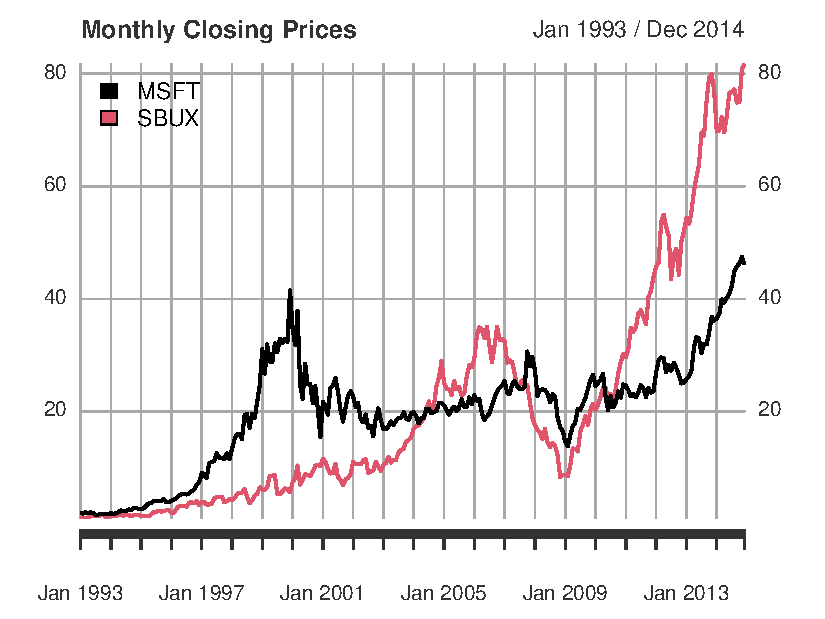
\includegraphics[width=0.8\textwidth,height=\textheight]{01-ReturnCalculations-new_files/figure-pdf/fig-MsftSbuxMonthlyPricesXts-1.pdf}

}

\caption{\label{fig-MsftSbuxMonthlyPricesXts}Single panel plot (default)
with \texttt{plot.xts()}}

\end{figure}

The default plot style in \texttt{plot.xts()} is a single-panel plot
with multiple series. You can also create multi-panel plots, as in
Figure Figure~\ref{fig-MsftSbuxPricesXtsMultiple}, by setting the
optional argument \texttt{multi.panel\ =\ TRUE} in the call to
\texttt{plot.xts()}

\begin{Shaded}
\begin{Highlighting}[]
\FunctionTok{plot}\NormalTok{(msftSbuxMonthlyPrices, }\AttributeTok{main=}\StringTok{"Monthly Closing Prices"}\NormalTok{, }
     \AttributeTok{multi.panel=}\ConstantTok{TRUE}\NormalTok{)}
\end{Highlighting}
\end{Shaded}

\begin{figure}[H]

{\centering 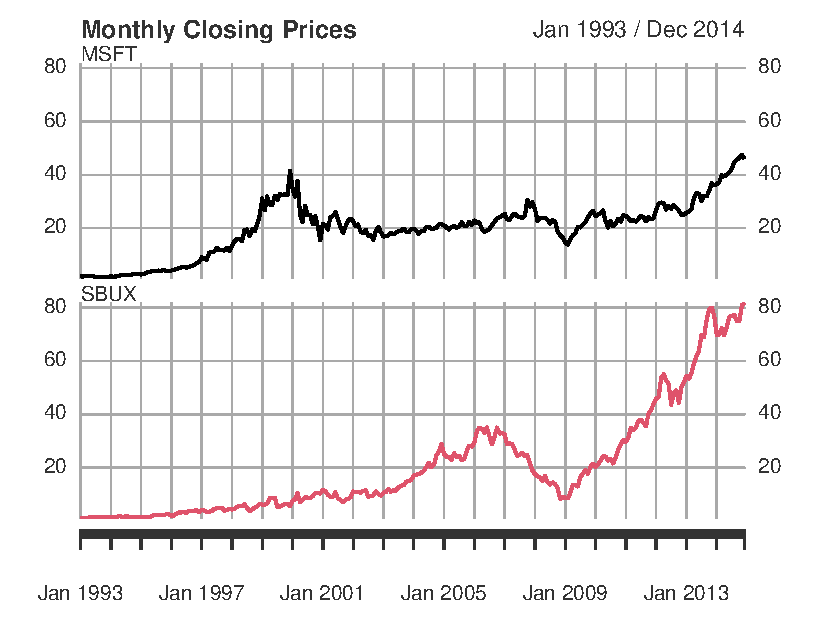
\includegraphics[width=0.8\textwidth,height=\textheight]{01-ReturnCalculations-new_files/figure-pdf/fig-MsftSbuxPricesXtsMultiple-1.pdf}

}

\caption{\label{fig-MsftSbuxPricesXtsMultiple}Multi-panel time series
plot with \texttt{plot.xts()}}

\end{figure}

See the help file for \texttt{plot.xts()} for more examples of plotting
\texttt{xts} objects.

Because the \texttt{xts} class inherits from the \texttt{zoo} class, the
\textbf{zoo} method function \texttt{plot.zoo()} can also be used to
plot \texttt{xts} objects. Figure Figure~\ref{fig-MsftSbuxPricesZoo} is
created with

\begin{Shaded}
\begin{Highlighting}[]
\FunctionTok{plot.zoo}\NormalTok{(msftSbuxMonthlyPrices, }\AttributeTok{plot.type=}\StringTok{"single"}\NormalTok{, }
         \AttributeTok{main=}\StringTok{"Monthly Closing Prices"}\NormalTok{,         }
         \AttributeTok{lwd =} \DecValTok{2}\NormalTok{, }\AttributeTok{col=}\FunctionTok{c}\NormalTok{(}\StringTok{"black"}\NormalTok{, }\StringTok{"red"}\NormalTok{), }\AttributeTok{ylab=}\StringTok{"Price"}\NormalTok{) }
\FunctionTok{grid}\NormalTok{() }
\FunctionTok{legend}\NormalTok{(}\AttributeTok{x=}\StringTok{"topleft"}\NormalTok{, }\AttributeTok{legend=}\FunctionTok{colnames}\NormalTok{(msftSbuxMonthlyPrices),         }
      \AttributeTok{lwd =} \DecValTok{2}\NormalTok{, }\AttributeTok{col=}\FunctionTok{c}\NormalTok{(}\StringTok{"black"}\NormalTok{, }\StringTok{"red"}\NormalTok{))}
\end{Highlighting}
\end{Shaded}

\begin{figure}[H]

{\centering 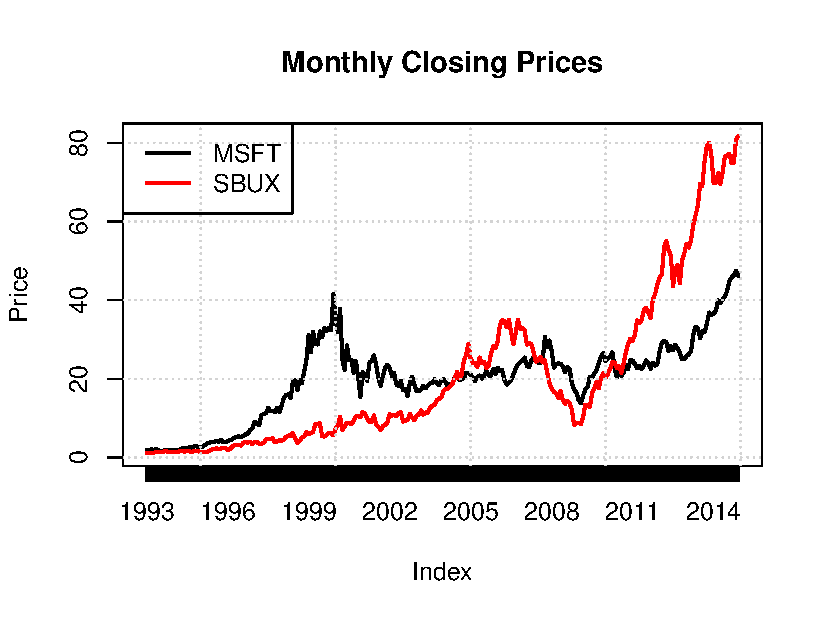
\includegraphics[width=0.8\textwidth,height=\textheight]{01-ReturnCalculations-new_files/figure-pdf/fig-MsftSbuxPricesZoo-1.pdf}

}

\caption{\label{fig-MsftSbuxPricesZoo}Single panel time series plot
(default) with \texttt{plot.zoo()}}

\end{figure}

A muti-panel plot, shown in Figure
Figure~\ref{fig-MsftSbuxPricesZooMultiple}, can be created using

\begin{Shaded}
\begin{Highlighting}[]
\FunctionTok{plot.zoo}\NormalTok{(msftSbuxMonthlyPrices, }\AttributeTok{plot.type=}\StringTok{"multiple"}\NormalTok{, }\AttributeTok{main=}\StringTok{""}\NormalTok{,}
         \AttributeTok{lwd =} \DecValTok{2}\NormalTok{, }\AttributeTok{col=}\FunctionTok{c}\NormalTok{(}\StringTok{"black"}\NormalTok{, }\StringTok{"red"}\NormalTok{), }\AttributeTok{cex.axis=}\FloatTok{0.8}\NormalTok{)}
\end{Highlighting}
\end{Shaded}

\begin{figure}[H]

{\centering 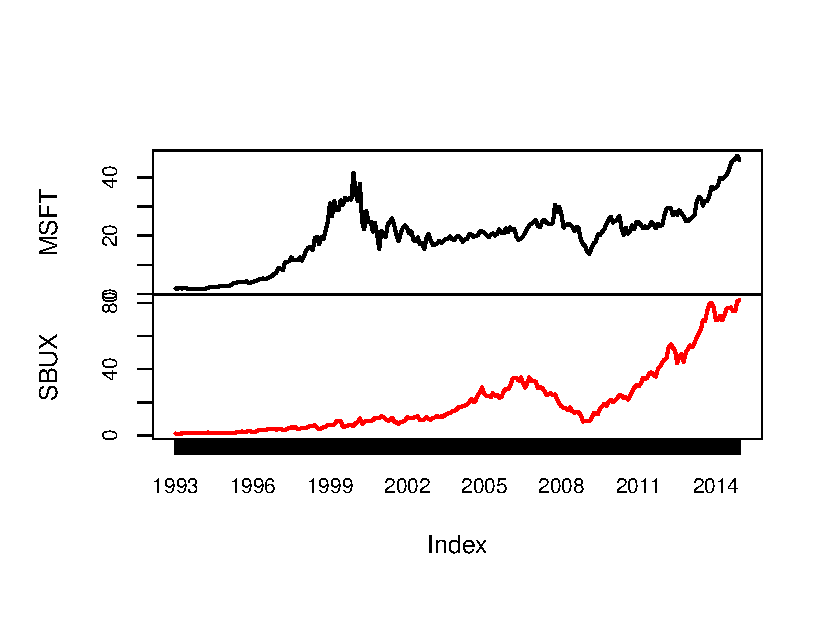
\includegraphics[width=0.8\textwidth,height=\textheight]{01-ReturnCalculations-new_files/figure-pdf/fig-MsftSbuxPricesZooMultiple-1.pdf}

}

\caption{\label{fig-MsftSbuxPricesZooMultiple}Multi-panel time series
plot with \texttt{plot.zoo()}}

\end{figure}

Creating plots with \texttt{plot.zoo()} is a bit more involved than with
\texttt{plot.xts()}, as \texttt{plot.xts()} is newer. See the help file
for \texttt{plot.zoo()} for more examples.

\hypertarget{ploting-xts-objects-using-autoplot-from-ggplot2}{%
\subsubsection{\texorpdfstring{Ploting \texttt{xts} objects using
\texttt{autoplot()} from
\textbf{ggplot2}}{Ploting xts objects using autoplot() from ggplot2}}\label{ploting-xts-objects-using-autoplot-from-ggplot2}}

The plots created using \texttt{plot.xts()} and \texttt{plot.zoo()} are
created using the base graphics system in R. This allows for a lot of
flexibility but often the resulting plots do not look very exciting or
modern. In addition, these functions are not well suited for plotting
many time series together in a single plot.

Another very popular graphics system in R is provided by the
\textbf{ggplot2} package by Hadley Wickham of RStudio. For plotting
\texttt{xts} objects, especially with multiple columns (data series),
the \textbf{ggplot2} function \texttt{autoplot()} is especially
convenient and easy:

\begin{Shaded}
\begin{Highlighting}[]
\FunctionTok{autoplot}\NormalTok{(msftSbuxDailyPrices, }\AttributeTok{facets =} \ConstantTok{NULL}\NormalTok{) }\SpecialCharTok{+}
  \FunctionTok{ggtitle}\NormalTok{(}\StringTok{"Daily Closing Prices"}\NormalTok{) }\SpecialCharTok{+}
  \FunctionTok{ylab}\NormalTok{(}\StringTok{"Closing Price Per Share"}\NormalTok{) }\SpecialCharTok{+}
  \FunctionTok{xlab}\NormalTok{(}\StringTok{"Year"}\NormalTok{)}
\end{Highlighting}
\end{Shaded}

\begin{figure}[H]

{\centering 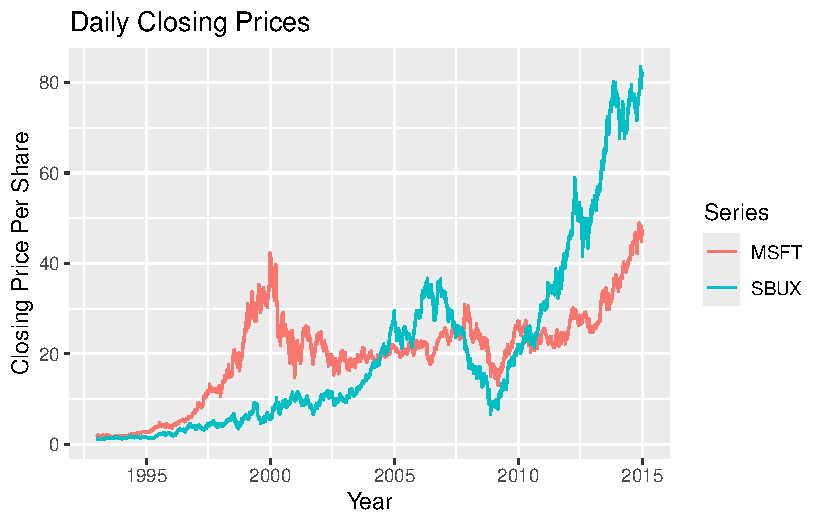
\includegraphics{01-ReturnCalculations-new_files/figure-pdf/unnamed-chunk-45-1.pdf}

}

\end{figure}

The syntax for creating graphs with \texttt{autoplot()} uses the
\emph{grammar of graphics} syntax from the \textbf{ggplot2} package. See
the \href{https://r-graphics.org/}{R Graphics Cookbook} for more details
and examples on using the \textbf{ggplot2} package. The call to
\texttt{autoplot()} first invokes the method function
\texttt{autoplot.zoo()} from the \textbf{zoo} package and creates a
basic time series plot. Additional layers showing a main title and axes
labels are added using \texttt{+}. The optional argument
\texttt{facets\ =\ NULL} specifies that all series are plotted together
on a single plot with different colors.

To produce a multi-panel plot call \texttt{autoplot()} with
\texttt{facets\ =\ Series\ \textasciitilde{}\ .}:

\begin{Shaded}
\begin{Highlighting}[]
\FunctionTok{autoplot}\NormalTok{(msftSbuxDailyPrices, }\AttributeTok{facets =}\NormalTok{ Series }\SpecialCharTok{\textasciitilde{}}\NormalTok{ .) }\SpecialCharTok{+}
  \FunctionTok{ggtitle}\NormalTok{(}\StringTok{"Daily Closing Prices"}\NormalTok{) }\SpecialCharTok{+}
  \FunctionTok{ylab}\NormalTok{(}\StringTok{"Closing Price Per Share"}\NormalTok{) }\SpecialCharTok{+}
  \FunctionTok{xlab}\NormalTok{(}\StringTok{"Year"}\NormalTok{)}
\end{Highlighting}
\end{Shaded}

\begin{figure}[H]

{\centering 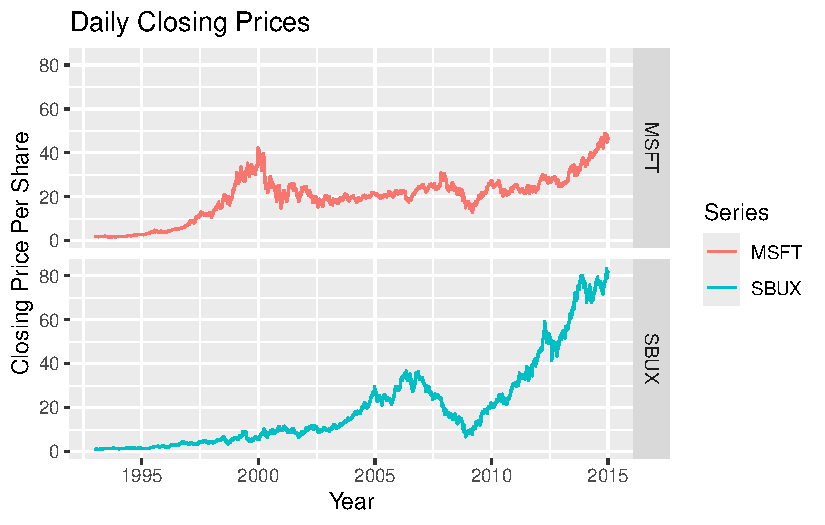
\includegraphics{01-ReturnCalculations-new_files/figure-pdf/unnamed-chunk-46-1.pdf}

}

\end{figure}

See the help file for \texttt{autoplot.zoo()} for more examples.

\hypertarget{calculating-returns}{%
\subsection{Calculating returns}\label{calculating-returns}}

In this sub-section, we illustrate how to calculate a time series of
returns from a time series of prices.

\hypertarget{brute-force-return-calculations}{%
\subsubsection{Brute force return
calculations}\label{brute-force-return-calculations}}

Consider computing simple monthly returns,
\(R_{t}=\frac{P_{t}-P_{t-1}}{P_{t-1}}\), from historical prices using
the \texttt{xts} object \texttt{sbuxMonthlyPrices}. The R code for a
brute force calculation is:

\begin{Shaded}
\begin{Highlighting}[]
\NormalTok{sbuxMonthlyReturns }\OtherTok{=} \FunctionTok{diff}\NormalTok{(sbuxMonthlyPrices)}\SpecialCharTok{/}\NormalTok{stats}\SpecialCharTok{::}\FunctionTok{lag}\NormalTok{(sbuxMonthlyPrices)}
\FunctionTok{head}\NormalTok{(sbuxMonthlyReturns, }\AttributeTok{n=}\DecValTok{3}\NormalTok{)}
\CommentTok{\#\textgreater{}             SBUX}
\CommentTok{\#\textgreater{} Jan 1993      NA}
\CommentTok{\#\textgreater{} Feb 1993 {-}0.0625}
\CommentTok{\#\textgreater{} Mar 1993  0.0476}
\end{Highlighting}
\end{Shaded}

Here, the \texttt{diff()} function computes the first difference in the
prices, \(P_{t}-P_{t-1}\), and the \texttt{lag()} function computes the
lagged price, \(P_{t-1}.\)\footnote{The method function
  \texttt{lag.xts()} works differently than generic \texttt{lag()}
  function and the method function \texttt{lag.zoo()}. In particular,
  \texttt{lag.xts()} with optional argument \texttt{k=1} gives the same
  result as \texttt{lag()} and \texttt{lag.zoo()} with \texttt{k=-1}.}
An equivalent calculation is \(R_{t}=\frac{P_{t}}{P_{t-1}}-1\):

\begin{Shaded}
\begin{Highlighting}[]
\FunctionTok{head}\NormalTok{(sbuxMonthlyPrices}\SpecialCharTok{/}\NormalTok{stats}\SpecialCharTok{::}\FunctionTok{lag}\NormalTok{(sbuxMonthlyPrices) }\SpecialCharTok{{-}} \DecValTok{1}\NormalTok{, }\AttributeTok{n=}\DecValTok{3}\NormalTok{)}
\CommentTok{\#\textgreater{}             SBUX}
\CommentTok{\#\textgreater{} Jan 1993      NA}
\CommentTok{\#\textgreater{} Feb 1993 {-}0.0625}
\CommentTok{\#\textgreater{} Mar 1993  0.0476}
\end{Highlighting}
\end{Shaded}

Notice that the return for January, 1993 is \texttt{NA} (missing value).
To automatically remove this missing value, use the R function
\texttt{na.omit()} or explicitly exclude the first observation:

\begin{Shaded}
\begin{Highlighting}[]
\FunctionTok{head}\NormalTok{(}\FunctionTok{na.omit}\NormalTok{(sbuxMonthlyReturns), }\AttributeTok{n=}\DecValTok{3}\NormalTok{)}
\CommentTok{\#\textgreater{}             SBUX}
\CommentTok{\#\textgreater{} Feb 1993 {-}0.0625}
\CommentTok{\#\textgreater{} Mar 1993  0.0476}
\CommentTok{\#\textgreater{} Apr 1993  0.0182}
\end{Highlighting}
\end{Shaded}

\begin{Shaded}
\begin{Highlighting}[]
\FunctionTok{head}\NormalTok{(sbuxMonthlyReturns[}\SpecialCharTok{{-}}\DecValTok{1}\NormalTok{], }\AttributeTok{n=}\DecValTok{3}\NormalTok{)}
\CommentTok{\#\textgreater{}             SBUX}
\CommentTok{\#\textgreater{} Feb 1993 {-}0.0625}
\CommentTok{\#\textgreater{} Mar 1993  0.0476}
\CommentTok{\#\textgreater{} Apr 1993  0.0182}
\end{Highlighting}
\end{Shaded}

To compute continuously compounded returns from simple returns, use:

\begin{Shaded}
\begin{Highlighting}[]
\NormalTok{sbuxMonthlyReturnsC }\OtherTok{=} \FunctionTok{na.omit}\NormalTok{(}\FunctionTok{log}\NormalTok{(}\DecValTok{1} \SpecialCharTok{+}\NormalTok{ sbuxMonthlyReturns))}
\FunctionTok{head}\NormalTok{(sbuxMonthlyReturnsC, }\AttributeTok{n=}\DecValTok{3}\NormalTok{)}
\CommentTok{\#\textgreater{}             SBUX}
\CommentTok{\#\textgreater{} Feb 1993 {-}0.0645}
\CommentTok{\#\textgreater{} Mar 1993  0.0465}
\CommentTok{\#\textgreater{} Apr 1993  0.0180}
\end{Highlighting}
\end{Shaded}

Or, equivalently, to compute continuously compounded returns directly
from prices, use:

\begin{Shaded}
\begin{Highlighting}[]
\NormalTok{sbuxMonthlyReturnsC }\OtherTok{=} \FunctionTok{na.omit}\NormalTok{(}\FunctionTok{diff}\NormalTok{(}\FunctionTok{log}\NormalTok{(sbuxMonthlyPrices))) }
\FunctionTok{head}\NormalTok{(sbuxMonthlyReturnsC, }\AttributeTok{n=}\DecValTok{3}\NormalTok{)}
\CommentTok{\#\textgreater{}             SBUX}
\CommentTok{\#\textgreater{} Feb 1993 {-}0.0645}
\CommentTok{\#\textgreater{} Mar 1993  0.0465}
\CommentTok{\#\textgreater{} Apr 1993  0.0180}
\end{Highlighting}
\end{Shaded}

The above calculations used an \texttt{xts} object with a single column.
If an \texttt{xts} object has multiple columns the same calculations
work for each column. For example,

\begin{Shaded}
\begin{Highlighting}[]
\NormalTok{msftSbuxMonthlyReturns }\OtherTok{=} \FunctionTok{diff}\NormalTok{(msftSbuxMonthlyPrices)}\SpecialCharTok{/}\NormalTok{stats}\SpecialCharTok{::}\FunctionTok{lag}\NormalTok{(msftSbuxMonthlyPrices)}
\FunctionTok{head}\NormalTok{(msftSbuxMonthlyReturns, }\AttributeTok{n=}\DecValTok{3}\NormalTok{)}
\CommentTok{\#\textgreater{}             MSFT    SBUX}
\CommentTok{\#\textgreater{} Jan 1993      NA      NA}
\CommentTok{\#\textgreater{} Feb 1993 {-}0.0365 {-}0.0625}
\CommentTok{\#\textgreater{} Mar 1993  0.1135  0.0476}
\end{Highlighting}
\end{Shaded}

Also,

\begin{Shaded}
\begin{Highlighting}[]
\NormalTok{msftSbuxMonthlyReturnsC }\OtherTok{=} \FunctionTok{diff}\NormalTok{(}\FunctionTok{log}\NormalTok{(msftSbuxMonthlyPrices))}
\FunctionTok{head}\NormalTok{(msftSbuxMonthlyReturnsC, }\AttributeTok{n=}\DecValTok{3}\NormalTok{)}
\CommentTok{\#\textgreater{}             MSFT    SBUX}
\CommentTok{\#\textgreater{} Jan 1993      NA      NA}
\CommentTok{\#\textgreater{} Feb 1993 {-}0.0371 {-}0.0645}
\CommentTok{\#\textgreater{} Mar 1993  0.1075  0.0465}
\end{Highlighting}
\end{Shaded}

These are examples of \emph{vectorized} calculations. That is, the
calculations are performed on all columns simultaneously. This is
computationally more efficient than looping the same calculation for
each column. In R, you should try to vectorize calculations whenever
possible.

\hypertarget{calculating-returns-using-return.calculate}{%
\subsubsection{\texorpdfstring{Calculating returns using
\texttt{Return.calculate()}}{Calculating returns using Return.calculate()}}\label{calculating-returns-using-return.calculate}}

Simple and continuously compounded returns can be computed using the
\textbf{PerformanceAnalytics} function \texttt{Return.calculate()}:

\begin{Shaded}
\begin{Highlighting}[]
\CommentTok{\# Simple returns}
\NormalTok{sbuxMonthlyReturns }\OtherTok{=} \FunctionTok{Return.calculate}\NormalTok{(sbuxMonthlyPrices) }
\FunctionTok{head}\NormalTok{(sbuxMonthlyReturns, }\AttributeTok{n=}\DecValTok{3}\NormalTok{)}
\CommentTok{\#\textgreater{}             SBUX}
\CommentTok{\#\textgreater{} Jan 1993      NA}
\CommentTok{\#\textgreater{} Feb 1993 {-}0.0625}
\CommentTok{\#\textgreater{} Mar 1993  0.0476}
\end{Highlighting}
\end{Shaded}

\begin{Shaded}
\begin{Highlighting}[]
\CommentTok{\# CC returns }
\NormalTok{sbuxMonthlyReturnsC }\OtherTok{=} \FunctionTok{Return.calculate}\NormalTok{(sbuxMonthlyPrices, }\AttributeTok{method=}\StringTok{"log"}\NormalTok{) }
\FunctionTok{head}\NormalTok{(sbuxMonthlyReturnsC, }\AttributeTok{n=}\DecValTok{3}\NormalTok{)}
\CommentTok{\#\textgreater{}             SBUX}
\CommentTok{\#\textgreater{} Jan 1993      NA}
\CommentTok{\#\textgreater{} Feb 1993 {-}0.0645}
\CommentTok{\#\textgreater{} Mar 1993  0.0465}
\end{Highlighting}
\end{Shaded}

\texttt{Return.calculate()} also works with \texttt{xts} objects with
multiple columns:

\begin{Shaded}
\begin{Highlighting}[]
\NormalTok{msftSbuxMonthlyReturns }\OtherTok{=} \FunctionTok{Return.calculate}\NormalTok{(msftSbuxMonthlyPrices)}
\FunctionTok{head}\NormalTok{(msftSbuxMonthlyReturns, }\DecValTok{3}\NormalTok{)}
\CommentTok{\#\textgreater{}             MSFT    SBUX}
\CommentTok{\#\textgreater{} Jan 1993      NA      NA}
\CommentTok{\#\textgreater{} Feb 1993 {-}0.0365 {-}0.0625}
\CommentTok{\#\textgreater{} Mar 1993  0.1135  0.0476}
\end{Highlighting}
\end{Shaded}

The advantages of using \texttt{Return.calculate()} instead of brute
force calculations are: (1) clarity of code (you know what is being
computed), (2) the same function is used for both simple and
continuously compounded returns, (3) built-in error checking.

\hypertarget{equity-curves}{%
\subsubsection{Equity curves}\label{equity-curves}}

\index{Equity curves} To directly compare the investment performance of
two or more assets, plot the simple multi-period cumulative returns of
each asset on the same graph. This type of graph, sometimes called an
\emph{equity curve}, shows how a one dollar investment amount in each
asset grows over time. Better performing assets have higher equity
curves. For simple returns, the \emph{k}-period returns are
\(R_{t}(k)=\prod\limits _{j=0}^{k-1}(1+R_{t-j})\) and represent the
growth of one dollar invested for \(k\) periods. For continuously
compounded returns, the \emph{k}-period returns are
\(r_{t}(k)=\sum\limits _{j=0}^{k-1}r_{t-j}\). However, this continuously
compounded \(k\)-period return must be converted to a simple
\(k\)-period return, using \(R_{t}(k)=\exp\left(r_{t}(k)\right)-1\), to
properly represent the growth of one dollar invested for \(k\) periods.

\begin{example}[Equity curves for Microsoft and Starbucks monthly
returns]\protect\hypertarget{exm-example0506}{}\label{exm-example0506}

To create the equity curves for Microsoft and Starbucks based on simple
returns use (You can also use the \textbf{PerformanceAnalytics} function
\texttt{chart.CumReturns()})

\end{example}

\begin{Shaded}
\begin{Highlighting}[]
\NormalTok{msftMonthlyReturns }\OtherTok{=} \FunctionTok{na.omit}\NormalTok{(}\FunctionTok{Return.calculate}\NormalTok{(msftMonthlyPrices))}
\NormalTok{sbuxMonthlyReturns }\OtherTok{=} \FunctionTok{na.omit}\NormalTok{(}\FunctionTok{Return.calculate}\NormalTok{(sbuxMonthlyPrices))}
\NormalTok{equityCurveMsft }\OtherTok{=} \FunctionTok{cumprod}\NormalTok{(}\DecValTok{1} \SpecialCharTok{+}\NormalTok{ msftMonthlyReturns)  }
\NormalTok{equityCurveSbux }\OtherTok{=} \FunctionTok{cumprod}\NormalTok{(}\DecValTok{1} \SpecialCharTok{+}\NormalTok{ sbuxMonthlyReturns)  }
\NormalTok{dataToPlot }\OtherTok{=} \FunctionTok{merge}\NormalTok{(equityCurveMsft, equityCurveSbux)}
\FunctionTok{plot}\NormalTok{(dataToPlot, }\AttributeTok{main=}\StringTok{"Monthly Equity Curves"}\NormalTok{, }\AttributeTok{legend.loc=}\StringTok{"topleft"}\NormalTok{)}
\end{Highlighting}
\end{Shaded}

\begin{figure}[H]

{\centering 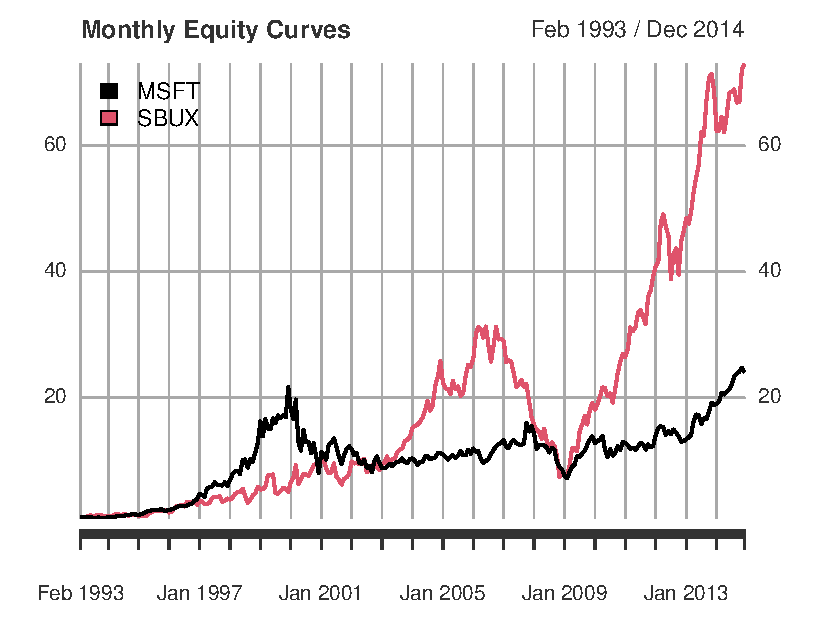
\includegraphics[width=0.8\textwidth,height=\textheight]{01-ReturnCalculations-new_files/figure-pdf/fig-DSmonthlyCumulativeReturns-1.pdf}

}

\caption{\label{fig-DSmonthlyCumulativeReturns}Monthly equity curve for
Microsoft and Starbucks.}

\end{figure}

The R function \texttt{cumprod()} creates the cumulative products needed
for the equity curves. Figure
Figure~\ref{fig-DSmonthlyCumulativeReturns} shows that a one dollar
investment in Starbucks dominated a one dollar investment in Microsoft
over the given period. In particular, \$1 invested in Microsoft grew to
about only \$22 (over about 20 years) whereas \$1 invested in Starbucks
grew over \$70. Notice the huge increases and decreases in value of
Microsoft during the dot-com bubble and bust over the period 1998 -
2001, and the enormous increase in value of Starbucks from 2009 - 2014.

\hfill{}\(\blacksquare\)

\hypertarget{calculating-portfolio-returns-from-time-series-data}{%
\subsection{Calculating portfolio returns from time series
data}\label{calculating-portfolio-returns-from-time-series-data}}

As discussed in sub-section
Section~\ref{sec-portfolios-and-portfolio-returns}, the calculation of
portfolio returns depends on the assumptions made about the portfolio
weights over time.

\hypertarget{constant-portfolio-weights-1}{%
\subsubsection{Constant portfolio
weights}\label{constant-portfolio-weights-1}}

The easiest case assumes that portfolio weights are constant over time.
To illustrate, consider an equally weighted portfolio of Microsoft and
Starbucks stock. A time series a portfolio monthly returns can be
created directly from the monthly returns on Microsoft and Starbucks
stock:

\begin{Shaded}
\begin{Highlighting}[]
\NormalTok{x.msft }\OtherTok{=}\NormalTok{ x.sbux }\OtherTok{=} \FloatTok{0.5}
\NormalTok{msftMonthlyReturns }\OtherTok{=} \FunctionTok{na.omit}\NormalTok{(}\FunctionTok{Return.calculate}\NormalTok{(msftMonthlyPrices))}
\NormalTok{sbuxMonthlyReturns }\OtherTok{=} \FunctionTok{na.omit}\NormalTok{(}\FunctionTok{Return.calculate}\NormalTok{(sbuxMonthlyPrices))}
\NormalTok{equalWeightPortMonthlyReturns }\OtherTok{=}\NormalTok{ x.msft}\SpecialCharTok{*}\NormalTok{msftMonthlyReturns }\SpecialCharTok{+} 
\NormalTok{  x.sbux}\SpecialCharTok{*}\NormalTok{sbuxMonthlyReturns}
\FunctionTok{head}\NormalTok{(equalWeightPortMonthlyReturns, }\DecValTok{3}\NormalTok{)}
\CommentTok{\#\textgreater{}             MSFT}
\CommentTok{\#\textgreater{} Feb 1993 {-}0.0495}
\CommentTok{\#\textgreater{} Mar 1993  0.0806}
\CommentTok{\#\textgreater{} Apr 1993 {-}0.0297}
\end{Highlighting}
\end{Shaded}

The same calculation can be performed using the
\textbf{PerformanceAnalytics} function \texttt{Return.portfolio()}:

\begin{Shaded}
\begin{Highlighting}[]
\NormalTok{equalWeightPortMonthlyReturns }\OtherTok{=} 
  \FunctionTok{Return.portfolio}\NormalTok{(}\FunctionTok{na.omit}\NormalTok{(msftSbuxMonthlyReturns), }
                   \AttributeTok{weights =} \FunctionTok{c}\NormalTok{(x.msft, x.sbux),}
                   \AttributeTok{rebalance\_on =} \StringTok{"months"}\NormalTok{)}
\FunctionTok{head}\NormalTok{(equalWeightPortMonthlyReturns, }\DecValTok{3}\NormalTok{)}
\CommentTok{\#\textgreater{}          portfolio.returns}
\CommentTok{\#\textgreater{} Feb 1993           {-}0.0495}
\CommentTok{\#\textgreater{} Mar 1993            0.0806}
\CommentTok{\#\textgreater{} Apr 1993           {-}0.0297}
\end{Highlighting}
\end{Shaded}

Here, the optional argument \texttt{rebalance\_on\ =\ "months"}
specifies that the portfolio is to be rebalanced to the specified
weights at the beginning of every month.

If you also want the asset contributions to the portfolio return set the
optional argument \texttt{contribution\ =\ TRUE} (recall, asset
contributions sum to the portfolio return):

\begin{Shaded}
\begin{Highlighting}[]
\NormalTok{equalWeightPortMonthlyReturns }\OtherTok{=} 
  \FunctionTok{Return.portfolio}\NormalTok{(}\FunctionTok{na.omit}\NormalTok{(msftSbuxMonthlyReturns),}
                   \AttributeTok{weights =} \FunctionTok{c}\NormalTok{(x.msft, x.sbux),}
                   \AttributeTok{rebalance\_on =} \StringTok{"months"}\NormalTok{,}
                   \AttributeTok{contribution =} \ConstantTok{TRUE}\NormalTok{)}
\FunctionTok{head}\NormalTok{(equalWeightPortMonthlyReturns, }\DecValTok{3}\NormalTok{)}
\CommentTok{\#\textgreater{}          portfolio.returns    MSFT     SBUX}
\CommentTok{\#\textgreater{} Feb 1993           {-}0.0495 {-}0.0182 {-}0.03125}
\CommentTok{\#\textgreater{} Mar 1993            0.0806  0.0568  0.02381}
\CommentTok{\#\textgreater{} Apr 1993           {-}0.0297 {-}0.0388  0.00909}
\end{Highlighting}
\end{Shaded}

You can see the rebalancing calculations by setting the optional
argument \texttt{verbose\ =\ TRUE}:

\begin{Shaded}
\begin{Highlighting}[]
\NormalTok{equalWeightPortMonthlyReturns }\OtherTok{=} 
  \FunctionTok{Return.portfolio}\NormalTok{(}\FunctionTok{na.omit}\NormalTok{(msftSbuxMonthlyReturns),}
                   \AttributeTok{weights =} \FunctionTok{c}\NormalTok{(x.msft, x.sbux),}
                   \AttributeTok{rebalance\_on =} \StringTok{"months"}\NormalTok{,}
                   \AttributeTok{verbose =} \ConstantTok{TRUE}\NormalTok{)}
\FunctionTok{names}\NormalTok{(equalWeightPortMonthlyReturns)}
\CommentTok{\#\textgreater{} [1] "returns"      "contribution" "BOP.Weight"   "EOP.Weight"   "BOP.Value"   }
\CommentTok{\#\textgreater{} [6] "EOP.Value"}
\end{Highlighting}
\end{Shaded}

In this case \texttt{Return.portfolio()} returns a list with the above
components. The component \texttt{BOP.Weight} shows the
beginning-of-period portfolio weights, and the component
\texttt{EOP.Weight} shows the end-of-period portfolio weights (before
any rebalancing).

\begin{Shaded}
\begin{Highlighting}[]
\FunctionTok{head}\NormalTok{(equalWeightPortMonthlyReturns}\SpecialCharTok{$}\NormalTok{BOP.Weight, }\DecValTok{3}\NormalTok{)}
\CommentTok{\#\textgreater{}          MSFT SBUX}
\CommentTok{\#\textgreater{} Feb 1993  0.5  0.5}
\CommentTok{\#\textgreater{} Mar 1993  0.5  0.5}
\CommentTok{\#\textgreater{} Apr 1993  0.5  0.5}
\end{Highlighting}
\end{Shaded}

With monthly returns and with \texttt{rebalance\_on\ =\ "months"}, the
beginning-of-period weights are always rebalanced to the initially
supplied weights.

\begin{Shaded}
\begin{Highlighting}[]
\FunctionTok{head}\NormalTok{(equalWeightPortMonthlyReturns}\SpecialCharTok{$}\NormalTok{EOP.Weight, }\DecValTok{3}\NormalTok{)}
\CommentTok{\#\textgreater{}           MSFT  SBUX}
\CommentTok{\#\textgreater{} Feb 1993 0.507 0.493}
\CommentTok{\#\textgreater{} Mar 1993 0.515 0.485}
\CommentTok{\#\textgreater{} Apr 1993 0.475 0.525}
\end{Highlighting}
\end{Shaded}

Because the returns for Microsoft and Starbux are different every month
the end-of-period weights drift away from the beginning-of-period
weights.

\hypertarget{buy-and-hold-portfolio}{%
\subsubsection{Buy-and-hold portfolio}\label{buy-and-hold-portfolio}}

In the buy-and-hold portfolio, no rebalancing of the initial portfolio
is done and the portfolio weights are allowed to evolve over time based
on the returns of the assets. Hence, the computation of the portfolio
return each month requires knowing the weights on each asset each month.
You can use \texttt{Return.portfolio()} to compute the buy-and-hold
portfolio returns as follows:

\begin{Shaded}
\begin{Highlighting}[]
\NormalTok{buyHoldPortMonthlyReturns }\OtherTok{=} 
  \FunctionTok{Return.portfolio}\NormalTok{(}\FunctionTok{na.omit}\NormalTok{(msftSbuxMonthlyReturns),}
                   \AttributeTok{weights =} \FunctionTok{c}\NormalTok{(x.msft, x.sbux))}
\FunctionTok{head}\NormalTok{(buyHoldPortMonthlyReturns, }\DecValTok{3}\NormalTok{)}
\CommentTok{\#\textgreater{}          portfolio.returns}
\CommentTok{\#\textgreater{} Feb 1993           {-}0.0495}
\CommentTok{\#\textgreater{} Mar 1993            0.0810}
\CommentTok{\#\textgreater{} Apr 1993           {-}0.0319}
\end{Highlighting}
\end{Shaded}

Omitting the optional argument \texttt{rebalance\_on} tells
\texttt{Return.portfolio()} to not rebalance the portfolio at all
(default behavior of the function).

\hypertarget{periodic-rebalancing}{%
\subsubsection{Periodic rebalancing}\label{periodic-rebalancing}}

In practice, a portfolio may be rebalanced at a specific frequency that
is different than the frequency of the returns. For example, with
monthly returns the portfolio might be rebalanced quarterly or annually.
For example, to rebalance the equally weighted portfolio of Microsoft
and Starbucks stock each quarter (every three months) use

\begin{Shaded}
\begin{Highlighting}[]
\NormalTok{equalWeightQtrPortMonthlyReturns }\OtherTok{=} 
  \FunctionTok{Return.portfolio}\NormalTok{(}\FunctionTok{na.omit}\NormalTok{(msftSbuxMonthlyReturns),}
                   \AttributeTok{weights =} \FunctionTok{c}\NormalTok{(x.msft, x.sbux),}
                   \AttributeTok{rebalance\_on =} \StringTok{"quarters"}\NormalTok{)}
\FunctionTok{head}\NormalTok{(equalWeightQtrPortMonthlyReturns, }\DecValTok{3}\NormalTok{)}
\CommentTok{\#\textgreater{}          portfolio.returns}
\CommentTok{\#\textgreater{} Feb 1993           {-}0.0495}
\CommentTok{\#\textgreater{} Mar 1993            0.0810}
\CommentTok{\#\textgreater{} Apr 1993           {-}0.0297}
\end{Highlighting}
\end{Shaded}

In between quarters, the portfolio evolves as a buy-and-hold portfolio.
To see the details of the rebalancing set \texttt{verbose\ =\ TRUE} in
the call to \texttt{Return.Portfolio()}.

\hypertarget{active-portfolio-weights}{%
\subsubsection{Active portfolio
weights}\label{active-portfolio-weights}}

If the weights are actively chosen at specific time periods, these
weights can be supplied to the function \texttt{Return.portfolio()} to
compute the portfolio return.

\hypertarget{downloading-financial-data-from-the-internet}{%
\subsection{Downloading financial data from the
internet}\label{downloading-financial-data-from-the-internet}}

The data for the examples in this book, available in the
\textbf{introcompFinr} package, were downloaded from
\href{https://finance.yahoo.com/}{finance.yahoo.com} using the
\texttt{getSymbols()} function from the \index{quantmod}
\textbf{quantmod} package.

For example, to download daily data on Amazon and Google stock (ticker
symbols AMZN and GOOG) from January 3, 2007 through January 3, 2020 use
\texttt{getSymbols()} as follows:

\begin{Shaded}
\begin{Highlighting}[]
\FunctionTok{options}\NormalTok{(}\StringTok{"getSymbols.warning4.0"}\OtherTok{=}\ConstantTok{FALSE}\NormalTok{)}
\FunctionTok{suppressPackageStartupMessages}\NormalTok{(}\FunctionTok{library}\NormalTok{(quantmod))}
\FunctionTok{getSymbols}\NormalTok{(}\AttributeTok{Symbols =} \FunctionTok{c}\NormalTok{(}\StringTok{"AMZN"}\NormalTok{, }\StringTok{"GOOG"}\NormalTok{), }\AttributeTok{from=}\StringTok{"2007{-}01{-}03"}\NormalTok{, }\AttributeTok{to=}\StringTok{"2020{-}01{-}03"}\NormalTok{,}
           \AttributeTok{auto.assign=}\ConstantTok{TRUE}\NormalTok{, }\AttributeTok{warnings=}\ConstantTok{FALSE}\NormalTok{)}
\CommentTok{\#\textgreater{} [1] "AMZN" "GOOG"}
\FunctionTok{class}\NormalTok{(AMZN)}
\CommentTok{\#\textgreater{} [1] "xts" "zoo"}
\end{Highlighting}
\end{Shaded}

The \texttt{xts} objects \texttt{AMZN} and \texttt{GOOG} each have six
columns containing the daily open price for the day, high price for the
day, low price for the day, close price for the day, volume for the day,
and (dividend and split) adjusted closing price for the day:

\begin{Shaded}
\begin{Highlighting}[]
\FunctionTok{head}\NormalTok{(AMZN, }\DecValTok{3}\NormalTok{)}
\CommentTok{\#\textgreater{}            AMZN.Open AMZN.High AMZN.Low AMZN.Close AMZN.Volume AMZN.Adjusted}
\CommentTok{\#\textgreater{} 2007{-}01{-}03      1.93      1.95     1.90       1.93    2.48e+08          1.93}
\CommentTok{\#\textgreater{} 2007{-}01{-}04      1.93      1.96     1.91       1.95    1.26e+08          1.95}
\CommentTok{\#\textgreater{} 2007{-}01{-}05      1.94      1.94     1.88       1.92    1.32e+08          1.92}
\end{Highlighting}
\end{Shaded}

\begin{Shaded}
\begin{Highlighting}[]
\FunctionTok{head}\NormalTok{(GOOG, }\DecValTok{3}\NormalTok{)}
\CommentTok{\#\textgreater{}            GOOG.Open GOOG.High GOOG.Low GOOG.Close GOOG.Volume GOOG.Adjusted}
\CommentTok{\#\textgreater{} 2007{-}01{-}03      11.6      11.9     11.5       11.6    3.09e+08          11.5}
\CommentTok{\#\textgreater{} 2007{-}01{-}04      11.7      12.1     11.7       12.0    3.17e+08          11.9}
\CommentTok{\#\textgreater{} 2007{-}01{-}05      12.0      12.1     11.9       12.1    2.76e+08          12.0}
\end{Highlighting}
\end{Shaded}

\hypertarget{further-reading-return-calculations}{%
\section{Further Reading: Return
Calculations}\label{further-reading-return-calculations}}

This chapter describes basic asset return calculations with an emphasis
on equity calculations. Similar material is covered in Chapter 2 of
(Ruppert and Matteson 2015). Comprehensive coverage of general return
calculations is given in (Bacon 2008) and (Christopherson, Carino, and
Ferson 2009). The virtues of portfolio rebalancing are discussed in
(\textbf{Ang-2014?}) and (\textbf{Qian-2019?}).

This chapter introduced you to the R packages
\textbf{PerformanceAnalytics}, \textbf{quantmod}, and \textbf{xts} for
working with financial time series. It is recommended to read the
vignettes included in each of these packages. Jeff Ryan's original
\href{http://www.quantmod.com/}{quantmod page}, while a bit outdated,
has many useful examples of working with \textbf{quantmod} and
\textbf{xts}. A good
\href{http://joshuaulrich.github.io/xts/index.html}{online tutorial} for
the \textbf{xts} package is provided by Joshua Ulrich, one of the
creators of \textbf{xts}.

There are many useful R packages for the analysis of financial data. An
up-to-date list of R packages relevant for finance is given on the
\href{https://cran.r-project.org/web/views/Finance.html}{Empirical
Finance Task View} on the comprehensive R archive network (CRAN).

\newpage{}

\hypertarget{appendix-properties-of-exponentials-and-logarithms}{%
\section{Appendix: Properties of Exponentials and
Logarithms}\label{appendix-properties-of-exponentials-and-logarithms}}

The computation of continuously compounded returns requires the use of
natural logarithms. The natural logarithm function, \(\ln(\cdot),\) is
the inverse of the exponential function, \(e^{(\cdot)}=\exp(\cdot),\)
where \(e^{1}=2.718.\) That is, \(\ln(x)\) is defined such that
\(x=\ln(e^{x}).\) Figure Figure~\ref{fig-logexp} plots \(e^{x}\) and
\(\ln(x)\). Notice that \(e^{x}\) is always positive and increasing in
\(x\). \(\ln(x)\) is monotonically increasing in \(x\) and is only
defined for \(x>0.\) Also note that \(\ln(1)=0\) and \(\ln(0)=-\infty.\)

\begin{figure}

{\centering 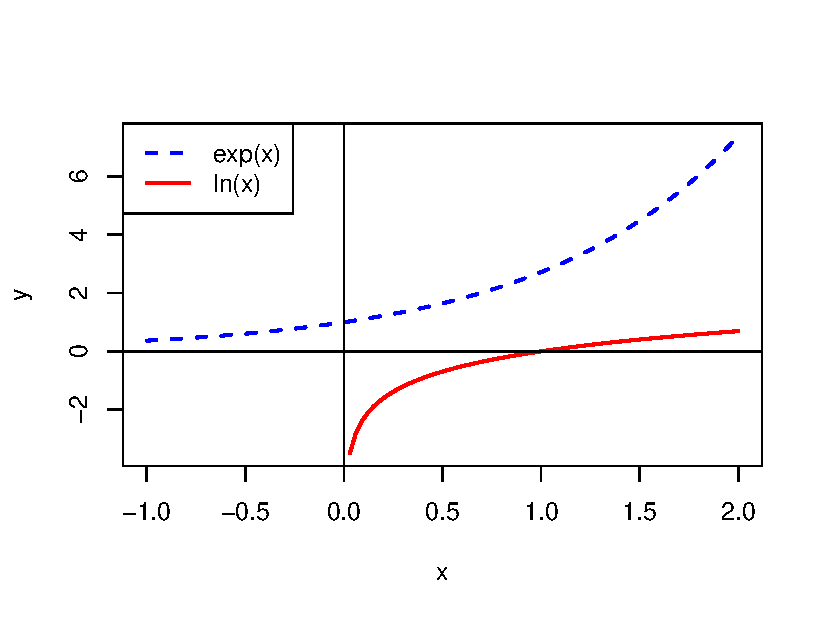
\includegraphics[width=0.8\textwidth,height=\textheight]{01-ReturnCalculations-new_files/figure-pdf/fig-logexp-1.pdf}

}

\caption{\label{fig-logexp}Exponential and natural logarithm functions.}

\end{figure}

The exponential and natural logarithm functions have the following
properties:

\begin{enumerate}
\def\labelenumi{\arabic{enumi}.}
\tightlist
\item
  \(\ln(x\cdot y)=\ln(x)+\ln(y),\) \(x,y>0\)
\item
  \(\ln(x/y)=\ln(x)-\ln(y),\) \(x,y>0\)
\item
  \(\ln(x^{y})=y\ln(x),\) \(x>0\)
\item
  \(\frac{d\ln(x)}{dx}=\frac{1}{x},\) \(x>0\)
\item
  \(\frac{d}{dx}\ln(f(x))=\frac{1}{f(x)}\frac{d}{dx}f(x)\) (chain-rule)
\item
  \(e^{x}e^{y}=e^{x+y}\)
\item
  \(e^{x}e^{-y}=e^{x-y}\)
\item
  \((e^{x})^{y}=e^{xy}\)
\item
  \(e^{\ln(x)}=x\)
\item
  \(\frac{d}{dx}e^{x}=e^{x}\)
\item
  \(\frac{d}{dx}e^{f(x)}=e^{f(x)}\frac{d}{dx}f(x)\) (chain-rule)
\end{enumerate}

\newpage{}

\hypertarget{exercises}{%
\section{Exercises}\label{exercises}}

\hypertarget{analytical-problems}{%
\subsection*{Analytical Problems}\label{analytical-problems}}
\addcontentsline{toc}{subsection}{Analytical Problems}

\begin{exercise}[]\protect\hypertarget{exr-exercise0101}{}\label{exr-exercise0101}

In this question you will see how the future value of an investment,
\(FV_n\) varies with the interest rate, \(R\), and the investment
horizon, \(n\). Let the initial amount invested be \(V=\$1,000\). For a
grid of values \(R=0.01, 0.02, \ldots , 0.10\) and \(n=1,2,\ldots 10\),
compute and plot \(FV_n\).

\end{exercise}

\begin{exercise}[]\protect\hypertarget{exr-exercise0102}{}\label{exr-exercise0102}

Consider the following credit card offer from a hypothetical bank. The
card advertises an annual percentage rate (APR) of \(19.34\%\). However,
the bank actually compounds interest charges on a daily basis.

\begin{enumerate}
\def\labelenumi{\arabic{enumi}.}
\tightlist
\item
  Assuming 365 days in the year, what is the daily periodic interest
  rate being charged?
\item
  If you carried a \$1,000 balance throughout the year, how much would
  you owe at the end of the year?
\end{enumerate}

\end{exercise}

\begin{exercise}[]\protect\hypertarget{exr-exercise0103}{}\label{exr-exercise0103}

Consider ``payday loans''. Payday loans are short-term loans made to
consumers, often for less than two weeks, and are offered by companies
such as AmeriCash Advance and National Payday. The loan works like this:
You write a check today that is postdated and the company gives you an
amount of money less than the check. When the check date arrives, you go
to the store and pay cash for the check, or the company cashes the
check. For example, suppose AmeriCash Advance allows you to write a
postdated check for \$125 for 15 days later in return for a \$100 loan
today.

\begin{enumerate}
\def\labelenumi{\arabic{enumi}.}
\tightlist
\item
  What is the annual percentage rate (APR) on this loan?
\item
  What is the effective annual rate (EAR)?
\end{enumerate}

\end{exercise}

\begin{exercise}[]\protect\hypertarget{exr-exercise0104}{}\label{exr-exercise0104}

Consider the following (actual) monthly adjusted closing price data for
Starbucks stock over the period December 2004 through December 2005

\begin{longtable}[]{@{}lr@{}}
\caption{End of Month Price Data for Starbucks Stock}\tabularnewline
\toprule\noalign{}
Date & Price \\
\midrule\noalign{}
\endfirsthead
\toprule\noalign{}
Date & Price \\
\midrule\noalign{}
\endhead
\bottomrule\noalign{}
\endlastfoot
December, 2004 & 31.2 \\
January, 2005 & 27.0 \\
February, 2005 & 25.9 \\
March, 2005 & 25.8 \\
April, 2005 & 24.8 \\
May, 2005 & 27.4 \\
June, 2005 & 25.8 \\
July, 2005 & 26.3 \\
August, 2005 & 24.5 \\
September, 2005 & 25.1 \\
October, 2005 & 28.3 \\
November, 2005 & 30.4 \\
December, 2005 & 30.5 \\
\end{longtable}

For the following questions, first do the return calculations by hand.
That is, give the appropriate return calculation formula and evaluate
the result. Then, check your hand calculations using the corresponding R
calculations.

\begin{enumerate}
\def\labelenumi{\arabic{enumi}.}
\tightlist
\item
  Using the data in the table, what is the simple monthly return between
  the end of December 2004 and the end of January 2005? If you invested
  \$10,000 in Starbucks at the end of December 2004, how much would the
  investment be worth at the end of January 2005?
\item
  Using the data in the table, what is the continuously compounded
  monthly return between December 2004 and January 2005? Convert this
  continuously compounded return to a simple return (you should get the
  same answer as in part 1).
\item
  Assuming that the simple monthly return you computed in part 1 is the
  same for 12 months, what is the annual return with monthly
  compounding?
\item
  Assuming that the continuously compounded monthly return you computed
  in part 2 is the same for 12 months, what is the continuously
  compounded annual return?
\item
  Using the data in the table, compute the actual simple annual return
  between December 2004 and December 2005. If you invested \$10,000 in
  Starbucks at the end of December 2004, how much would the investment
  be worth at the end of December 2005? Compare with your result in part
  3.
\item
  Using the data in the table, compute the actual annual continuously
  compounded return between December 2004 and December 2005. Compare
  with your result in part 4. Convert this continuously compounded
  return to a simple return (you should get the same answer as in part
  5).
\end{enumerate}

\end{exercise}

\begin{exercise}[]\protect\hypertarget{exr-exercise0105}{}\label{exr-exercise0105}

Consider a one month investment in two Northwest stocks: Amazon and
Costco. Suppose you buy Amazon and Costco at the end of September at
\(P_{A,t-1}=\$38.23\), \(P_{C,t-1}=\$41.11\) and then sell at the end of
the October for \(P_{A,t}=\$41.29\) and \(P_{C,t}=\$41.74\). (Note:
these are actual closing prices for 2004 taken from Yahoo!)

For the following questions, first do the return calculations by hand.
That is, give the appropriate return calculation formula and evaluate
the result. Then, check your hand calculations using the corresponding R
calculations.

\begin{enumerate}
\def\labelenumi{\arabic{enumi}.}
\tightlist
\item
  What are the simple monthly returns for the two stocks?
\item
  What are the continuously compounded returns for the two stocks?
\item
  Suppose Costco paid a \$0.10 per share cash dividend at the end of
  October. What is the monthly simple total return on Costco? What is
  the monthly dividend yield?
\item
  Suppose the monthly returns on Amazon and Costco from part 1 above are
  the same every month for 1 year. Compute the simple annual returns as
  well as the continuously compounded annual returns for the two stocks.
\item
  At the end of September 2004, suppose you have \$10,000 to invest in
  Amazon and Costco over the next month. If you invest \$8000 in Amazon
  and \$2000 in Costco, what are your portfolio shares, \(x_{A}\) and
  \(x_{C}\)?
\item
  Continuing with part 5, compute the monthly simple return and the
  monthly continuously compounded return on the portfolio. Assume that
  Costco does not pay a dividend.
\end{enumerate}

\end{exercise}

\begin{exercise}[]\protect\hypertarget{exr-exercise0106}{}\label{exr-exercise0106}

Consider a 48-month (4 year) investment in two assets: the Vanguard S\&P
500 index (VFINX) and Amazon stock (AMZN). Suppose you buy one share of
the S\&P 500 fund and one share of Amazon stock at the end of January,
2015 for \(P_{VFINX,t-48}=165\), \(P_{AMZN,t-48}=355\), and then sell
these shares at the end of January, 2019 for \(P_{VFINX,t}=241\)
,\(P_{AMZN,t}=1719\) (Note: these are actual adjusted closing prices
taken from Yahoo!). In this question, you will see how much money you
could have made if you invested in these assets right before the
COVID-19 pandemic.

\begin{enumerate}
\def\labelenumi{\arabic{enumi}.}
\item
  What are the simple 48-month (4-year) returns for the two investments?
\item
  What are the continuously compounded (cc) 48-month (4-year) returns
  for the two investments? Why are the cc returns smaller?
\item
  Suppose you invested \$10,000 in each asset at the end of January,
  2015. How much would each investment be worth at the end of January,
  2019?
\item
  What are the compound annual returns on the two 4-year investments?
\item
  At the end of January, 2015, suppose you plan to invest in a portfolio
  of VFINX and AMZN over the next 48 months (4 years). Suppose you
  purchase 5 shares of the VFINX mutual fund (at \$165/share) and 10
  shares of AMZN stock (at \$355/share). What is the value of your
  initial investment? What are the portfolio weights in the two assets
  as of the end of January, 2015?
\item
  Using the results from part 1, compute the 4-year simple and cc
  portfolio returns.
\item
  What is the value of your portfolio at the end of January, 2019? What
  is the value of your investments in VFINX and AMZN? What is share of
  wealth invested in VFINX and AMZN (i.e., your portfolio weights)?
\end{enumerate}

\end{exercise}

\begin{exercise}[]\protect\hypertarget{exr-exercise0107}{}\label{exr-exercise0107}

Consider a 60-month (5 year) investment in two assets: the Vanguard S\&P
500 index (VFINX) and Apple stock (AAPL). Suppose you buy one share of
the S\&P 500 fund and one share of Apple stock at the end of January,
2010 for \(P_{VFINX,t-60}=\$89.91\), \(P_{AAPL,t-60}=\$25.88\), and then
sell these shares at the end of January, 2015 for
\(P_{VFINX,t}=\$184.2\), \(P_{AAPL,t}=\$116.7\). (Note: these are actual
adjusted closing prices taken from Yahoo!). In this question, you will
see how much money you could have made if you invested in these assets
right after the 2008 financial crisis.

\begin{enumerate}
\def\labelenumi{\arabic{enumi}.}
\tightlist
\item
  What are the simple 60-month (5-year) returns for the two investments?
\item
  What are the continuously compounded 60-month (5-year) returns for the
  two investments?
\item
  Are the simple and continuously compounded returns close to each
  other?
\item
  Suppose you invested \$1,000 in each asset at the end of January,
\item
  How much would each investment be worth at the end of January, 2015?
\item
  What is the compound annual return on the two 5 year investments?
\item
  At the end of January, 2010, suppose you have \(\$1,000\) to invest in
  VFINX and AAPL over the next 60 months (5 years). Suppose you purchase
  \(\$400\) worth of VFINX and the remainder in AAPL. What are the
  portfolio weights in the two assets? Using the results from parts 1
  and 2, compute the 5-year simple and continuously compounded portfolio
  returns.
\end{enumerate}

\end{exercise}

\begin{exercise}[]\protect\hypertarget{exr-exercise0108}{}\label{exr-exercise0108}

Consider a one month investment in two Northwest stocks: Amazon and
Costco. Suppose you buy Amazon and Costco at the end of September at
\(P_{A,t-1} = \$38.23, P_{C,t-1} = \$41.11\) and then sell at the end of
the October for \(P_{A,t} = \$41.29, P_{C,t} = \$41.74\) . (Note: these
are actual closing prices for 2004 taken from Yahoo!)

\begin{enumerate}
\def\labelenumi{\arabic{enumi}.}
\item
  What are the simple monthly returns for the two stocks?
\item
  What are the continuously compounded returns for the two stocks?
\item
  Suppose Costco paid a \(\$0.10\) per share cash dividend at the end of
  October. What is the monthly simple total return on Costco? What is
  the monthly dividend yield?
\item
  Suppose the monthly returns on Amazon and Costco from question (a)
  above are the same every month for 1 year. Compute the simple annual
  returns as well as the continuously compounded annual returns for the
  two stocks.
\item
  At the end of September, 2004, suppose you have \(\$10,000\) to invest
  in Amazon and Costco over the next month. If you invest \(\$8,000\) in
  Amazon and \(\$2,000\) in Costco, what are your portfolio shares,
  \(x_A \text{ and } x_C\). (Assume partial share purchases are
  possible)
\item
  Continuing with the previous question, compute the monthly simple
  return and the monthly continuously compounded return on the
  portfolio. Assume that Costco does not pay a dividend.
\end{enumerate}

\end{exercise}

\begin{exercise}[]\protect\hypertarget{exr-exercise0109}{}\label{exr-exercise0109}

Consider an investment in a foreign stock (e.g., a stock trading on the
London stock exchange) by a U.S. national (domestic investor). The
domestic investor takes U.S. dollars, converts them to the foreign
currency (e.g.~British Pound) via the exchange rate (price of foreign
currency in U.S. dollars) and then purchases the foreign stock using the
foreign currency. When the stock is sold, the proceeds in the foreign
currency must then be converted back to the domestic currency. To be
more precise, consider the information in the table below:

\begin{longtable}[]{@{}llll@{}}
\toprule\noalign{}
Time & Cost of 1 Pound & Value of UK Shares & Value in U.S. \(\$\) \\
\midrule\noalign{}
\endhead
\bottomrule\noalign{}
\endlastfoot
0 & \(\$1.50\) & \(£40\) & \(1.5\times40=60\) \\
1 & \(\$1.30\) & \(£45\) & \(1.3\times45=58.5\) \\
\end{longtable}

\begin{enumerate}
\def\labelenumi{\arabic{enumi}.}
\tightlist
\item
  Compute the simple rate of return, \(R_{e}\), from the prices of
  foreign currency. This is the return to the domestic investor of
  investing in the foreign currency.
\item
  Compute the simple rate of return, \(R_{UK}\), from the UK stock
  prices.
\item
  Compute the simple rate of return, \(R_{US}\), from the prices in US
  dollars.
\item
  What is the mathematical relationship between \(R_{US}\), \(R_{UK}\)
  and \(R_{e}\)?
\end{enumerate}

\end{exercise}

\begin{exercise}[]\protect\hypertarget{exr-exercise0110}{}\label{exr-exercise0110}

Consider an investing in a long-only portfolio of two assets A and B for
one period between months \(t-1\) and \(t\). The beginning of period
investment values in A and B are \(V_{A,t-1}>0\) and \(V_{B,t-1}>0\),
and the one-month returns are \(R_{A,t-1}\) and \(R_{B,t-1}\). The
initial value of the portfolio is \(V_{p,t-1}=V_{A,t-1}+V_{B,t-1}\). The
initial investment weights are \(x_{A,t-1}=V_{A,t-1}/V_{p,t-1}>0\) and
\(x_{B,t-1}=V_{B,t-1}/V_{p,t-1}>0\) such that \(x_{A,t-1}+x_{B,t-1}=1\).

\begin{enumerate}
\def\labelenumi{\arabic{enumi}.}
\tightlist
\item
  Show that
  \[x_{A,t} = x_{A,t-1} \times \frac{1+R_{A,t-1}}{1+R_{p,t-1}},~ x_{B,t} = x_{B,t-1} \times \frac{1+R_{B,t-1}}{1+R_{p,t-1}},\]
  and that \(x_{A,t}+x_{B,t}=1\).
\item
  Show that the change in portfolio weights are
  \[\Delta x_{A,t} = x_{A,t} - x_{A,t-1} = \frac{x_{A,t-1}(R_{A,t-1}-R_{p,t-1})}{1+R_{p,t-1}}, \\
  \Delta x_{B,t} = x_{B,t} - x_{B,t-1} = \frac{x_{B,t-1}(R_{B,t-1}-R_{p,t-1})}{1+R_{p,t-1}}.\]
\item
  Under what conditions will \(\Delta x_{A,t} >0\),
  \(\Delta x_{A,t} < 0\) and \(\Delta x_{A,t} =0\)?
\item
  Using \(R_{p,t-1}=x_{A,t-1}R_{A,t-1}+x_{B,t-1}R_{B,t-1}\) show that
  \[\Delta x_{A,t} = \frac{x_{A,t-1}x_{B,t-1}(R_{A,t-1}-R_{B,t-1})}{1+x_{A,t-1}R_{A,t-1}+x_{B,t-1}R_{B,t-1}}\]
\item
  Under what conditions will \(\Delta x_{A,t} >0\),
  \(\Delta x_{A,t} < 0\) and \(\Delta x_{A,t} =0\)?
\item
  To rebalance the portfolio at the end-of-month, you need to adjust the
  portfolio weights such that \(x_{A,t} = x_{A,t-1}\) and
  \(x_{B,t} = x_{B,t-1}\). If \(R_{A,t-1} > R_{B,t-1}\) do you buy or
  sell asset A to rebalance the portfolio?
\end{enumerate}

\end{exercise}

\hypertarget{return-calculations-using-r-packages}{%
\subsection*{Return Calculations using R
Packages}\label{return-calculations-using-r-packages}}
\addcontentsline{toc}{subsection}{Return Calculations using R Packages}

\begin{itemize}
\tightlist
\item
  Give examples of using the \textbf{PerformanceAnalytics package}
\item
  Download different asset data from Yahoo!. Extract adjusted closing
  price data. Compute returns and plot returns and equity curves.
\end{itemize}

\bookmarksetup{startatroot}

\hypertarget{references}{%
\chapter*{References}\label{references}}
\addcontentsline{toc}{chapter}{References}

\markboth{References}{References}

\hypertarget{refs}{}
\begin{CSLReferences}{1}{0}
\leavevmode\vadjust pre{\hypertarget{ref-Bacon-2008}{}}%
Bacon, C. 2008. \emph{Practical Portfolio Performance Measurement and
Attribution, Second Edition}. Chichester, England: John Wiley \& Sons.

\leavevmode\vadjust pre{\hypertarget{ref-CCF-2009}{}}%
Christopherson, J. A., D. R. Carino, and W. E. Ferson. 2009.
\emph{Portfolio Performance Measurement and Benchmarking}. McGraw-Hill.

\leavevmode\vadjust pre{\hypertarget{ref-RuppertMatteson-2015}{}}%
Ruppert, D., and D. S. Matteson. 2015. \emph{Statistics and Data
Analysis for Financial Engineering with r Examples}. New York: Springer.

\end{CSLReferences}



\end{document}
